\documentclass[twoside]{book}

% Packages required by doxygen
\usepackage{calc}
\usepackage{doxygen}
\usepackage{graphicx}
\usepackage[utf8]{inputenc}
\usepackage{makeidx}
\usepackage{multicol}
\usepackage{multirow}
\usepackage{textcomp}
\usepackage[table]{xcolor}

% Font selection
\usepackage[T1]{fontenc}
\usepackage{mathptmx}
\usepackage[scaled=.90]{helvet}
\usepackage{courier}
\usepackage{amssymb}
\usepackage{sectsty}
\renewcommand{\familydefault}{\sfdefault}
\allsectionsfont{%
  \fontseries{bc}\selectfont%
  \color{darkgray}%
}
\renewcommand{\DoxyLabelFont}{%
  \fontseries{bc}\selectfont%
  \color{darkgray}%
}

% Page & text layout
\usepackage{geometry}
\geometry{%
  a4paper,%
  top=2.5cm,%
  bottom=2.5cm,%
  left=2.5cm,%
  right=2.5cm%
}
\tolerance=750
\hfuzz=15pt
\hbadness=750
\setlength{\emergencystretch}{15pt}
\setlength{\parindent}{0cm}
\setlength{\parskip}{0.2cm}
\makeatletter
\renewcommand{\paragraph}{%
  \@startsection{paragraph}{4}{0ex}{-1.0ex}{1.0ex}{%
    \normalfont\normalsize\bfseries\SS@parafont%
  }%
}
\renewcommand{\subparagraph}{%
  \@startsection{subparagraph}{5}{0ex}{-1.0ex}{1.0ex}{%
    \normalfont\normalsize\bfseries\SS@subparafont%
  }%
}
\makeatother

% Headers & footers
\usepackage{fancyhdr}
\pagestyle{fancyplain}
\fancyhead[LE]{\fancyplain{}{\bfseries\thepage}}
\fancyhead[CE]{\fancyplain{}{}}
\fancyhead[RE]{\fancyplain{}{\bfseries\leftmark}}
\fancyhead[LO]{\fancyplain{}{\bfseries\rightmark}}
\fancyhead[CO]{\fancyplain{}{}}
\fancyhead[RO]{\fancyplain{}{\bfseries\thepage}}
\fancyfoot[LE]{\fancyplain{}{}}
\fancyfoot[CE]{\fancyplain{}{}}
\fancyfoot[RE]{\fancyplain{}{\bfseries\scriptsize Generated on Thu Dec 11 2014 14\-:46\-:04 for Mol\-Sim by Doxygen }}
\fancyfoot[LO]{\fancyplain{}{\bfseries\scriptsize Generated on Thu Dec 11 2014 14\-:46\-:04 for Mol\-Sim by Doxygen }}
\fancyfoot[CO]{\fancyplain{}{}}
\fancyfoot[RO]{\fancyplain{}{}}
\renewcommand{\footrulewidth}{0.4pt}
\renewcommand{\chaptermark}[1]{%
  \markboth{#1}{}%
}
\renewcommand{\sectionmark}[1]{%
  \markright{\thesection\ #1}%
}

% Indices & bibliography
\usepackage{natbib}
\usepackage[titles]{tocloft}
\setcounter{tocdepth}{3}
\setcounter{secnumdepth}{5}
\makeindex

% Hyperlinks (required, but should be loaded last)
\usepackage{ifpdf}
\ifpdf
  \usepackage[pdftex,pagebackref=true]{hyperref}
\else
  \usepackage[ps2pdf,pagebackref=true]{hyperref}
\fi
\hypersetup{%
  colorlinks=true,%
  linkcolor=blue,%
  citecolor=blue,%
  unicode%
}

% Custom commands
\newcommand{\clearemptydoublepage}{%
  \newpage{\pagestyle{empty}\cleardoublepage}%
}


%===== C O N T E N T S =====

\begin{document}

% Titlepage & ToC
\hypersetup{pageanchor=false}
\pagenumbering{roman}
\begin{titlepage}
\vspace*{7cm}
\begin{center}%
{\Large Mol\-Sim \\[1ex]\large v2014.\-11.\-27 }\\
\vspace*{1cm}
{\large Generated by Doxygen 1.8.6}\\
\vspace*{0.5cm}
{\small Thu Dec 11 2014 14:46:04}\\
\end{center}
\end{titlepage}
\clearemptydoublepage
\tableofcontents
\clearemptydoublepage
\pagenumbering{arabic}
\hypersetup{pageanchor=true}

%--- Begin generated contents ---
\chapter{Namespace Index}
\section{Namespace List}
Here is a list of all namespaces with brief descriptions\-:\begin{DoxyCompactList}
\item\contentsline{section}{\hyperlink{namespaceoutputWriter}{output\-Writer} }{\pageref{namespaceoutputWriter}}{}
\item\contentsline{section}{\hyperlink{namespaceSimulation}{Simulation} }{\pageref{namespaceSimulation}}{}
\item\contentsline{section}{\hyperlink{namespaceutils}{utils} }{\pageref{namespaceutils}}{}
\item\contentsline{section}{\hyperlink{namespacexml__schema}{xml\-\_\-schema} \\*C++ namespace for the http\-://www.w3.\-org/2001/\-X\-M\-L\-Schema schema namespace }{\pageref{namespacexml__schema}}{}
\item\contentsline{section}{\hyperlink{namespacexml__schema_1_1dom}{xml\-\_\-schema\-::dom} \\*D\-O\-M interaction }{\pageref{namespacexml__schema_1_1dom}}{}
\end{DoxyCompactList}

\chapter{Hierarchical Index}
\section{Class Hierarchy}
This inheritance list is sorted roughly, but not completely, alphabetically\-:\begin{DoxyCompactList}
\item \contentsline{section}{Simulation\-:\-:Particle\-Container\-:\-:Boundary\-Halo\-Pair}{\pageref{structSimulation_1_1ParticleContainer_1_1BoundaryHaloPair}}{}
\item \contentsline{section}{File\-Reader}{\pageref{classFileReader}}{}
\item \contentsline{section}{Simulation\-:\-:Particle}{\pageref{classSimulation_1_1Particle}}{}
\item \contentsline{section}{Simulation\-:\-:Particle\-Cell}{\pageref{classSimulation_1_1ParticleCell}}{}
\item \contentsline{section}{Simulation\-:\-:Particle\-Container}{\pageref{classSimulation_1_1ParticleContainer}}{}
\item \contentsline{section}{Simulation\-:\-:Particle\-Generator}{\pageref{classSimulation_1_1ParticleGenerator}}{}
\item \contentsline{section}{Simulation\-:\-:Particle\-Handler}{\pageref{classSimulation_1_1ParticleHandler}}{}
\begin{DoxyCompactList}
\item \contentsline{section}{Particle\-Container\-Test\-:\-:Test\-Handler}{\pageref{classParticleContainerTest_1_1TestHandler}}{}
\item \contentsline{section}{Simulation\-:\-:Force\-Reset}{\pageref{classSimulation_1_1ForceReset}}{}
\item \contentsline{section}{Simulation\-:\-:Gravity\-Handler}{\pageref{classSimulation_1_1GravityHandler}}{}
\item \contentsline{section}{Simulation\-:\-:Particle\-Handler\-Time\-Aware}{\pageref{classSimulation_1_1ParticleHandlerTimeAware}}{}
\begin{DoxyCompactList}
\item \contentsline{section}{Simulation\-:\-:Lennard\-Jones\-Handler}{\pageref{classSimulation_1_1LennardJonesHandler}}{}
\item \contentsline{section}{Simulation\-:\-:Position\-Handler}{\pageref{classSimulation_1_1PositionHandler}}{}
\item \contentsline{section}{Simulation\-:\-:Velocity\-Handler}{\pageref{classSimulation_1_1VelocityHandler}}{}
\end{DoxyCompactList}
\end{DoxyCompactList}
\item \contentsline{section}{Simulation\-:\-:Particle\-Property}{\pageref{classSimulation_1_1ParticleProperty}}{}
\item \contentsline{section}{Simulation\-:\-:State\-Writer}{\pageref{classSimulation_1_1StateWriter}}{}
\item Test\-Case\begin{DoxyCompactList}
\item \contentsline{section}{Particle\-Container\-Test}{\pageref{classParticleContainerTest}}{}
\end{DoxyCompactList}
\item \contentsline{section}{Particle\-Container\-Test\-:\-:Test\-Particle}{\pageref{structParticleContainerTest_1_1TestParticle}}{}
\item \contentsline{section}{Simulation\-:\-:Thermostat}{\pageref{classSimulation_1_1Thermostat}}{}
\item \contentsline{section}{utils\-:\-:Vector$<$ type, length $>$}{\pageref{classutils_1_1Vector}}{}
\item \contentsline{section}{utils\-:\-:Vector$<$ double, 3 $>$}{\pageref{classutils_1_1Vector}}{}
\end{DoxyCompactList}

\chapter{Class Index}
\section{Class List}
Here are the classes, structs, unions and interfaces with brief descriptions\-:\begin{DoxyCompactList}
\item\contentsline{section}{\hyperlink{classCellData}{Cell\-Data} \\*Class corresponding to the Cell\-Data schema type }{\pageref{classCellData}}{}
\item\contentsline{section}{\hyperlink{classCells}{Cells} \\*Class corresponding to the Cells schema type }{\pageref{classCells}}{}
\item\contentsline{section}{\hyperlink{classDataArray__t}{Data\-Array\-\_\-t} \\*Class corresponding to the Data\-Array\-\_\-t schema type }{\pageref{classDataArray__t}}{}
\item\contentsline{section}{\hyperlink{classDataArrayList__t}{Data\-Array\-List\-\_\-t} \\*List class corresponding to the Data\-Array\-List\-\_\-t schema type }{\pageref{classDataArrayList__t}}{}
\item\contentsline{section}{\hyperlink{classFileReader}{File\-Reader} }{\pageref{classFileReader}}{}
\item\contentsline{section}{\hyperlink{classSimulation_1_1GravityHandler}{Simulation\-::\-Gravity\-Handler} }{\pageref{classSimulation_1_1GravityHandler}}{}
\item\contentsline{section}{\hyperlink{classSimulation_1_1LennardJonesHandler}{Simulation\-::\-Lennard\-Jones\-Handler} }{\pageref{classSimulation_1_1LennardJonesHandler}}{}
\item\contentsline{section}{\hyperlink{classSimulation_1_1Particle}{Simulation\-::\-Particle} }{\pageref{classSimulation_1_1Particle}}{}
\item\contentsline{section}{\hyperlink{classSimulation_1_1ParticleContainer_1_1ParticleCell}{Simulation\-::\-Particle\-Container\-::\-Particle\-Cell} }{\pageref{classSimulation_1_1ParticleContainer_1_1ParticleCell}}{}
\item\contentsline{section}{\hyperlink{classSimulation_1_1ParticleContainer}{Simulation\-::\-Particle\-Container} \\*Container class for managing particles }{\pageref{classSimulation_1_1ParticleContainer}}{}
\item\contentsline{section}{\hyperlink{classParticleContainerTest}{Particle\-Container\-Test} }{\pageref{classParticleContainerTest}}{}
\item\contentsline{section}{\hyperlink{classSimulation_1_1ParticleGenerator}{Simulation\-::\-Particle\-Generator} }{\pageref{classSimulation_1_1ParticleGenerator}}{}
\item\contentsline{section}{\hyperlink{classSimulation_1_1ParticleHandler}{Simulation\-::\-Particle\-Handler} }{\pageref{classSimulation_1_1ParticleHandler}}{}
\item\contentsline{section}{\hyperlink{classSimulation_1_1ParticleHandlerTimeAware}{Simulation\-::\-Particle\-Handler\-Time\-Aware} }{\pageref{classSimulation_1_1ParticleHandlerTimeAware}}{}
\item\contentsline{section}{\hyperlink{classPieceUnstructuredGrid__t}{Piece\-Unstructured\-Grid\-\_\-t} \\*Class corresponding to the Piece\-Unstructured\-Grid\-\_\-t schema type }{\pageref{classPieceUnstructuredGrid__t}}{}
\item\contentsline{section}{\hyperlink{classPointData}{Point\-Data} \\*Class corresponding to the Point\-Data schema type }{\pageref{classPointData}}{}
\item\contentsline{section}{\hyperlink{classPoints}{Points} \\*Class corresponding to the Points schema type }{\pageref{classPoints}}{}
\item\contentsline{section}{\hyperlink{classPolyData__t}{Poly\-Data\-\_\-t} \\*Class corresponding to the Poly\-Data\-\_\-t schema type }{\pageref{classPolyData__t}}{}
\item\contentsline{section}{\hyperlink{classSimulation_1_1PositionHandler}{Simulation\-::\-Position\-Handler} }{\pageref{classSimulation_1_1PositionHandler}}{}
\item\contentsline{section}{\hyperlink{classParticleContainerTest_1_1TestHandler}{Particle\-Container\-Test\-::\-Test\-Handler} }{\pageref{classParticleContainerTest_1_1TestHandler}}{}
\item\contentsline{section}{\hyperlink{structParticleContainerTest_1_1TestParticle}{Particle\-Container\-Test\-::\-Test\-Particle} }{\pageref{structParticleContainerTest_1_1TestParticle}}{}
\item\contentsline{section}{\hyperlink{classtype}{type} \\*Enumeration class corresponding to the type schema type }{\pageref{classtype}}{}
\item\contentsline{section}{\hyperlink{classUnstructuredGrid__t}{Unstructured\-Grid\-\_\-t} \\*Class corresponding to the Unstructured\-Grid\-\_\-t schema type }{\pageref{classUnstructuredGrid__t}}{}
\item\contentsline{section}{\hyperlink{classutils_1_1Vector}{utils\-::\-Vector$<$ type, length $>$} }{\pageref{classutils_1_1Vector}}{}
\item\contentsline{section}{\hyperlink{classSimulation_1_1VelocityHandler}{Simulation\-::\-Velocity\-Handler} }{\pageref{classSimulation_1_1VelocityHandler}}{}
\item\contentsline{section}{\hyperlink{classVTKFile__t}{V\-T\-K\-File\-\_\-t} \\*Class corresponding to the V\-T\-K\-File\-\_\-t schema type }{\pageref{classVTKFile__t}}{}
\item\contentsline{section}{\hyperlink{classoutputWriter_1_1VTKWriter}{output\-Writer\-::\-V\-T\-K\-Writer} }{\pageref{classoutputWriter_1_1VTKWriter}}{}
\item\contentsline{section}{\hyperlink{classoutputWriter_1_1XYZWriter}{output\-Writer\-::\-X\-Y\-Z\-Writer} }{\pageref{classoutputWriter_1_1XYZWriter}}{}
\end{DoxyCompactList}

\chapter{File Index}
\section{File List}
Here is a list of all files with brief descriptions\-:\begin{DoxyCompactList}
\item\contentsline{section}{src/\hyperlink{FileReader_8cpp}{File\-Reader.\-cpp} }{\pageref{FileReader_8cpp}}{}
\item\contentsline{section}{src/\hyperlink{FileReader_8h}{File\-Reader.\-h} }{\pageref{FileReader_8h}}{}
\item\contentsline{section}{src/\hyperlink{MaxwellBoltzmannDistribution_8cpp}{Maxwell\-Boltzmann\-Distribution.\-cpp} }{\pageref{MaxwellBoltzmannDistribution_8cpp}}{}
\item\contentsline{section}{src/\hyperlink{MaxwellBoltzmannDistribution_8h}{Maxwell\-Boltzmann\-Distribution.\-h} }{\pageref{MaxwellBoltzmannDistribution_8h}}{}
\item\contentsline{section}{src/\hyperlink{MolSim_8cpp}{Mol\-Sim.\-cpp} }{\pageref{MolSim_8cpp}}{}
\item\contentsline{section}{src/\hyperlink{Particle_8cpp}{Particle.\-cpp} }{\pageref{Particle_8cpp}}{}
\item\contentsline{section}{src/\hyperlink{Particle_8h}{Particle.\-h} }{\pageref{Particle_8h}}{}
\item\contentsline{section}{src/\hyperlink{ParticleContainer_8cpp}{Particle\-Container.\-cpp} }{\pageref{ParticleContainer_8cpp}}{}
\item\contentsline{section}{src/\hyperlink{ParticleContainer_8h}{Particle\-Container.\-h} }{\pageref{ParticleContainer_8h}}{}
\item\contentsline{section}{src/\hyperlink{ParticleGenerator_8cpp}{Particle\-Generator.\-cpp} }{\pageref{ParticleGenerator_8cpp}}{}
\item\contentsline{section}{src/\hyperlink{ParticleGenerator_8h}{Particle\-Generator.\-h} }{\pageref{ParticleGenerator_8h}}{}
\item\contentsline{section}{src/\hyperlink{ParticleHandler_8h}{Particle\-Handler.\-h} }{\pageref{ParticleHandler_8h}}{}
\item\contentsline{section}{src/\hyperlink{UnitTests_8cpp}{Unit\-Tests.\-cpp} }{\pageref{UnitTests_8cpp}}{}
\item\contentsline{section}{src/\hyperlink{UnitTests_8h}{Unit\-Tests.\-h} }{\pageref{UnitTests_8h}}{}
\item\contentsline{section}{src/output\-Writer/\hyperlink{vtk-unstructured_8cpp}{vtk-\/unstructured.\-cpp} }{\pageref{vtk-unstructured_8cpp}}{}
\item\contentsline{section}{src/output\-Writer/\hyperlink{vtk-unstructured_8h}{vtk-\/unstructured.\-h} \\*Generated from vtk-\/unstructured.\-xsd }{\pageref{vtk-unstructured_8h}}{}
\item\contentsline{section}{src/output\-Writer/\hyperlink{VTKWriter_8cpp}{V\-T\-K\-Writer.\-cpp} }{\pageref{VTKWriter_8cpp}}{}
\item\contentsline{section}{src/output\-Writer/\hyperlink{VTKWriter_8h}{V\-T\-K\-Writer.\-h} }{\pageref{VTKWriter_8h}}{}
\item\contentsline{section}{src/output\-Writer/\hyperlink{XYZWriter_8cpp}{X\-Y\-Z\-Writer.\-cpp} }{\pageref{XYZWriter_8cpp}}{}
\item\contentsline{section}{src/output\-Writer/\hyperlink{XYZWriter_8h}{X\-Y\-Z\-Writer.\-h} }{\pageref{XYZWriter_8h}}{}
\item\contentsline{section}{src/utils/\hyperlink{Vector_8h}{Vector.\-h} }{\pageref{Vector_8h}}{}
\end{DoxyCompactList}

\chapter{Namespace Documentation}
\hypertarget{namespaceSimulation}{\section{Simulation Namespace Reference}
\label{namespaceSimulation}\index{Simulation@{Simulation}}
}
\subsection*{Classes}
\begin{DoxyCompactItemize}
\item 
class \hyperlink{classSimulation_1_1Particle}{Particle}
\item 
class \hyperlink{classSimulation_1_1ParticleContainer}{Particle\-Container}
\begin{DoxyCompactList}\small\item\em Container class for managing particles \end{DoxyCompactList}\item 
class \hyperlink{classSimulation_1_1ParticleGenerator}{Particle\-Generator}
\item 
class \hyperlink{classSimulation_1_1ParticleHandler}{Particle\-Handler}
\item 
class \hyperlink{classSimulation_1_1ParticleHandlerTimeAware}{Particle\-Handler\-Time\-Aware}
\item 
class \hyperlink{classSimulation_1_1PositionHandler}{Position\-Handler}
\item 
class \hyperlink{classSimulation_1_1VelocityHandler}{Velocity\-Handler}
\item 
class \hyperlink{classSimulation_1_1GravityHandler}{Gravity\-Handler}
\item 
class \hyperlink{classSimulation_1_1LennardJonesHandler}{Lennard\-Jones\-Handler}
\end{DoxyCompactItemize}

\hypertarget{namespaceutils}{\section{utils Namespace Reference}
\label{namespaceutils}\index{utils@{utils}}
}
\subsection*{Classes}
\begin{DoxyCompactItemize}
\item 
class \hyperlink{classutils_1_1Vector}{Vector}
\end{DoxyCompactItemize}

\chapter{Class Documentation}
\hypertarget{structSimulation_1_1ParticleContainer_1_1BoundaryHaloPair}{\section{Simulation\-:\-:Particle\-Container\-:\-:Boundary\-Halo\-Pair Struct Reference}
\label{structSimulation_1_1ParticleContainer_1_1BoundaryHaloPair}\index{Simulation\-::\-Particle\-Container\-::\-Boundary\-Halo\-Pair@{Simulation\-::\-Particle\-Container\-::\-Boundary\-Halo\-Pair}}
}
\subsection*{Public Member Functions}
\begin{DoxyCompactItemize}
\item 
\hyperlink{structSimulation_1_1ParticleContainer_1_1BoundaryHaloPair_ab5c0c16c12c0711cee9695a89a54b7da}{Boundary\-Halo\-Pair} (\hyperlink{classSimulation_1_1ParticleCell}{Particle\-Cell} $\ast$b, \hyperlink{classSimulation_1_1ParticleCell}{Particle\-Cell} $\ast$h, \hyperlink{classSimulation_1_1ParticleContainer_a5e913177d570f1276e90e4d5c19029bd}{Boundary\-Condition} c)
\end{DoxyCompactItemize}
\subsection*{Public Attributes}
\begin{DoxyCompactItemize}
\item 
\hyperlink{classSimulation_1_1ParticleCell}{Particle\-Cell} $\ast$ \hyperlink{structSimulation_1_1ParticleContainer_1_1BoundaryHaloPair_a2a994d893fe6b7dbffb90868ac4bf6e0}{boundary\-Cell}
\item 
\hyperlink{classSimulation_1_1ParticleCell}{Particle\-Cell} $\ast$ \hyperlink{structSimulation_1_1ParticleContainer_1_1BoundaryHaloPair_a3d91a5200497c89b6edb925f96178991}{halo\-Cell}
\item 
\hyperlink{classSimulation_1_1ParticleContainer_a5e913177d570f1276e90e4d5c19029bd}{Boundary\-Condition} \hyperlink{structSimulation_1_1ParticleContainer_1_1BoundaryHaloPair_acedca0aebda48d951116181435da760f}{condition}
\end{DoxyCompactItemize}


\subsection{Constructor \& Destructor Documentation}
\hypertarget{structSimulation_1_1ParticleContainer_1_1BoundaryHaloPair_ab5c0c16c12c0711cee9695a89a54b7da}{\index{Simulation\-::\-Particle\-Container\-::\-Boundary\-Halo\-Pair@{Simulation\-::\-Particle\-Container\-::\-Boundary\-Halo\-Pair}!Boundary\-Halo\-Pair@{Boundary\-Halo\-Pair}}
\index{Boundary\-Halo\-Pair@{Boundary\-Halo\-Pair}!Simulation::ParticleContainer::BoundaryHaloPair@{Simulation\-::\-Particle\-Container\-::\-Boundary\-Halo\-Pair}}
\subsubsection[{Boundary\-Halo\-Pair}]{\setlength{\rightskip}{0pt plus 5cm}Simulation\-::\-Particle\-Container\-::\-Boundary\-Halo\-Pair\-::\-Boundary\-Halo\-Pair (
\begin{DoxyParamCaption}
\item[{{\bf Particle\-Cell} $\ast$}]{b, }
\item[{{\bf Particle\-Cell} $\ast$}]{h, }
\item[{{\bf Boundary\-Condition}}]{c}
\end{DoxyParamCaption}
)\hspace{0.3cm}{\ttfamily [inline]}}}\label{structSimulation_1_1ParticleContainer_1_1BoundaryHaloPair_ab5c0c16c12c0711cee9695a89a54b7da}


\subsection{Member Data Documentation}
\hypertarget{structSimulation_1_1ParticleContainer_1_1BoundaryHaloPair_a2a994d893fe6b7dbffb90868ac4bf6e0}{\index{Simulation\-::\-Particle\-Container\-::\-Boundary\-Halo\-Pair@{Simulation\-::\-Particle\-Container\-::\-Boundary\-Halo\-Pair}!boundary\-Cell@{boundary\-Cell}}
\index{boundary\-Cell@{boundary\-Cell}!Simulation::ParticleContainer::BoundaryHaloPair@{Simulation\-::\-Particle\-Container\-::\-Boundary\-Halo\-Pair}}
\subsubsection[{boundary\-Cell}]{\setlength{\rightskip}{0pt plus 5cm}{\bf Particle\-Cell}$\ast$ Simulation\-::\-Particle\-Container\-::\-Boundary\-Halo\-Pair\-::boundary\-Cell}}\label{structSimulation_1_1ParticleContainer_1_1BoundaryHaloPair_a2a994d893fe6b7dbffb90868ac4bf6e0}
\hypertarget{structSimulation_1_1ParticleContainer_1_1BoundaryHaloPair_acedca0aebda48d951116181435da760f}{\index{Simulation\-::\-Particle\-Container\-::\-Boundary\-Halo\-Pair@{Simulation\-::\-Particle\-Container\-::\-Boundary\-Halo\-Pair}!condition@{condition}}
\index{condition@{condition}!Simulation::ParticleContainer::BoundaryHaloPair@{Simulation\-::\-Particle\-Container\-::\-Boundary\-Halo\-Pair}}
\subsubsection[{condition}]{\setlength{\rightskip}{0pt plus 5cm}{\bf Boundary\-Condition} Simulation\-::\-Particle\-Container\-::\-Boundary\-Halo\-Pair\-::condition}}\label{structSimulation_1_1ParticleContainer_1_1BoundaryHaloPair_acedca0aebda48d951116181435da760f}
\hypertarget{structSimulation_1_1ParticleContainer_1_1BoundaryHaloPair_a3d91a5200497c89b6edb925f96178991}{\index{Simulation\-::\-Particle\-Container\-::\-Boundary\-Halo\-Pair@{Simulation\-::\-Particle\-Container\-::\-Boundary\-Halo\-Pair}!halo\-Cell@{halo\-Cell}}
\index{halo\-Cell@{halo\-Cell}!Simulation::ParticleContainer::BoundaryHaloPair@{Simulation\-::\-Particle\-Container\-::\-Boundary\-Halo\-Pair}}
\subsubsection[{halo\-Cell}]{\setlength{\rightskip}{0pt plus 5cm}{\bf Particle\-Cell}$\ast$ Simulation\-::\-Particle\-Container\-::\-Boundary\-Halo\-Pair\-::halo\-Cell}}\label{structSimulation_1_1ParticleContainer_1_1BoundaryHaloPair_a3d91a5200497c89b6edb925f96178991}


The documentation for this struct was generated from the following file\-:\begin{DoxyCompactItemize}
\item 
src/\hyperlink{ParticleContainer_8h}{Particle\-Container.\-h}\end{DoxyCompactItemize}

\hypertarget{classFileReader}{\section{File\-Reader Class Reference}
\label{classFileReader}\index{File\-Reader@{File\-Reader}}
}


{\ttfamily \#include $<$File\-Reader.\-h$>$}

\subsection*{Public Member Functions}
\begin{DoxyCompactItemize}
\item 
\hyperlink{classFileReader_a615dcb2443cad1f2ca123c7c0c334480}{File\-Reader} ()
\item 
virtual \hyperlink{classFileReader_a1382969e8f1468f3b04ad4b44ab39dee}{$\sim$\-File\-Reader} ()
\item 
void \hyperlink{classFileReader_a1d4ac35ed47db792c338073ebca8e6b4}{read\-File} (std\-::vector$<$ \hyperlink{classSimulation_1_1Particle}{Simulation\-::\-Particle} $>$ \&particles, char $\ast$filename, double $\ast$domain\-X, double $\ast$domain\-Y, double $\ast$r\-Cut\-Off)
\end{DoxyCompactItemize}


\subsection{Constructor \& Destructor Documentation}
\hypertarget{classFileReader_a615dcb2443cad1f2ca123c7c0c334480}{\index{File\-Reader@{File\-Reader}!File\-Reader@{File\-Reader}}
\index{File\-Reader@{File\-Reader}!FileReader@{File\-Reader}}
\subsubsection[{File\-Reader}]{\setlength{\rightskip}{0pt plus 5cm}File\-Reader\-::\-File\-Reader (
\begin{DoxyParamCaption}
{}
\end{DoxyParamCaption}
)}}\label{classFileReader_a615dcb2443cad1f2ca123c7c0c334480}
\hypertarget{classFileReader_a1382969e8f1468f3b04ad4b44ab39dee}{\index{File\-Reader@{File\-Reader}!$\sim$\-File\-Reader@{$\sim$\-File\-Reader}}
\index{$\sim$\-File\-Reader@{$\sim$\-File\-Reader}!FileReader@{File\-Reader}}
\subsubsection[{$\sim$\-File\-Reader}]{\setlength{\rightskip}{0pt plus 5cm}File\-Reader\-::$\sim$\-File\-Reader (
\begin{DoxyParamCaption}
{}
\end{DoxyParamCaption}
)\hspace{0.3cm}{\ttfamily [virtual]}}}\label{classFileReader_a1382969e8f1468f3b04ad4b44ab39dee}


\subsection{Member Function Documentation}
\hypertarget{classFileReader_a1d4ac35ed47db792c338073ebca8e6b4}{\index{File\-Reader@{File\-Reader}!read\-File@{read\-File}}
\index{read\-File@{read\-File}!FileReader@{File\-Reader}}
\subsubsection[{read\-File}]{\setlength{\rightskip}{0pt plus 5cm}void File\-Reader\-::read\-File (
\begin{DoxyParamCaption}
\item[{std\-::vector$<$ {\bf Simulation\-::\-Particle} $>$ \&}]{particles, }
\item[{char $\ast$}]{filename, }
\item[{double $\ast$}]{domain\-X, }
\item[{double $\ast$}]{domain\-Y, }
\item[{double $\ast$}]{r\-Cut\-Off}
\end{DoxyParamCaption}
)}}\label{classFileReader_a1d4ac35ed47db792c338073ebca8e6b4}


The documentation for this class was generated from the following files\-:\begin{DoxyCompactItemize}
\item 
src/\hyperlink{FileReader_8h}{File\-Reader.\-h}\item 
src/\hyperlink{FileReader_8cpp}{File\-Reader.\-cpp}\end{DoxyCompactItemize}

\hypertarget{classSimulation_1_1ForceReset}{\section{Simulation\-:\-:Force\-Reset Class Reference}
\label{classSimulation_1_1ForceReset}\index{Simulation\-::\-Force\-Reset@{Simulation\-::\-Force\-Reset}}
}


resets force of zarticle to zero  




{\ttfamily \#include $<$Particle\-Handler.\-h$>$}

Inheritance diagram for Simulation\-:\-:Force\-Reset\-:\begin{figure}[H]
\begin{center}
\leavevmode
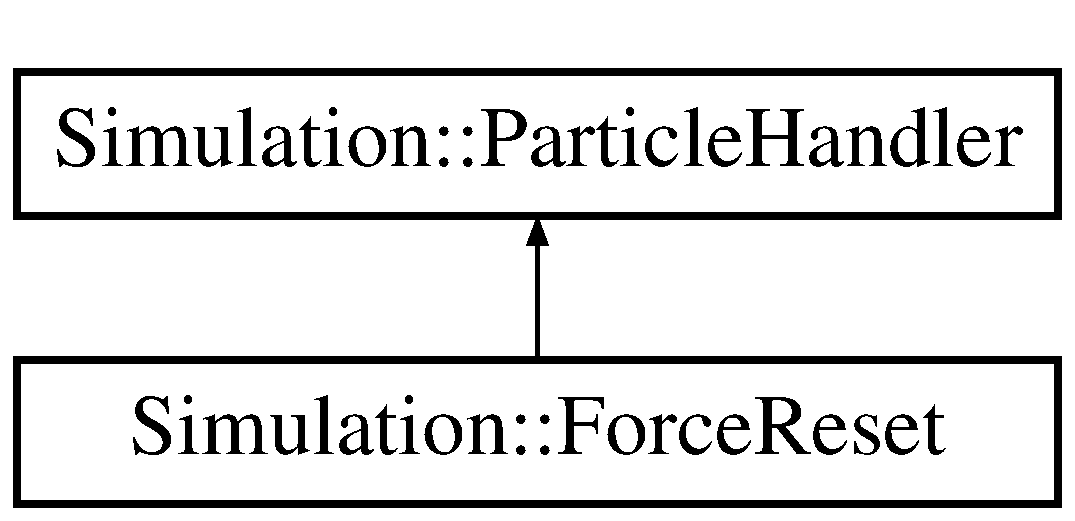
\includegraphics[height=2.000000cm]{classSimulation_1_1ForceReset}
\end{center}
\end{figure}
\subsection*{Public Member Functions}
\begin{DoxyCompactItemize}
\item 
void \hyperlink{classSimulation_1_1ForceReset_aae6e2c5b90fba7254e2213c02afdc5f1}{compute} (\hyperlink{classSimulation_1_1Particle}{Particle} \&p)
\begin{DoxyCompactList}\small\item\em Computes one single particle. \end{DoxyCompactList}\end{DoxyCompactItemize}


\subsection{Detailed Description}
resets force of zarticle to zero 

\subsection{Member Function Documentation}
\hypertarget{classSimulation_1_1ForceReset_aae6e2c5b90fba7254e2213c02afdc5f1}{\index{Simulation\-::\-Force\-Reset@{Simulation\-::\-Force\-Reset}!compute@{compute}}
\index{compute@{compute}!Simulation::ForceReset@{Simulation\-::\-Force\-Reset}}
\subsubsection[{compute}]{\setlength{\rightskip}{0pt plus 5cm}void Simulation\-::\-Force\-Reset\-::compute (
\begin{DoxyParamCaption}
\item[{{\bf Particle} \&}]{p}
\end{DoxyParamCaption}
)\hspace{0.3cm}{\ttfamily [inline]}, {\ttfamily [virtual]}}}\label{classSimulation_1_1ForceReset_aae6e2c5b90fba7254e2213c02afdc5f1}


Computes one single particle. 



Reimplemented from \hyperlink{classSimulation_1_1ParticleHandler_a6b1fc310603bc10093d50c674097fd25}{Simulation\-::\-Particle\-Handler}.



The documentation for this class was generated from the following file\-:\begin{DoxyCompactItemize}
\item 
src/\hyperlink{ParticleHandler_8h}{Particle\-Handler.\-h}\end{DoxyCompactItemize}

\hypertarget{classSimulation_1_1GravityHandler}{\section{Simulation\-:\-:Gravity\-Handler Class Reference}
\label{classSimulation_1_1GravityHandler}\index{Simulation\-::\-Gravity\-Handler@{Simulation\-::\-Gravity\-Handler}}
}


{\ttfamily \#include $<$Particle\-Handler.\-h$>$}

Inheritance diagram for Simulation\-:\-:Gravity\-Handler\-:\begin{figure}[H]
\begin{center}
\leavevmode
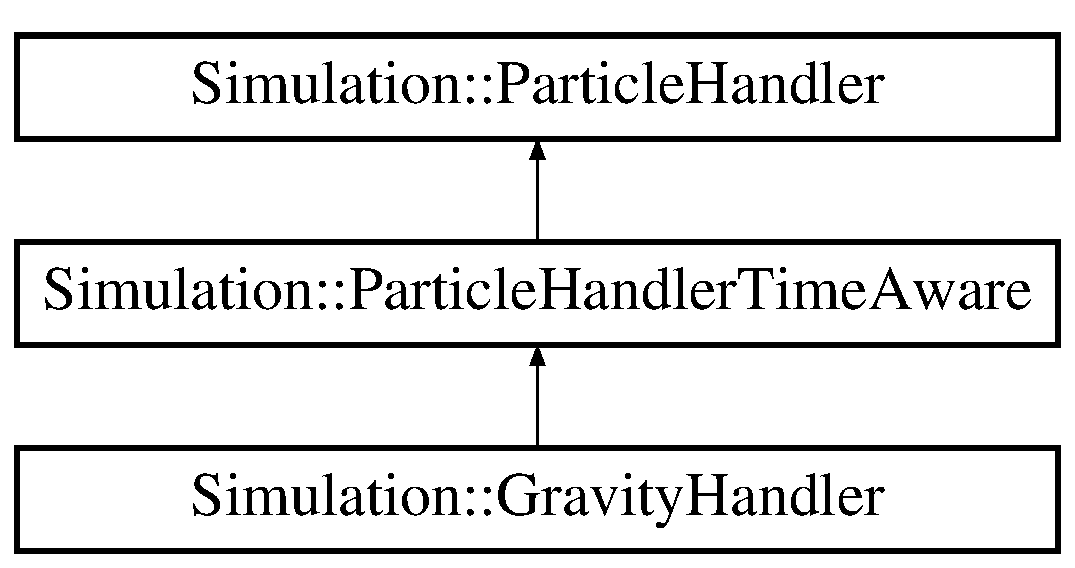
\includegraphics[height=3.000000cm]{classSimulation_1_1GravityHandler}
\end{center}
\end{figure}
\subsection*{Public Member Functions}
\begin{DoxyCompactItemize}
\item 
\hyperlink{classSimulation_1_1GravityHandler_abe61e3434323c7b7aaf52f00ac613bc9}{Gravity\-Handler} (double dt)
\item 
void \hyperlink{classSimulation_1_1GravityHandler_a7f5b0d36e4e8e3dd6eb54d364add0287}{compute} (\hyperlink{classSimulation_1_1Particle}{Particle} \&p)
\item 
void \hyperlink{classSimulation_1_1GravityHandler_a7805aa1b40a206d9fe3362a321d933ed}{compute} (\hyperlink{classSimulation_1_1Particle}{Particle} \&p1, \hyperlink{classSimulation_1_1Particle}{Particle} \&p2)
\item 
void \hyperlink{classSimulation_1_1GravityHandler_a4abb48d878ea825e6582ba0bf9ae5c0d}{compute\-Exclusive} (\hyperlink{classSimulation_1_1Particle}{Particle} \&p1, \hyperlink{classSimulation_1_1Particle}{Particle} \&p2)
\end{DoxyCompactItemize}
\subsection*{Additional Inherited Members}


\subsection{Constructor \& Destructor Documentation}
\hypertarget{classSimulation_1_1GravityHandler_abe61e3434323c7b7aaf52f00ac613bc9}{\index{Simulation\-::\-Gravity\-Handler@{Simulation\-::\-Gravity\-Handler}!Gravity\-Handler@{Gravity\-Handler}}
\index{Gravity\-Handler@{Gravity\-Handler}!Simulation::GravityHandler@{Simulation\-::\-Gravity\-Handler}}
\subsubsection[{Gravity\-Handler}]{\setlength{\rightskip}{0pt plus 5cm}Simulation\-::\-Gravity\-Handler\-::\-Gravity\-Handler (
\begin{DoxyParamCaption}
\item[{double}]{dt}
\end{DoxyParamCaption}
)\hspace{0.3cm}{\ttfamily [inline]}}}\label{classSimulation_1_1GravityHandler_abe61e3434323c7b7aaf52f00ac613bc9}


\subsection{Member Function Documentation}
\hypertarget{classSimulation_1_1GravityHandler_a7f5b0d36e4e8e3dd6eb54d364add0287}{\index{Simulation\-::\-Gravity\-Handler@{Simulation\-::\-Gravity\-Handler}!compute@{compute}}
\index{compute@{compute}!Simulation::GravityHandler@{Simulation\-::\-Gravity\-Handler}}
\subsubsection[{compute}]{\setlength{\rightskip}{0pt plus 5cm}void Simulation\-::\-Gravity\-Handler\-::compute (
\begin{DoxyParamCaption}
\item[{{\bf Particle} \&}]{p}
\end{DoxyParamCaption}
)\hspace{0.3cm}{\ttfamily [inline]}, {\ttfamily [virtual]}}}\label{classSimulation_1_1GravityHandler_a7f5b0d36e4e8e3dd6eb54d364add0287}


Reimplemented from \hyperlink{classSimulation_1_1ParticleHandler_a6b1fc310603bc10093d50c674097fd25}{Simulation\-::\-Particle\-Handler}.

\hypertarget{classSimulation_1_1GravityHandler_a7805aa1b40a206d9fe3362a321d933ed}{\index{Simulation\-::\-Gravity\-Handler@{Simulation\-::\-Gravity\-Handler}!compute@{compute}}
\index{compute@{compute}!Simulation::GravityHandler@{Simulation\-::\-Gravity\-Handler}}
\subsubsection[{compute}]{\setlength{\rightskip}{0pt plus 5cm}void Simulation\-::\-Gravity\-Handler\-::compute (
\begin{DoxyParamCaption}
\item[{{\bf Particle} \&}]{p1, }
\item[{{\bf Particle} \&}]{p2}
\end{DoxyParamCaption}
)\hspace{0.3cm}{\ttfamily [inline]}, {\ttfamily [virtual]}}}\label{classSimulation_1_1GravityHandler_a7805aa1b40a206d9fe3362a321d933ed}


Reimplemented from \hyperlink{classSimulation_1_1ParticleHandler_a013ad557c6892ed2287db090192144ea}{Simulation\-::\-Particle\-Handler}.

\hypertarget{classSimulation_1_1GravityHandler_a4abb48d878ea825e6582ba0bf9ae5c0d}{\index{Simulation\-::\-Gravity\-Handler@{Simulation\-::\-Gravity\-Handler}!compute\-Exclusive@{compute\-Exclusive}}
\index{compute\-Exclusive@{compute\-Exclusive}!Simulation::GravityHandler@{Simulation\-::\-Gravity\-Handler}}
\subsubsection[{compute\-Exclusive}]{\setlength{\rightskip}{0pt plus 5cm}void Simulation\-::\-Gravity\-Handler\-::compute\-Exclusive (
\begin{DoxyParamCaption}
\item[{{\bf Particle} \&}]{p1, }
\item[{{\bf Particle} \&}]{p2}
\end{DoxyParamCaption}
)\hspace{0.3cm}{\ttfamily [inline]}, {\ttfamily [virtual]}}}\label{classSimulation_1_1GravityHandler_a4abb48d878ea825e6582ba0bf9ae5c0d}


Reimplemented from \hyperlink{classSimulation_1_1ParticleHandler_a4a1caeb40ada4f410fec9244bda4af69}{Simulation\-::\-Particle\-Handler}.



The documentation for this class was generated from the following file\-:\begin{DoxyCompactItemize}
\item 
src/\hyperlink{ParticleHandler_8h}{Particle\-Handler.\-h}\end{DoxyCompactItemize}

\hypertarget{classSimulation_1_1LennardJonesHandler}{\section{Simulation\-:\-:Lennard\-Jones\-Handler Class Reference}
\label{classSimulation_1_1LennardJonesHandler}\index{Simulation\-::\-Lennard\-Jones\-Handler@{Simulation\-::\-Lennard\-Jones\-Handler}}
}


{\ttfamily \#include $<$Particle\-Handler.\-h$>$}

Inheritance diagram for Simulation\-:\-:Lennard\-Jones\-Handler\-:\begin{figure}[H]
\begin{center}
\leavevmode
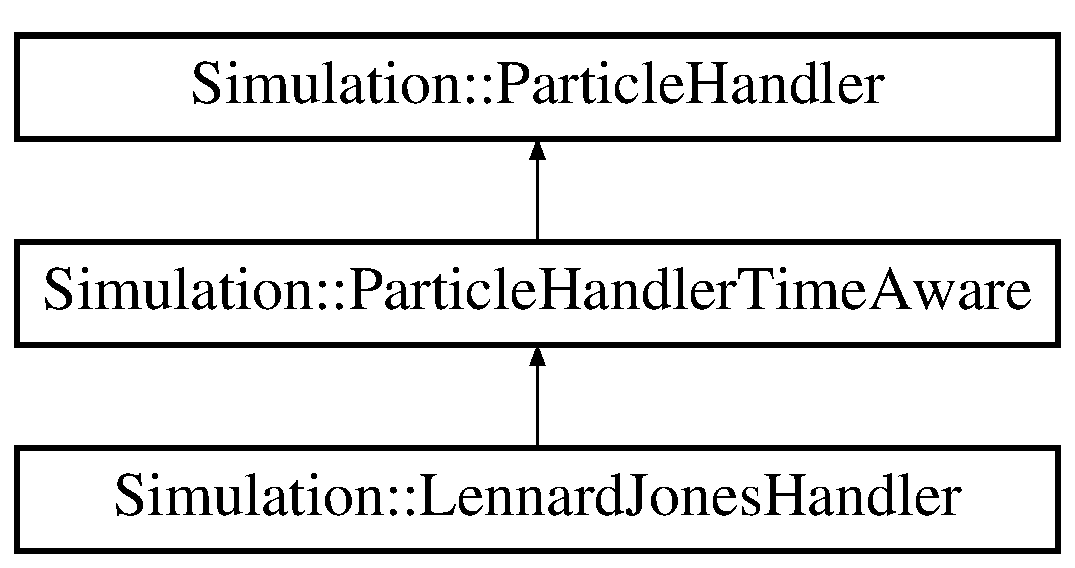
\includegraphics[height=3.000000cm]{classSimulation_1_1LennardJonesHandler}
\end{center}
\end{figure}
\subsection*{Public Member Functions}
\begin{DoxyCompactItemize}
\item 
\hyperlink{classSimulation_1_1LennardJonesHandler_a1eea638f715656e842824a9f9fa56a01}{Lennard\-Jones\-Handler} (double dt)
\item 
void \hyperlink{classSimulation_1_1LennardJonesHandler_aa2a7d4ce850ece69663918a7cfc4072f}{compute} (\hyperlink{classSimulation_1_1Particle}{Particle} \&p)
\item 
void \hyperlink{classSimulation_1_1LennardJonesHandler_a81842168e68a61cb75448f91bc27f99c}{compute} (\hyperlink{classSimulation_1_1Particle}{Particle} \&p1, \hyperlink{classSimulation_1_1Particle}{Particle} \&p2)
\item 
void \hyperlink{classSimulation_1_1LennardJonesHandler_ac16127a588f6e8598dc2598d1224517f}{compute\-Exclusive} (\hyperlink{classSimulation_1_1Particle}{Particle} \&p1, \hyperlink{classSimulation_1_1Particle}{Particle} \&p2)
\end{DoxyCompactItemize}
\subsection*{Additional Inherited Members}


\subsection{Constructor \& Destructor Documentation}
\hypertarget{classSimulation_1_1LennardJonesHandler_a1eea638f715656e842824a9f9fa56a01}{\index{Simulation\-::\-Lennard\-Jones\-Handler@{Simulation\-::\-Lennard\-Jones\-Handler}!Lennard\-Jones\-Handler@{Lennard\-Jones\-Handler}}
\index{Lennard\-Jones\-Handler@{Lennard\-Jones\-Handler}!Simulation::LennardJonesHandler@{Simulation\-::\-Lennard\-Jones\-Handler}}
\subsubsection[{Lennard\-Jones\-Handler}]{\setlength{\rightskip}{0pt plus 5cm}Simulation\-::\-Lennard\-Jones\-Handler\-::\-Lennard\-Jones\-Handler (
\begin{DoxyParamCaption}
\item[{double}]{dt}
\end{DoxyParamCaption}
)\hspace{0.3cm}{\ttfamily [inline]}}}\label{classSimulation_1_1LennardJonesHandler_a1eea638f715656e842824a9f9fa56a01}


\subsection{Member Function Documentation}
\hypertarget{classSimulation_1_1LennardJonesHandler_aa2a7d4ce850ece69663918a7cfc4072f}{\index{Simulation\-::\-Lennard\-Jones\-Handler@{Simulation\-::\-Lennard\-Jones\-Handler}!compute@{compute}}
\index{compute@{compute}!Simulation::LennardJonesHandler@{Simulation\-::\-Lennard\-Jones\-Handler}}
\subsubsection[{compute}]{\setlength{\rightskip}{0pt plus 5cm}void Simulation\-::\-Lennard\-Jones\-Handler\-::compute (
\begin{DoxyParamCaption}
\item[{{\bf Particle} \&}]{p}
\end{DoxyParamCaption}
)\hspace{0.3cm}{\ttfamily [inline]}, {\ttfamily [virtual]}}}\label{classSimulation_1_1LennardJonesHandler_aa2a7d4ce850ece69663918a7cfc4072f}


Reimplemented from \hyperlink{classSimulation_1_1ParticleHandler_a6b1fc310603bc10093d50c674097fd25}{Simulation\-::\-Particle\-Handler}.

\hypertarget{classSimulation_1_1LennardJonesHandler_a81842168e68a61cb75448f91bc27f99c}{\index{Simulation\-::\-Lennard\-Jones\-Handler@{Simulation\-::\-Lennard\-Jones\-Handler}!compute@{compute}}
\index{compute@{compute}!Simulation::LennardJonesHandler@{Simulation\-::\-Lennard\-Jones\-Handler}}
\subsubsection[{compute}]{\setlength{\rightskip}{0pt plus 5cm}void Simulation\-::\-Lennard\-Jones\-Handler\-::compute (
\begin{DoxyParamCaption}
\item[{{\bf Particle} \&}]{p1, }
\item[{{\bf Particle} \&}]{p2}
\end{DoxyParamCaption}
)\hspace{0.3cm}{\ttfamily [inline]}, {\ttfamily [virtual]}}}\label{classSimulation_1_1LennardJonesHandler_a81842168e68a61cb75448f91bc27f99c}


Reimplemented from \hyperlink{classSimulation_1_1ParticleHandler_a013ad557c6892ed2287db090192144ea}{Simulation\-::\-Particle\-Handler}.

\hypertarget{classSimulation_1_1LennardJonesHandler_ac16127a588f6e8598dc2598d1224517f}{\index{Simulation\-::\-Lennard\-Jones\-Handler@{Simulation\-::\-Lennard\-Jones\-Handler}!compute\-Exclusive@{compute\-Exclusive}}
\index{compute\-Exclusive@{compute\-Exclusive}!Simulation::LennardJonesHandler@{Simulation\-::\-Lennard\-Jones\-Handler}}
\subsubsection[{compute\-Exclusive}]{\setlength{\rightskip}{0pt plus 5cm}void Simulation\-::\-Lennard\-Jones\-Handler\-::compute\-Exclusive (
\begin{DoxyParamCaption}
\item[{{\bf Particle} \&}]{p1, }
\item[{{\bf Particle} \&}]{p2}
\end{DoxyParamCaption}
)\hspace{0.3cm}{\ttfamily [inline]}, {\ttfamily [virtual]}}}\label{classSimulation_1_1LennardJonesHandler_ac16127a588f6e8598dc2598d1224517f}


Reimplemented from \hyperlink{classSimulation_1_1ParticleHandler_a4a1caeb40ada4f410fec9244bda4af69}{Simulation\-::\-Particle\-Handler}.



The documentation for this class was generated from the following file\-:\begin{DoxyCompactItemize}
\item 
src/\hyperlink{ParticleHandler_8h}{Particle\-Handler.\-h}\end{DoxyCompactItemize}

\hypertarget{classSimulation_1_1Particle}{\section{Simulation\-:\-:Particle Class Reference}
\label{classSimulation_1_1Particle}\index{Simulation\-::\-Particle@{Simulation\-::\-Particle}}
}


Definition for particle that participates in \hyperlink{namespaceSimulation}{Simulation}.  




{\ttfamily \#include $<$Particle.\-h$>$}

\subsection*{Public Member Functions}
\begin{DoxyCompactItemize}
\item 
\hyperlink{classSimulation_1_1Particle_ac41912df0ce136018e70f568aef0d6dd}{Particle} (int \hyperlink{classtype}{type}, bool vivible=true)
\item 
\hyperlink{classSimulation_1_1Particle_a24b04cb7c6f7ea4242d25c410f44ae56}{Particle} (const \hyperlink{classSimulation_1_1Particle}{Particle} \&other)
\item 
\hyperlink{classSimulation_1_1Particle_adb4ed8bc5618347a28cbbdaf0047309c}{Particle} (\hyperlink{classutils_1_1Vector}{utils\-::\-Vector}$<$ double, 3 $>$ x\-\_\-arg, \hyperlink{classutils_1_1Vector}{utils\-::\-Vector}$<$ double, 3 $>$ v\-\_\-arg, int \hyperlink{classtype}{type}, bool vis=true)
\item 
virtual \hyperlink{classSimulation_1_1Particle_ad030d0fe7b88cf81744b127c99244ff4}{$\sim$\-Particle} ()
\item 
\hyperlink{classutils_1_1Vector}{utils\-::\-Vector}$<$ double, 3 $>$ \& \hyperlink{classSimulation_1_1Particle_ab7ade5dc156dfa0234aa0323564e46ed}{get\-X} ()
\item 
\hyperlink{classutils_1_1Vector}{utils\-::\-Vector}$<$ double, 3 $>$ \& \hyperlink{classSimulation_1_1Particle_acd84c445e2bd5f5280a00e76cfe73fe0}{get\-F} ()
\item 
\hyperlink{classutils_1_1Vector}{utils\-::\-Vector}$<$ double, 3 $>$ \& \hyperlink{classSimulation_1_1Particle_a1204435fc08c697b0fea230616d1bbdf}{get\-Old\-F} ()
\item 
\hyperlink{classutils_1_1Vector}{utils\-::\-Vector}$<$ double, 3 $>$ \& \hyperlink{classSimulation_1_1Particle_aaf3ecbc6e1e31b259fe239461ba13dbd}{get\-V} ()
\item 
double \hyperlink{classSimulation_1_1Particle_aa1ca800f9be9dd4bd6c604f608095b24}{get\-M} ()
\item 
double \hyperlink{classSimulation_1_1Particle_ad449ae6dec0265efb91b7a714563fa12}{get\-E} ()
\item 
double \hyperlink{classSimulation_1_1Particle_abef7a42b32e938861884c958019cf41b}{get\-O} ()
\item 
int \hyperlink{classSimulation_1_1Particle_a0581d7b629eb17ac5bef8e934852ca8b}{get\-Type} ()
\item 
void \hyperlink{classSimulation_1_1Particle_a03487469e558306b9d770fb547ab23a3}{set\-Type} (int t)
\item 
int \hyperlink{classSimulation_1_1Particle_a7e74baf0c324e1474f6e5a4a072e5e8b}{get\-Cell} ()
\item 
void \hyperlink{classSimulation_1_1Particle_a701c977a46c66ac52c901eb9ee517389}{set\-Cell} (int c)
\item 
bool \hyperlink{classSimulation_1_1Particle_a28a301c6d1f08f5b77bd091d79872517}{is\-Visible} ()
\item 
bool \hyperlink{classSimulation_1_1Particle_a5034babb77618a56e00927d8891afabe}{operator==} (\hyperlink{classSimulation_1_1Particle}{Particle} \&other)
\item 
std\-::string \hyperlink{classSimulation_1_1Particle_a07d071a0f91f8ce7413201a6db3afe7b}{to\-String} ()
\end{DoxyCompactItemize}
\subsection*{Private Attributes}
\begin{DoxyCompactItemize}
\item 
\hyperlink{classutils_1_1Vector}{utils\-::\-Vector}$<$ double, 3 $>$ \hyperlink{classSimulation_1_1Particle_a37114cf327ef0591939f157489434bde}{x}
\begin{DoxyCompactList}\small\item\em The position of the particle. \end{DoxyCompactList}\item 
\hyperlink{classutils_1_1Vector}{utils\-::\-Vector}$<$ double, 3 $>$ \hyperlink{classSimulation_1_1Particle_aedd9ec08978292732fc38dd6d93dc3b4}{v}
\begin{DoxyCompactList}\small\item\em The velocity of the particle. \end{DoxyCompactList}\item 
\hyperlink{classutils_1_1Vector}{utils\-::\-Vector}$<$ double, 3 $>$ \hyperlink{classSimulation_1_1Particle_a54c7b7f1cb33876abdbd505d06c9b499}{f}
\begin{DoxyCompactList}\small\item\em The force effective on this particle. \end{DoxyCompactList}\item 
\hyperlink{classutils_1_1Vector}{utils\-::\-Vector}$<$ double, 3 $>$ \hyperlink{classSimulation_1_1Particle_a80cc4684069bff79cb7d91c25237141f}{old\-\_\-f}
\begin{DoxyCompactList}\small\item\em The force wich was effective on this particle. \end{DoxyCompactList}\item 
int \hyperlink{classSimulation_1_1Particle_aeb6388e2a21c03c7e1582eb4eeb5efb3}{type}
\begin{DoxyCompactList}\small\item\em Type, defines properties of particle. \end{DoxyCompactList}\item 
int \hyperlink{classSimulation_1_1Particle_aebbb649086b757029a513e09adf76d4b}{cell}
\begin{DoxyCompactList}\small\item\em Cell which holds particle. \end{DoxyCompactList}\item 
bool \hyperlink{classSimulation_1_1Particle_a20e56ab0bd4071b5cb479775742f2cfe}{visible}
\end{DoxyCompactItemize}


\subsection{Detailed Description}
Definition for particle that participates in \hyperlink{namespaceSimulation}{Simulation}. 

\subsection{Constructor \& Destructor Documentation}
\hypertarget{classSimulation_1_1Particle_ac41912df0ce136018e70f568aef0d6dd}{\index{Simulation\-::\-Particle@{Simulation\-::\-Particle}!Particle@{Particle}}
\index{Particle@{Particle}!Simulation::Particle@{Simulation\-::\-Particle}}
\subsubsection[{Particle}]{\setlength{\rightskip}{0pt plus 5cm}Particle\-::\-Particle (
\begin{DoxyParamCaption}
\item[{int}]{type, }
\item[{bool}]{vivible = {\ttfamily true}}
\end{DoxyParamCaption}
)}}\label{classSimulation_1_1Particle_ac41912df0ce136018e70f568aef0d6dd}
\hypertarget{classSimulation_1_1Particle_a24b04cb7c6f7ea4242d25c410f44ae56}{\index{Simulation\-::\-Particle@{Simulation\-::\-Particle}!Particle@{Particle}}
\index{Particle@{Particle}!Simulation::Particle@{Simulation\-::\-Particle}}
\subsubsection[{Particle}]{\setlength{\rightskip}{0pt plus 5cm}Particle\-::\-Particle (
\begin{DoxyParamCaption}
\item[{const {\bf Particle} \&}]{other}
\end{DoxyParamCaption}
)}}\label{classSimulation_1_1Particle_a24b04cb7c6f7ea4242d25c410f44ae56}
\hypertarget{classSimulation_1_1Particle_adb4ed8bc5618347a28cbbdaf0047309c}{\index{Simulation\-::\-Particle@{Simulation\-::\-Particle}!Particle@{Particle}}
\index{Particle@{Particle}!Simulation::Particle@{Simulation\-::\-Particle}}
\subsubsection[{Particle}]{\setlength{\rightskip}{0pt plus 5cm}Particle\-::\-Particle (
\begin{DoxyParamCaption}
\item[{{\bf utils\-::\-Vector}$<$ double, 3 $>$}]{x\-\_\-arg, }
\item[{{\bf utils\-::\-Vector}$<$ double, 3 $>$}]{v\-\_\-arg, }
\item[{int}]{type, }
\item[{bool}]{vis = {\ttfamily true}}
\end{DoxyParamCaption}
)}}\label{classSimulation_1_1Particle_adb4ed8bc5618347a28cbbdaf0047309c}
\hypertarget{classSimulation_1_1Particle_ad030d0fe7b88cf81744b127c99244ff4}{\index{Simulation\-::\-Particle@{Simulation\-::\-Particle}!$\sim$\-Particle@{$\sim$\-Particle}}
\index{$\sim$\-Particle@{$\sim$\-Particle}!Simulation::Particle@{Simulation\-::\-Particle}}
\subsubsection[{$\sim$\-Particle}]{\setlength{\rightskip}{0pt plus 5cm}Particle\-::$\sim$\-Particle (
\begin{DoxyParamCaption}
{}
\end{DoxyParamCaption}
)\hspace{0.3cm}{\ttfamily [virtual]}}}\label{classSimulation_1_1Particle_ad030d0fe7b88cf81744b127c99244ff4}


\subsection{Member Function Documentation}
\hypertarget{classSimulation_1_1Particle_a7e74baf0c324e1474f6e5a4a072e5e8b}{\index{Simulation\-::\-Particle@{Simulation\-::\-Particle}!get\-Cell@{get\-Cell}}
\index{get\-Cell@{get\-Cell}!Simulation::Particle@{Simulation\-::\-Particle}}
\subsubsection[{get\-Cell}]{\setlength{\rightskip}{0pt plus 5cm}int Particle\-::get\-Cell (
\begin{DoxyParamCaption}
{}
\end{DoxyParamCaption}
)}}\label{classSimulation_1_1Particle_a7e74baf0c324e1474f6e5a4a072e5e8b}
\hypertarget{classSimulation_1_1Particle_ad449ae6dec0265efb91b7a714563fa12}{\index{Simulation\-::\-Particle@{Simulation\-::\-Particle}!get\-E@{get\-E}}
\index{get\-E@{get\-E}!Simulation::Particle@{Simulation\-::\-Particle}}
\subsubsection[{get\-E}]{\setlength{\rightskip}{0pt plus 5cm}double Particle\-::get\-E (
\begin{DoxyParamCaption}
{}
\end{DoxyParamCaption}
)}}\label{classSimulation_1_1Particle_ad449ae6dec0265efb91b7a714563fa12}
\hypertarget{classSimulation_1_1Particle_acd84c445e2bd5f5280a00e76cfe73fe0}{\index{Simulation\-::\-Particle@{Simulation\-::\-Particle}!get\-F@{get\-F}}
\index{get\-F@{get\-F}!Simulation::Particle@{Simulation\-::\-Particle}}
\subsubsection[{get\-F}]{\setlength{\rightskip}{0pt plus 5cm}{\bf utils\-::\-Vector}$<$ double, 3 $>$ \& Particle\-::get\-F (
\begin{DoxyParamCaption}
{}
\end{DoxyParamCaption}
)}}\label{classSimulation_1_1Particle_acd84c445e2bd5f5280a00e76cfe73fe0}
\hypertarget{classSimulation_1_1Particle_aa1ca800f9be9dd4bd6c604f608095b24}{\index{Simulation\-::\-Particle@{Simulation\-::\-Particle}!get\-M@{get\-M}}
\index{get\-M@{get\-M}!Simulation::Particle@{Simulation\-::\-Particle}}
\subsubsection[{get\-M}]{\setlength{\rightskip}{0pt plus 5cm}double Particle\-::get\-M (
\begin{DoxyParamCaption}
{}
\end{DoxyParamCaption}
)}}\label{classSimulation_1_1Particle_aa1ca800f9be9dd4bd6c604f608095b24}
\hypertarget{classSimulation_1_1Particle_abef7a42b32e938861884c958019cf41b}{\index{Simulation\-::\-Particle@{Simulation\-::\-Particle}!get\-O@{get\-O}}
\index{get\-O@{get\-O}!Simulation::Particle@{Simulation\-::\-Particle}}
\subsubsection[{get\-O}]{\setlength{\rightskip}{0pt plus 5cm}double Particle\-::get\-O (
\begin{DoxyParamCaption}
{}
\end{DoxyParamCaption}
)}}\label{classSimulation_1_1Particle_abef7a42b32e938861884c958019cf41b}
\hypertarget{classSimulation_1_1Particle_a1204435fc08c697b0fea230616d1bbdf}{\index{Simulation\-::\-Particle@{Simulation\-::\-Particle}!get\-Old\-F@{get\-Old\-F}}
\index{get\-Old\-F@{get\-Old\-F}!Simulation::Particle@{Simulation\-::\-Particle}}
\subsubsection[{get\-Old\-F}]{\setlength{\rightskip}{0pt plus 5cm}{\bf utils\-::\-Vector}$<$ double, 3 $>$ \& Particle\-::get\-Old\-F (
\begin{DoxyParamCaption}
{}
\end{DoxyParamCaption}
)}}\label{classSimulation_1_1Particle_a1204435fc08c697b0fea230616d1bbdf}
\hypertarget{classSimulation_1_1Particle_a0581d7b629eb17ac5bef8e934852ca8b}{\index{Simulation\-::\-Particle@{Simulation\-::\-Particle}!get\-Type@{get\-Type}}
\index{get\-Type@{get\-Type}!Simulation::Particle@{Simulation\-::\-Particle}}
\subsubsection[{get\-Type}]{\setlength{\rightskip}{0pt plus 5cm}int Particle\-::get\-Type (
\begin{DoxyParamCaption}
{}
\end{DoxyParamCaption}
)}}\label{classSimulation_1_1Particle_a0581d7b629eb17ac5bef8e934852ca8b}
\hypertarget{classSimulation_1_1Particle_aaf3ecbc6e1e31b259fe239461ba13dbd}{\index{Simulation\-::\-Particle@{Simulation\-::\-Particle}!get\-V@{get\-V}}
\index{get\-V@{get\-V}!Simulation::Particle@{Simulation\-::\-Particle}}
\subsubsection[{get\-V}]{\setlength{\rightskip}{0pt plus 5cm}{\bf utils\-::\-Vector}$<$ double, 3 $>$ \& Particle\-::get\-V (
\begin{DoxyParamCaption}
{}
\end{DoxyParamCaption}
)}}\label{classSimulation_1_1Particle_aaf3ecbc6e1e31b259fe239461ba13dbd}
\hypertarget{classSimulation_1_1Particle_ab7ade5dc156dfa0234aa0323564e46ed}{\index{Simulation\-::\-Particle@{Simulation\-::\-Particle}!get\-X@{get\-X}}
\index{get\-X@{get\-X}!Simulation::Particle@{Simulation\-::\-Particle}}
\subsubsection[{get\-X}]{\setlength{\rightskip}{0pt plus 5cm}{\bf utils\-::\-Vector}$<$ double, 3 $>$ \& Particle\-::get\-X (
\begin{DoxyParamCaption}
{}
\end{DoxyParamCaption}
)}}\label{classSimulation_1_1Particle_ab7ade5dc156dfa0234aa0323564e46ed}
\hypertarget{classSimulation_1_1Particle_a28a301c6d1f08f5b77bd091d79872517}{\index{Simulation\-::\-Particle@{Simulation\-::\-Particle}!is\-Visible@{is\-Visible}}
\index{is\-Visible@{is\-Visible}!Simulation::Particle@{Simulation\-::\-Particle}}
\subsubsection[{is\-Visible}]{\setlength{\rightskip}{0pt plus 5cm}bool Particle\-::is\-Visible (
\begin{DoxyParamCaption}
{}
\end{DoxyParamCaption}
)}}\label{classSimulation_1_1Particle_a28a301c6d1f08f5b77bd091d79872517}
\hypertarget{classSimulation_1_1Particle_a5034babb77618a56e00927d8891afabe}{\index{Simulation\-::\-Particle@{Simulation\-::\-Particle}!operator==@{operator==}}
\index{operator==@{operator==}!Simulation::Particle@{Simulation\-::\-Particle}}
\subsubsection[{operator==}]{\setlength{\rightskip}{0pt plus 5cm}bool Particle\-::operator== (
\begin{DoxyParamCaption}
\item[{{\bf Particle} \&}]{other}
\end{DoxyParamCaption}
)}}\label{classSimulation_1_1Particle_a5034babb77618a56e00927d8891afabe}
\hypertarget{classSimulation_1_1Particle_a701c977a46c66ac52c901eb9ee517389}{\index{Simulation\-::\-Particle@{Simulation\-::\-Particle}!set\-Cell@{set\-Cell}}
\index{set\-Cell@{set\-Cell}!Simulation::Particle@{Simulation\-::\-Particle}}
\subsubsection[{set\-Cell}]{\setlength{\rightskip}{0pt plus 5cm}void Particle\-::set\-Cell (
\begin{DoxyParamCaption}
\item[{int}]{c}
\end{DoxyParamCaption}
)}}\label{classSimulation_1_1Particle_a701c977a46c66ac52c901eb9ee517389}
\hypertarget{classSimulation_1_1Particle_a03487469e558306b9d770fb547ab23a3}{\index{Simulation\-::\-Particle@{Simulation\-::\-Particle}!set\-Type@{set\-Type}}
\index{set\-Type@{set\-Type}!Simulation::Particle@{Simulation\-::\-Particle}}
\subsubsection[{set\-Type}]{\setlength{\rightskip}{0pt plus 5cm}void Particle\-::set\-Type (
\begin{DoxyParamCaption}
\item[{int}]{t}
\end{DoxyParamCaption}
)}}\label{classSimulation_1_1Particle_a03487469e558306b9d770fb547ab23a3}
\hypertarget{classSimulation_1_1Particle_a07d071a0f91f8ce7413201a6db3afe7b}{\index{Simulation\-::\-Particle@{Simulation\-::\-Particle}!to\-String@{to\-String}}
\index{to\-String@{to\-String}!Simulation::Particle@{Simulation\-::\-Particle}}
\subsubsection[{to\-String}]{\setlength{\rightskip}{0pt plus 5cm}std\-::string Particle\-::to\-String (
\begin{DoxyParamCaption}
{}
\end{DoxyParamCaption}
)}}\label{classSimulation_1_1Particle_a07d071a0f91f8ce7413201a6db3afe7b}


\subsection{Member Data Documentation}
\hypertarget{classSimulation_1_1Particle_aebbb649086b757029a513e09adf76d4b}{\index{Simulation\-::\-Particle@{Simulation\-::\-Particle}!cell@{cell}}
\index{cell@{cell}!Simulation::Particle@{Simulation\-::\-Particle}}
\subsubsection[{cell}]{\setlength{\rightskip}{0pt plus 5cm}int Simulation\-::\-Particle\-::cell\hspace{0.3cm}{\ttfamily [private]}}}\label{classSimulation_1_1Particle_aebbb649086b757029a513e09adf76d4b}


Cell which holds particle. 

\hypertarget{classSimulation_1_1Particle_a54c7b7f1cb33876abdbd505d06c9b499}{\index{Simulation\-::\-Particle@{Simulation\-::\-Particle}!f@{f}}
\index{f@{f}!Simulation::Particle@{Simulation\-::\-Particle}}
\subsubsection[{f}]{\setlength{\rightskip}{0pt plus 5cm}{\bf utils\-::\-Vector}$<$double, 3$>$ Simulation\-::\-Particle\-::f\hspace{0.3cm}{\ttfamily [private]}}}\label{classSimulation_1_1Particle_a54c7b7f1cb33876abdbd505d06c9b499}


The force effective on this particle. 

\hypertarget{classSimulation_1_1Particle_a80cc4684069bff79cb7d91c25237141f}{\index{Simulation\-::\-Particle@{Simulation\-::\-Particle}!old\-\_\-f@{old\-\_\-f}}
\index{old\-\_\-f@{old\-\_\-f}!Simulation::Particle@{Simulation\-::\-Particle}}
\subsubsection[{old\-\_\-f}]{\setlength{\rightskip}{0pt plus 5cm}{\bf utils\-::\-Vector}$<$double, 3$>$ Simulation\-::\-Particle\-::old\-\_\-f\hspace{0.3cm}{\ttfamily [private]}}}\label{classSimulation_1_1Particle_a80cc4684069bff79cb7d91c25237141f}


The force wich was effective on this particle. 

\hypertarget{classSimulation_1_1Particle_aeb6388e2a21c03c7e1582eb4eeb5efb3}{\index{Simulation\-::\-Particle@{Simulation\-::\-Particle}!type@{type}}
\index{type@{type}!Simulation::Particle@{Simulation\-::\-Particle}}
\subsubsection[{type}]{\setlength{\rightskip}{0pt plus 5cm}int Simulation\-::\-Particle\-::type\hspace{0.3cm}{\ttfamily [private]}}}\label{classSimulation_1_1Particle_aeb6388e2a21c03c7e1582eb4eeb5efb3}


Type, defines properties of particle. 

\hypertarget{classSimulation_1_1Particle_aedd9ec08978292732fc38dd6d93dc3b4}{\index{Simulation\-::\-Particle@{Simulation\-::\-Particle}!v@{v}}
\index{v@{v}!Simulation::Particle@{Simulation\-::\-Particle}}
\subsubsection[{v}]{\setlength{\rightskip}{0pt plus 5cm}{\bf utils\-::\-Vector}$<$double, 3$>$ Simulation\-::\-Particle\-::v\hspace{0.3cm}{\ttfamily [private]}}}\label{classSimulation_1_1Particle_aedd9ec08978292732fc38dd6d93dc3b4}


The velocity of the particle. 

\hypertarget{classSimulation_1_1Particle_a20e56ab0bd4071b5cb479775742f2cfe}{\index{Simulation\-::\-Particle@{Simulation\-::\-Particle}!visible@{visible}}
\index{visible@{visible}!Simulation::Particle@{Simulation\-::\-Particle}}
\subsubsection[{visible}]{\setlength{\rightskip}{0pt plus 5cm}bool Simulation\-::\-Particle\-::visible\hspace{0.3cm}{\ttfamily [private]}}}\label{classSimulation_1_1Particle_a20e56ab0bd4071b5cb479775742f2cfe}
\hypertarget{classSimulation_1_1Particle_a37114cf327ef0591939f157489434bde}{\index{Simulation\-::\-Particle@{Simulation\-::\-Particle}!x@{x}}
\index{x@{x}!Simulation::Particle@{Simulation\-::\-Particle}}
\subsubsection[{x}]{\setlength{\rightskip}{0pt plus 5cm}{\bf utils\-::\-Vector}$<$double, 3$>$ Simulation\-::\-Particle\-::x\hspace{0.3cm}{\ttfamily [private]}}}\label{classSimulation_1_1Particle_a37114cf327ef0591939f157489434bde}


The position of the particle. 



The documentation for this class was generated from the following files\-:\begin{DoxyCompactItemize}
\item 
src/\hyperlink{Particle_8h}{Particle.\-h}\item 
src/\hyperlink{Particle_8cpp}{Particle.\-cpp}\end{DoxyCompactItemize}

\hypertarget{classSimulation_1_1ParticleCell}{\section{Simulation\-:\-:Particle\-Cell Class Reference}
\label{classSimulation_1_1ParticleCell}\index{Simulation\-::\-Particle\-Cell@{Simulation\-::\-Particle\-Cell}}
}


Stores pointers to particles which lie in this cell.  




{\ttfamily \#include $<$Particle\-Container.\-h$>$}

\subsection*{Public Types}
\begin{DoxyCompactItemize}
\item 
enum \hyperlink{classSimulation_1_1ParticleCell_a2212779392dcf6befecc55da1ec5356c}{Cell\-Type} \{ \\*
\hyperlink{classSimulation_1_1ParticleCell_a2212779392dcf6befecc55da1ec5356caa37d40bf1097ce2043342c9a4d52182b}{Inner\-Cell}, 
\hyperlink{classSimulation_1_1ParticleCell_a2212779392dcf6befecc55da1ec5356ca9b7b3132a0d07ce3c1ec88e586bf2eb0}{Left\-Boundary}, 
\hyperlink{classSimulation_1_1ParticleCell_a2212779392dcf6befecc55da1ec5356ca424b56d6cea2bc492efd833bd3b07cdb}{Right\-Boundary}, 
\hyperlink{classSimulation_1_1ParticleCell_a2212779392dcf6befecc55da1ec5356ca10c2e4dddb9ca58b6b4526d5996ad288}{Bottom\-Boundary}, 
\\*
\hyperlink{classSimulation_1_1ParticleCell_a2212779392dcf6befecc55da1ec5356ca10d23b8bf6686ae323d3af3dcb61c368}{Top\-Boundary}, 
\hyperlink{classSimulation_1_1ParticleCell_a2212779392dcf6befecc55da1ec5356cac0b8b9d11a7514e08bf149a2246ceb7f}{Corner}
 \}
\end{DoxyCompactItemize}
\subsection*{Public Member Functions}
\begin{DoxyCompactItemize}
\item 
\hyperlink{classSimulation_1_1ParticleCell_a2a61d645388b8c75d17d3d7c63640674}{Particle\-Cell} (int i, \hyperlink{classutils_1_1Vector}{utils\-::\-Vector}$<$ double, 3 $>$ \&\hyperlink{classSimulation_1_1ParticleCell_a4bb88bb8f5196cf9ad558f304fe33404}{pos}, double $\ast$r)
\item 
\hyperlink{classSimulation_1_1ParticleCell_a2212779392dcf6befecc55da1ec5356c}{Cell\-Type} \& \hyperlink{classSimulation_1_1ParticleCell_a17d535f80c15a7abcab53d5230bbc524}{cell\-Type} ()
\item 
void \hyperlink{classSimulation_1_1ParticleCell_a780c301fa5e209ac14e36cc642e6450b}{insert} (\hyperlink{classSimulation_1_1Particle}{Particle} $\ast$p\-Particle)
\begin{DoxyCompactList}\small\item\em Assigns particle to cell. \end{DoxyCompactList}\item 
void \hyperlink{classSimulation_1_1ParticleCell_a5904e658b003356347c0f91e5293a0fb}{remove} (\hyperlink{classSimulation_1_1Particle}{Particle} $\ast$p\-Particle)
\begin{DoxyCompactList}\small\item\em Renoves particle from cell. \end{DoxyCompactList}\item 
bool \hyperlink{classSimulation_1_1ParticleCell_a6bda33452ea101d0ef4e06097286a7b3}{contains} (\hyperlink{classSimulation_1_1Particle}{Particle} $\ast$p\-Particle)
\item 
int \hyperlink{classSimulation_1_1ParticleCell_a8bb8b7e8ec24efb5a8fa89c0888e9367}{count} ()
\item 
\hyperlink{classSimulation_1_1Particle}{Particle} $\ast$ \hyperlink{classSimulation_1_1ParticleCell_a947d53f31f29826e948f0461c2795341}{operator\mbox{[}$\,$\mbox{]}} (int i)
\item 
void \hyperlink{classSimulation_1_1ParticleCell_aeaf10920eb0a8065635e31e27630fd5d}{iterate\-Particles} (\hyperlink{classSimulation_1_1ParticleHandler}{Particle\-Handler} \&handler)
\begin{DoxyCompactList}\small\item\em Iterates over all live particles in cell an executes particle handler. \end{DoxyCompactList}\item 
void \hyperlink{classSimulation_1_1ParticleCell_af8598bbf4f16c78024b3cbfbcd82f840}{iterate\-Particle\-Pairs} (\hyperlink{classSimulation_1_1ParticleHandler}{Particle\-Handler} \&handler)
\begin{DoxyCompactList}\small\item\em Iterates over all live particles pairs in cell an executes particle handler. \end{DoxyCompactList}\item 
void \hyperlink{classSimulation_1_1ParticleCell_aeb6f2c822b074287ee326601620cb976}{iterate\-Particle\-Pairs\-Exclusive} (\hyperlink{classSimulation_1_1ParticleHandler}{Particle\-Handler} \&handler)
\item 
void \hyperlink{classSimulation_1_1ParticleCell_a085607f34528b0fcf3b957792316305e}{combine\-Particle\-Pairs} (\hyperlink{classSimulation_1_1ParticleCell}{Particle\-Cell} \&other, \hyperlink{classSimulation_1_1ParticleHandler}{Particle\-Handler} \&handler)
\begin{DoxyCompactList}\small\item\em Iterates over all live particles pairs in this and other cell. \end{DoxyCompactList}\item 
void \hyperlink{classSimulation_1_1ParticleCell_a549a864549fe46ac551074f056a6805e}{combine\-Particle\-Pairs\-Exclusive} (\hyperlink{classSimulation_1_1ParticleCell}{Particle\-Cell} \&other, \hyperlink{classSimulation_1_1ParticleHandler}{Particle\-Handler} \&handler)
\item 
\hyperlink{classutils_1_1Vector}{utils\-::\-Vector}$<$ double, 3 $>$ \& \hyperlink{classSimulation_1_1ParticleCell_a4bb88bb8f5196cf9ad558f304fe33404}{pos} ()
\item 
int \hyperlink{classSimulation_1_1ParticleCell_ab05253d30f6451bc6af50d5293a4def1}{index} ()
\end{DoxyCompactItemize}
\subsection*{Private Attributes}
\begin{DoxyCompactItemize}
\item 
std\-::list$<$ \hyperlink{classSimulation_1_1Particle}{Particle} $\ast$ $>$ \hyperlink{classSimulation_1_1ParticleCell_adba57fd356e5966d87c181713cf9ca28}{p\-Particles}
\begin{DoxyCompactList}\small\item\em List of pointers to particles in this cell. \end{DoxyCompactList}\item 
int \hyperlink{classSimulation_1_1ParticleCell_a9c834e02eef34d364fafd837776bbf23}{self\-Index}
\begin{DoxyCompactList}\small\item\em Index of cell in 1\-D cell list. \end{DoxyCompactList}\item 
\hyperlink{classutils_1_1Vector}{utils\-::\-Vector}$<$ double, 3 $>$ \hyperlink{classSimulation_1_1ParticleCell_af518d59e9d7b1839e7c69de47d73fc09}{position}
\begin{DoxyCompactList}\small\item\em Position of cell. \end{DoxyCompactList}\item 
double $\ast$ \hyperlink{classSimulation_1_1ParticleCell_a5daab4af3ab096dfd7b2de63125ff8b5}{p\-R\-Cut\-Off}
\begin{DoxyCompactList}\small\item\em Pointer to cutoff radius. \end{DoxyCompactList}\item 
\hyperlink{classSimulation_1_1ParticleCell_a2212779392dcf6befecc55da1ec5356c}{Cell\-Type} \hyperlink{classSimulation_1_1ParticleCell_a4b86c6d459e7cf660b0ff4dbb9796348}{type}
\begin{DoxyCompactList}\small\item\em Type of cell. \end{DoxyCompactList}\end{DoxyCompactItemize}


\subsection{Detailed Description}
Stores pointers to particles which lie in this cell. 

\subsection{Member Enumeration Documentation}
\hypertarget{classSimulation_1_1ParticleCell_a2212779392dcf6befecc55da1ec5356c}{\index{Simulation\-::\-Particle\-Cell@{Simulation\-::\-Particle\-Cell}!Cell\-Type@{Cell\-Type}}
\index{Cell\-Type@{Cell\-Type}!Simulation::ParticleCell@{Simulation\-::\-Particle\-Cell}}
\subsubsection[{Cell\-Type}]{\setlength{\rightskip}{0pt plus 5cm}enum {\bf Simulation\-::\-Particle\-Cell\-::\-Cell\-Type}}}\label{classSimulation_1_1ParticleCell_a2212779392dcf6befecc55da1ec5356c}
Defines whether cell is boundary or not \begin{Desc}
\item[Enumerator]\par
\begin{description}
\index{Inner\-Cell@{Inner\-Cell}!Simulation\-::\-Particle\-Cell@{Simulation\-::\-Particle\-Cell}}\index{Simulation\-::\-Particle\-Cell@{Simulation\-::\-Particle\-Cell}!Inner\-Cell@{Inner\-Cell}}\item[{\em 
\hypertarget{classSimulation_1_1ParticleCell_a2212779392dcf6befecc55da1ec5356caa37d40bf1097ce2043342c9a4d52182b}{Inner\-Cell}\label{classSimulation_1_1ParticleCell_a2212779392dcf6befecc55da1ec5356caa37d40bf1097ce2043342c9a4d52182b}
}]\index{Left\-Boundary@{Left\-Boundary}!Simulation\-::\-Particle\-Cell@{Simulation\-::\-Particle\-Cell}}\index{Simulation\-::\-Particle\-Cell@{Simulation\-::\-Particle\-Cell}!Left\-Boundary@{Left\-Boundary}}\item[{\em 
\hypertarget{classSimulation_1_1ParticleCell_a2212779392dcf6befecc55da1ec5356ca9b7b3132a0d07ce3c1ec88e586bf2eb0}{Left\-Boundary}\label{classSimulation_1_1ParticleCell_a2212779392dcf6befecc55da1ec5356ca9b7b3132a0d07ce3c1ec88e586bf2eb0}
}]\index{Right\-Boundary@{Right\-Boundary}!Simulation\-::\-Particle\-Cell@{Simulation\-::\-Particle\-Cell}}\index{Simulation\-::\-Particle\-Cell@{Simulation\-::\-Particle\-Cell}!Right\-Boundary@{Right\-Boundary}}\item[{\em 
\hypertarget{classSimulation_1_1ParticleCell_a2212779392dcf6befecc55da1ec5356ca424b56d6cea2bc492efd833bd3b07cdb}{Right\-Boundary}\label{classSimulation_1_1ParticleCell_a2212779392dcf6befecc55da1ec5356ca424b56d6cea2bc492efd833bd3b07cdb}
}]\index{Bottom\-Boundary@{Bottom\-Boundary}!Simulation\-::\-Particle\-Cell@{Simulation\-::\-Particle\-Cell}}\index{Simulation\-::\-Particle\-Cell@{Simulation\-::\-Particle\-Cell}!Bottom\-Boundary@{Bottom\-Boundary}}\item[{\em 
\hypertarget{classSimulation_1_1ParticleCell_a2212779392dcf6befecc55da1ec5356ca10c2e4dddb9ca58b6b4526d5996ad288}{Bottom\-Boundary}\label{classSimulation_1_1ParticleCell_a2212779392dcf6befecc55da1ec5356ca10c2e4dddb9ca58b6b4526d5996ad288}
}]\index{Top\-Boundary@{Top\-Boundary}!Simulation\-::\-Particle\-Cell@{Simulation\-::\-Particle\-Cell}}\index{Simulation\-::\-Particle\-Cell@{Simulation\-::\-Particle\-Cell}!Top\-Boundary@{Top\-Boundary}}\item[{\em 
\hypertarget{classSimulation_1_1ParticleCell_a2212779392dcf6befecc55da1ec5356ca10d23b8bf6686ae323d3af3dcb61c368}{Top\-Boundary}\label{classSimulation_1_1ParticleCell_a2212779392dcf6befecc55da1ec5356ca10d23b8bf6686ae323d3af3dcb61c368}
}]\index{Corner@{Corner}!Simulation\-::\-Particle\-Cell@{Simulation\-::\-Particle\-Cell}}\index{Simulation\-::\-Particle\-Cell@{Simulation\-::\-Particle\-Cell}!Corner@{Corner}}\item[{\em 
\hypertarget{classSimulation_1_1ParticleCell_a2212779392dcf6befecc55da1ec5356cac0b8b9d11a7514e08bf149a2246ceb7f}{Corner}\label{classSimulation_1_1ParticleCell_a2212779392dcf6befecc55da1ec5356cac0b8b9d11a7514e08bf149a2246ceb7f}
}]\end{description}
\end{Desc}


\subsection{Constructor \& Destructor Documentation}
\hypertarget{classSimulation_1_1ParticleCell_a2a61d645388b8c75d17d3d7c63640674}{\index{Simulation\-::\-Particle\-Cell@{Simulation\-::\-Particle\-Cell}!Particle\-Cell@{Particle\-Cell}}
\index{Particle\-Cell@{Particle\-Cell}!Simulation::ParticleCell@{Simulation\-::\-Particle\-Cell}}
\subsubsection[{Particle\-Cell}]{\setlength{\rightskip}{0pt plus 5cm}Particle\-Cell\-::\-Particle\-Cell (
\begin{DoxyParamCaption}
\item[{int}]{i, }
\item[{{\bf utils\-::\-Vector}$<$ double, 3 $>$ \&}]{pos, }
\item[{double $\ast$}]{r}
\end{DoxyParamCaption}
)}}\label{classSimulation_1_1ParticleCell_a2a61d645388b8c75d17d3d7c63640674}
Constructor for particle cell 
\begin{DoxyParams}{Parameters}
{\em i} & Index of cell in 1\-D cell list \\
\hline
{\em pos} & Position of cell (lower left-\/hand corner) \\
\hline
{\em r} & Pointer to cutoff radius \\
\hline
\end{DoxyParams}


\subsection{Member Function Documentation}
\hypertarget{classSimulation_1_1ParticleCell_a17d535f80c15a7abcab53d5230bbc524}{\index{Simulation\-::\-Particle\-Cell@{Simulation\-::\-Particle\-Cell}!cell\-Type@{cell\-Type}}
\index{cell\-Type@{cell\-Type}!Simulation::ParticleCell@{Simulation\-::\-Particle\-Cell}}
\subsubsection[{cell\-Type}]{\setlength{\rightskip}{0pt plus 5cm}{\bf Particle\-Cell\-::\-Cell\-Type} \& Particle\-Cell\-::cell\-Type (
\begin{DoxyParamCaption}
{}
\end{DoxyParamCaption}
)}}\label{classSimulation_1_1ParticleCell_a17d535f80c15a7abcab53d5230bbc524}
\begin{DoxyReturn}{Returns}
Celltype of cell 
\end{DoxyReturn}
\hypertarget{classSimulation_1_1ParticleCell_a085607f34528b0fcf3b957792316305e}{\index{Simulation\-::\-Particle\-Cell@{Simulation\-::\-Particle\-Cell}!combine\-Particle\-Pairs@{combine\-Particle\-Pairs}}
\index{combine\-Particle\-Pairs@{combine\-Particle\-Pairs}!Simulation::ParticleCell@{Simulation\-::\-Particle\-Cell}}
\subsubsection[{combine\-Particle\-Pairs}]{\setlength{\rightskip}{0pt plus 5cm}void Particle\-Cell\-::combine\-Particle\-Pairs (
\begin{DoxyParamCaption}
\item[{{\bf Particle\-Cell} \&}]{other, }
\item[{{\bf Particle\-Handler} \&}]{handler}
\end{DoxyParamCaption}
)}}\label{classSimulation_1_1ParticleCell_a085607f34528b0fcf3b957792316305e}


Iterates over all live particles pairs in this and other cell. 

\hypertarget{classSimulation_1_1ParticleCell_a549a864549fe46ac551074f056a6805e}{\index{Simulation\-::\-Particle\-Cell@{Simulation\-::\-Particle\-Cell}!combine\-Particle\-Pairs\-Exclusive@{combine\-Particle\-Pairs\-Exclusive}}
\index{combine\-Particle\-Pairs\-Exclusive@{combine\-Particle\-Pairs\-Exclusive}!Simulation::ParticleCell@{Simulation\-::\-Particle\-Cell}}
\subsubsection[{combine\-Particle\-Pairs\-Exclusive}]{\setlength{\rightskip}{0pt plus 5cm}void Particle\-Cell\-::combine\-Particle\-Pairs\-Exclusive (
\begin{DoxyParamCaption}
\item[{{\bf Particle\-Cell} \&}]{other, }
\item[{{\bf Particle\-Handler} \&}]{handler}
\end{DoxyParamCaption}
)}}\label{classSimulation_1_1ParticleCell_a549a864549fe46ac551074f056a6805e}
Iterates over all live particles pairs in this and other cell \begin{DoxyNote}{Note}
Every particle will be handled only once. This is faster but requires a symmetrical computation. 
\end{DoxyNote}
\hypertarget{classSimulation_1_1ParticleCell_a6bda33452ea101d0ef4e06097286a7b3}{\index{Simulation\-::\-Particle\-Cell@{Simulation\-::\-Particle\-Cell}!contains@{contains}}
\index{contains@{contains}!Simulation::ParticleCell@{Simulation\-::\-Particle\-Cell}}
\subsubsection[{contains}]{\setlength{\rightskip}{0pt plus 5cm}bool Particle\-Cell\-::contains (
\begin{DoxyParamCaption}
\item[{{\bf Particle} $\ast$}]{p\-Particle}
\end{DoxyParamCaption}
)}}\label{classSimulation_1_1ParticleCell_a6bda33452ea101d0ef4e06097286a7b3}
\begin{DoxyReturn}{Returns}
Whether particle lies in cell 
\end{DoxyReturn}
\hypertarget{classSimulation_1_1ParticleCell_a8bb8b7e8ec24efb5a8fa89c0888e9367}{\index{Simulation\-::\-Particle\-Cell@{Simulation\-::\-Particle\-Cell}!count@{count}}
\index{count@{count}!Simulation::ParticleCell@{Simulation\-::\-Particle\-Cell}}
\subsubsection[{count}]{\setlength{\rightskip}{0pt plus 5cm}int Particle\-Cell\-::count (
\begin{DoxyParamCaption}
{}
\end{DoxyParamCaption}
)}}\label{classSimulation_1_1ParticleCell_a8bb8b7e8ec24efb5a8fa89c0888e9367}
\begin{DoxyReturn}{Returns}
Number of particles associated with cell 
\end{DoxyReturn}
\hypertarget{classSimulation_1_1ParticleCell_ab05253d30f6451bc6af50d5293a4def1}{\index{Simulation\-::\-Particle\-Cell@{Simulation\-::\-Particle\-Cell}!index@{index}}
\index{index@{index}!Simulation::ParticleCell@{Simulation\-::\-Particle\-Cell}}
\subsubsection[{index}]{\setlength{\rightskip}{0pt plus 5cm}int Simulation\-::\-Particle\-Cell\-::index (
\begin{DoxyParamCaption}
{}
\end{DoxyParamCaption}
)\hspace{0.3cm}{\ttfamily [inline]}}}\label{classSimulation_1_1ParticleCell_ab05253d30f6451bc6af50d5293a4def1}
\begin{DoxyReturn}{Returns}
Index of cell in 1\-D cell list 
\end{DoxyReturn}
\hypertarget{classSimulation_1_1ParticleCell_a780c301fa5e209ac14e36cc642e6450b}{\index{Simulation\-::\-Particle\-Cell@{Simulation\-::\-Particle\-Cell}!insert@{insert}}
\index{insert@{insert}!Simulation::ParticleCell@{Simulation\-::\-Particle\-Cell}}
\subsubsection[{insert}]{\setlength{\rightskip}{0pt plus 5cm}void Particle\-Cell\-::insert (
\begin{DoxyParamCaption}
\item[{{\bf Particle} $\ast$}]{p\-Particle}
\end{DoxyParamCaption}
)}}\label{classSimulation_1_1ParticleCell_a780c301fa5e209ac14e36cc642e6450b}


Assigns particle to cell. 

\hypertarget{classSimulation_1_1ParticleCell_af8598bbf4f16c78024b3cbfbcd82f840}{\index{Simulation\-::\-Particle\-Cell@{Simulation\-::\-Particle\-Cell}!iterate\-Particle\-Pairs@{iterate\-Particle\-Pairs}}
\index{iterate\-Particle\-Pairs@{iterate\-Particle\-Pairs}!Simulation::ParticleCell@{Simulation\-::\-Particle\-Cell}}
\subsubsection[{iterate\-Particle\-Pairs}]{\setlength{\rightskip}{0pt plus 5cm}void Particle\-Cell\-::iterate\-Particle\-Pairs (
\begin{DoxyParamCaption}
\item[{{\bf Particle\-Handler} \&}]{handler}
\end{DoxyParamCaption}
)}}\label{classSimulation_1_1ParticleCell_af8598bbf4f16c78024b3cbfbcd82f840}


Iterates over all live particles pairs in cell an executes particle handler. 

\hypertarget{classSimulation_1_1ParticleCell_aeb6f2c822b074287ee326601620cb976}{\index{Simulation\-::\-Particle\-Cell@{Simulation\-::\-Particle\-Cell}!iterate\-Particle\-Pairs\-Exclusive@{iterate\-Particle\-Pairs\-Exclusive}}
\index{iterate\-Particle\-Pairs\-Exclusive@{iterate\-Particle\-Pairs\-Exclusive}!Simulation::ParticleCell@{Simulation\-::\-Particle\-Cell}}
\subsubsection[{iterate\-Particle\-Pairs\-Exclusive}]{\setlength{\rightskip}{0pt plus 5cm}void Particle\-Cell\-::iterate\-Particle\-Pairs\-Exclusive (
\begin{DoxyParamCaption}
\item[{{\bf Particle\-Handler} \&}]{handler}
\end{DoxyParamCaption}
)}}\label{classSimulation_1_1ParticleCell_aeb6f2c822b074287ee326601620cb976}
Iterates over all live particles pairs in cell an executes particle handler \begin{DoxyNote}{Note}
Every particle will be handled only once. This is faster but requires a symmetrical computation. 
\end{DoxyNote}
\hypertarget{classSimulation_1_1ParticleCell_aeaf10920eb0a8065635e31e27630fd5d}{\index{Simulation\-::\-Particle\-Cell@{Simulation\-::\-Particle\-Cell}!iterate\-Particles@{iterate\-Particles}}
\index{iterate\-Particles@{iterate\-Particles}!Simulation::ParticleCell@{Simulation\-::\-Particle\-Cell}}
\subsubsection[{iterate\-Particles}]{\setlength{\rightskip}{0pt plus 5cm}void Particle\-Cell\-::iterate\-Particles (
\begin{DoxyParamCaption}
\item[{{\bf Particle\-Handler} \&}]{handler}
\end{DoxyParamCaption}
)}}\label{classSimulation_1_1ParticleCell_aeaf10920eb0a8065635e31e27630fd5d}


Iterates over all live particles in cell an executes particle handler. 

\hypertarget{classSimulation_1_1ParticleCell_a947d53f31f29826e948f0461c2795341}{\index{Simulation\-::\-Particle\-Cell@{Simulation\-::\-Particle\-Cell}!operator\mbox{[}$\,$\mbox{]}@{operator[]}}
\index{operator\mbox{[}$\,$\mbox{]}@{operator[]}!Simulation::ParticleCell@{Simulation\-::\-Particle\-Cell}}
\subsubsection[{operator[]}]{\setlength{\rightskip}{0pt plus 5cm}{\bf Particle} $\ast$ Particle\-Cell\-::operator\mbox{[}$\,$\mbox{]} (
\begin{DoxyParamCaption}
\item[{int}]{i}
\end{DoxyParamCaption}
)}}\label{classSimulation_1_1ParticleCell_a947d53f31f29826e948f0461c2795341}

\begin{DoxyParams}{Parameters}
{\em i} & Index of particle in cell \\
\hline
\end{DoxyParams}
\begin{DoxyReturn}{Returns}
Pointer to particle at index i 
\end{DoxyReturn}
\hypertarget{classSimulation_1_1ParticleCell_a4bb88bb8f5196cf9ad558f304fe33404}{\index{Simulation\-::\-Particle\-Cell@{Simulation\-::\-Particle\-Cell}!pos@{pos}}
\index{pos@{pos}!Simulation::ParticleCell@{Simulation\-::\-Particle\-Cell}}
\subsubsection[{pos}]{\setlength{\rightskip}{0pt plus 5cm}{\bf utils\-::\-Vector}$<$double, 3$>$\& Simulation\-::\-Particle\-Cell\-::pos (
\begin{DoxyParamCaption}
{}
\end{DoxyParamCaption}
)\hspace{0.3cm}{\ttfamily [inline]}}}\label{classSimulation_1_1ParticleCell_a4bb88bb8f5196cf9ad558f304fe33404}
\begin{DoxyReturn}{Returns}
Position of cell 
\end{DoxyReturn}
\hypertarget{classSimulation_1_1ParticleCell_a5904e658b003356347c0f91e5293a0fb}{\index{Simulation\-::\-Particle\-Cell@{Simulation\-::\-Particle\-Cell}!remove@{remove}}
\index{remove@{remove}!Simulation::ParticleCell@{Simulation\-::\-Particle\-Cell}}
\subsubsection[{remove}]{\setlength{\rightskip}{0pt plus 5cm}void Particle\-Cell\-::remove (
\begin{DoxyParamCaption}
\item[{{\bf Particle} $\ast$}]{p\-Particle}
\end{DoxyParamCaption}
)}}\label{classSimulation_1_1ParticleCell_a5904e658b003356347c0f91e5293a0fb}


Renoves particle from cell. 



\subsection{Member Data Documentation}
\hypertarget{classSimulation_1_1ParticleCell_af518d59e9d7b1839e7c69de47d73fc09}{\index{Simulation\-::\-Particle\-Cell@{Simulation\-::\-Particle\-Cell}!position@{position}}
\index{position@{position}!Simulation::ParticleCell@{Simulation\-::\-Particle\-Cell}}
\subsubsection[{position}]{\setlength{\rightskip}{0pt plus 5cm}{\bf utils\-::\-Vector}$<$double, 3$>$ Simulation\-::\-Particle\-Cell\-::position\hspace{0.3cm}{\ttfamily [private]}}}\label{classSimulation_1_1ParticleCell_af518d59e9d7b1839e7c69de47d73fc09}


Position of cell. 

\hypertarget{classSimulation_1_1ParticleCell_adba57fd356e5966d87c181713cf9ca28}{\index{Simulation\-::\-Particle\-Cell@{Simulation\-::\-Particle\-Cell}!p\-Particles@{p\-Particles}}
\index{p\-Particles@{p\-Particles}!Simulation::ParticleCell@{Simulation\-::\-Particle\-Cell}}
\subsubsection[{p\-Particles}]{\setlength{\rightskip}{0pt plus 5cm}std\-::list$<${\bf Particle}$\ast$$>$ Simulation\-::\-Particle\-Cell\-::p\-Particles\hspace{0.3cm}{\ttfamily [private]}}}\label{classSimulation_1_1ParticleCell_adba57fd356e5966d87c181713cf9ca28}


List of pointers to particles in this cell. 

\hypertarget{classSimulation_1_1ParticleCell_a5daab4af3ab096dfd7b2de63125ff8b5}{\index{Simulation\-::\-Particle\-Cell@{Simulation\-::\-Particle\-Cell}!p\-R\-Cut\-Off@{p\-R\-Cut\-Off}}
\index{p\-R\-Cut\-Off@{p\-R\-Cut\-Off}!Simulation::ParticleCell@{Simulation\-::\-Particle\-Cell}}
\subsubsection[{p\-R\-Cut\-Off}]{\setlength{\rightskip}{0pt plus 5cm}double$\ast$ Simulation\-::\-Particle\-Cell\-::p\-R\-Cut\-Off\hspace{0.3cm}{\ttfamily [private]}}}\label{classSimulation_1_1ParticleCell_a5daab4af3ab096dfd7b2de63125ff8b5}


Pointer to cutoff radius. 

\hypertarget{classSimulation_1_1ParticleCell_a9c834e02eef34d364fafd837776bbf23}{\index{Simulation\-::\-Particle\-Cell@{Simulation\-::\-Particle\-Cell}!self\-Index@{self\-Index}}
\index{self\-Index@{self\-Index}!Simulation::ParticleCell@{Simulation\-::\-Particle\-Cell}}
\subsubsection[{self\-Index}]{\setlength{\rightskip}{0pt plus 5cm}int Simulation\-::\-Particle\-Cell\-::self\-Index\hspace{0.3cm}{\ttfamily [private]}}}\label{classSimulation_1_1ParticleCell_a9c834e02eef34d364fafd837776bbf23}


Index of cell in 1\-D cell list. 

\hypertarget{classSimulation_1_1ParticleCell_a4b86c6d459e7cf660b0ff4dbb9796348}{\index{Simulation\-::\-Particle\-Cell@{Simulation\-::\-Particle\-Cell}!type@{type}}
\index{type@{type}!Simulation::ParticleCell@{Simulation\-::\-Particle\-Cell}}
\subsubsection[{type}]{\setlength{\rightskip}{0pt plus 5cm}{\bf Cell\-Type} Simulation\-::\-Particle\-Cell\-::type\hspace{0.3cm}{\ttfamily [private]}}}\label{classSimulation_1_1ParticleCell_a4b86c6d459e7cf660b0ff4dbb9796348}


Type of cell. 



The documentation for this class was generated from the following files\-:\begin{DoxyCompactItemize}
\item 
src/\hyperlink{ParticleContainer_8h}{Particle\-Container.\-h}\item 
src/\hyperlink{ParticleContainer_8cpp}{Particle\-Container.\-cpp}\end{DoxyCompactItemize}

\hypertarget{classSimulation_1_1ParticleContainer}{\section{Simulation\-:\-:Particle\-Container Class Reference}
\label{classSimulation_1_1ParticleContainer}\index{Simulation\-::\-Particle\-Container@{Simulation\-::\-Particle\-Container}}
}


Stores particles and handles accesses and computations.  




{\ttfamily \#include $<$Particle\-Container.\-h$>$}

\subsection*{Classes}
\begin{DoxyCompactItemize}
\item 
struct \hyperlink{structSimulation_1_1ParticleContainer_1_1BoundaryHaloPair}{Boundary\-Halo\-Pair}
\end{DoxyCompactItemize}
\subsection*{Public Member Functions}
\begin{DoxyCompactItemize}
\item 
\hyperlink{classSimulation_1_1ParticleContainer_a76d21bdb5141158cf664d65e2d8b1db7}{Particle\-Container} ()
\item 
void \hyperlink{classSimulation_1_1ParticleContainer_a2bdf40eb2fab6e85afddf69d6ef43f27}{init} (char $\ast$filename)
\item 
void \hyperlink{classSimulation_1_1ParticleContainer_af3b7b2d3c26a67a390857a8aa0c8b31b}{update\-Cells} ()
\begin{DoxyCompactList}\small\item\em Assigns particles to cells based on their location. \end{DoxyCompactList}\item 
int \hyperlink{classSimulation_1_1ParticleContainer_a8a7a0979f6d714977491fe14529004ee}{count} ()
\item 
int \hyperlink{classSimulation_1_1ParticleContainer_a5d3d7a52a8a5fe0db99e6e424c83d3bf}{count\-Visible} ()
\item 
\hyperlink{classSimulation_1_1Particle}{Particle} \& \hyperlink{classSimulation_1_1ParticleContainer_a691b50db5c7d2fce6d2576c0b51b4ea9}{operator\mbox{[}$\,$\mbox{]}} (int i)
\item 
void \hyperlink{classSimulation_1_1ParticleContainer_a13b3ada63172c5070e81235bc16801ca}{iterate\-Particles} (\hyperlink{classSimulation_1_1ParticleHandler}{Particle\-Handler} \&handler)
\begin{DoxyCompactList}\small\item\em Iterates over all live particles an executes particle handler. \end{DoxyCompactList}\item 
void \hyperlink{classSimulation_1_1ParticleContainer_a2d7f15f3d5cb18cd08dadc8f01f2e04a}{iterate\-Particle\-Pairs} (\hyperlink{classSimulation_1_1ParticleHandler}{Particle\-Handler} \&handler)
\begin{DoxyCompactList}\small\item\em Iterates over all live particle pairs (only neighbouring cells are considered) and executes particle pair handler. \end{DoxyCompactList}\item 
void \hyperlink{classSimulation_1_1ParticleContainer_ab70a9d544a8428d7085863990bca1811}{iterate\-Particle\-Pairs\-Exclusive} (\hyperlink{classSimulation_1_1ParticleHandler}{Particle\-Handler} \&handler)
\item 
void \hyperlink{classSimulation_1_1ParticleContainer_a4ecf8c0f85e656bbfbe36b883c5e5e23}{iterate\-Boundary\-Cells} ()
\begin{DoxyCompactList}\small\item\em Iterates over all boundry cells and handles boundary behavior. \end{DoxyCompactList}\item 
double \hyperlink{classSimulation_1_1ParticleContainer_a81e96b1c9c1466650af5c5a0b2fb5652}{get\-Cut\-Off} ()
\item 
double \hyperlink{classSimulation_1_1ParticleContainer_aca55beff40f1a87aff98df78449fa07d}{get\-Domain\-X} ()
\item 
double \hyperlink{classSimulation_1_1ParticleContainer_a81219d7633c7ed8d4c3efaa37f15de8b}{get\-Domain\-Y} ()
\item 
int \hyperlink{classSimulation_1_1ParticleContainer_ad313d33feb003443885f79cb370f274e}{get\-Wall\-Type} ()
\end{DoxyCompactItemize}
\subsection*{Private Types}
\begin{DoxyCompactItemize}
\item 
enum \hyperlink{classSimulation_1_1ParticleContainer_a5e913177d570f1276e90e4d5c19029bd}{Boundary\-Condition} \{ \hyperlink{classSimulation_1_1ParticleContainer_a5e913177d570f1276e90e4d5c19029bda02c8f7e918ce61d7457aad6d5136de06}{Out\-Flow}, 
\hyperlink{classSimulation_1_1ParticleContainer_a5e913177d570f1276e90e4d5c19029bda38294f9ed6bccc27cb21a49dfd465383}{Reflecting}, 
\hyperlink{classSimulation_1_1ParticleContainer_a5e913177d570f1276e90e4d5c19029bda98c413bdf3bd391fb5e5cb15a13a1b7a}{Periodic}
 \}
\begin{DoxyCompactList}\small\item\em Specifies behavior of a boundary cell. \end{DoxyCompactList}\end{DoxyCompactItemize}
\subsection*{Private Member Functions}
\begin{DoxyCompactItemize}
\item 
void \hyperlink{classSimulation_1_1ParticleContainer_aafaf96d8f9cf6ee877b0e001f46e854a}{find\-Cell} (\hyperlink{classutils_1_1Vector}{utils\-::\-Vector}$<$ double, 3 $>$ position, int $\ast$cell)
\item 
void \hyperlink{classSimulation_1_1ParticleContainer_aa815ad7b798de3be1f1c35f1e979716d}{flatten} (int x, int y, int $\ast$cell)
\item 
void \hyperlink{classSimulation_1_1ParticleContainer_a3d88bfbe1dcd2857d9ca60e87e112090}{expand} (int $\ast$x, int $\ast$y, int cell)
\end{DoxyCompactItemize}
\subsection*{Private Attributes}
\begin{DoxyCompactItemize}
\item 
std\-::vector$<$ \hyperlink{classSimulation_1_1Particle}{Particle} $>$ \hyperlink{classSimulation_1_1ParticleContainer_a45869e923d4b355d3be609ec78235bf0}{particle\-Pool}
\begin{DoxyCompactList}\small\item\em List of every particle which was created at startup. \end{DoxyCompactList}\item 
std\-::vector$<$ \hyperlink{classSimulation_1_1Particle}{Particle} $>$ \hyperlink{classSimulation_1_1ParticleContainer_af7710cc9a30897b05c4dae5610562f2e}{dummies}
\begin{DoxyCompactList}\small\item\em List of dummy particles which are needed to handle boundary behavior. \end{DoxyCompactList}\item 
std\-::list$<$ \hyperlink{classSimulation_1_1Particle}{Particle} $\ast$ $>$ \hyperlink{classSimulation_1_1ParticleContainer_a851707b9ea1f91a934e7eda5e219b97d}{live\-Particles}
\begin{DoxyCompactList}\small\item\em List of pointers to live particles that should be computed. \end{DoxyCompactList}\item 
int \hyperlink{classSimulation_1_1ParticleContainer_a3e3805eea543d96c5cf6ced07b9c2e7b}{visible}
\begin{DoxyCompactList}\small\item\em Number of visible particles. \end{DoxyCompactList}\item 
double \hyperlink{classSimulation_1_1ParticleContainer_a1f0e9467546c765bf8533a307b5587e1}{r\-Cut\-Off}
\begin{DoxyCompactList}\small\item\em Cutoff radius. \end{DoxyCompactList}\item 
double \hyperlink{classSimulation_1_1ParticleContainer_a62984b65f30802a718edb5a1d7a20974}{domain\-X}
\item 
double \hyperlink{classSimulation_1_1ParticleContainer_a6398508c88afa2b1f50516457d20d747}{domain\-Y}
\begin{DoxyCompactList}\small\item\em Domain definition of simulation space. \end{DoxyCompactList}\item 
int \hyperlink{classSimulation_1_1ParticleContainer_a26ff75d3f5c109fc354bb95e460bef20}{num\-Cells\-X}
\item 
int \hyperlink{classSimulation_1_1ParticleContainer_ae248a9742a4d62f0cc692214eef9ba63}{num\-Cells\-Y}
\begin{DoxyCompactList}\small\item\em Number of cells in X/\-Y -\/ Direction. \end{DoxyCompactList}\item 
std\-::vector$<$ \hyperlink{classSimulation_1_1ParticleCell}{Particle\-Cell} $>$ \hyperlink{classSimulation_1_1ParticleContainer_a3836f9563a3827414df5288a2f3fcee6}{cells}
\begin{DoxyCompactList}\small\item\em List of all cells (including boundaries) \end{DoxyCompactList}\item 
std\-::vector$<$ \hyperlink{structSimulation_1_1ParticleContainer_1_1BoundaryHaloPair}{Boundary\-Halo\-Pair} $>$ \hyperlink{classSimulation_1_1ParticleContainer_a7d56f7233d097b228ddea76670a9861f}{boundary\-Halo\-Pairs}
\begin{DoxyCompactList}\small\item\em List of all boundary-\/halo pair, except conrner cells. \end{DoxyCompactList}\item 
int \hyperlink{classSimulation_1_1ParticleContainer_a257c23a232693610d47c0ee082085a49}{wall\-Type}
\begin{DoxyCompactList}\small\item\em Type index of wall properties. \end{DoxyCompactList}\end{DoxyCompactItemize}


\subsection{Detailed Description}
Stores particles and handles accesses and computations. 

This class stores all particles participating in the simulation. It is recommended to access particles only over this class. For performance purposes all particles are assigned to different cells to avoid unnecessary computations over large distances. This implies that every computation which involes two or more particles can be neglected at a certain distance ( the cut\-Off radius). It is possible to specify a boundary condition for each boundary of simulation space. 

\subsection{Member Enumeration Documentation}
\hypertarget{classSimulation_1_1ParticleContainer_a5e913177d570f1276e90e4d5c19029bd}{\index{Simulation\-::\-Particle\-Container@{Simulation\-::\-Particle\-Container}!Boundary\-Condition@{Boundary\-Condition}}
\index{Boundary\-Condition@{Boundary\-Condition}!Simulation::ParticleContainer@{Simulation\-::\-Particle\-Container}}
\subsubsection[{Boundary\-Condition}]{\setlength{\rightskip}{0pt plus 5cm}enum {\bf Simulation\-::\-Particle\-Container\-::\-Boundary\-Condition}\hspace{0.3cm}{\ttfamily [private]}}}\label{classSimulation_1_1ParticleContainer_a5e913177d570f1276e90e4d5c19029bd}


Specifies behavior of a boundary cell. 

\begin{Desc}
\item[Enumerator]\par
\begin{description}
\index{Out\-Flow@{Out\-Flow}!Simulation\-::\-Particle\-Container@{Simulation\-::\-Particle\-Container}}\index{Simulation\-::\-Particle\-Container@{Simulation\-::\-Particle\-Container}!Out\-Flow@{Out\-Flow}}\item[{\em 
\hypertarget{classSimulation_1_1ParticleContainer_a5e913177d570f1276e90e4d5c19029bda02c8f7e918ce61d7457aad6d5136de06}{Out\-Flow}\label{classSimulation_1_1ParticleContainer_a5e913177d570f1276e90e4d5c19029bda02c8f7e918ce61d7457aad6d5136de06}
}]Particles which leave the simulation space will be deleted. \index{Reflecting@{Reflecting}!Simulation\-::\-Particle\-Container@{Simulation\-::\-Particle\-Container}}\index{Simulation\-::\-Particle\-Container@{Simulation\-::\-Particle\-Container}!Reflecting@{Reflecting}}\item[{\em 
\hypertarget{classSimulation_1_1ParticleContainer_a5e913177d570f1276e90e4d5c19029bda38294f9ed6bccc27cb21a49dfd465383}{Reflecting}\label{classSimulation_1_1ParticleContainer_a5e913177d570f1276e90e4d5c19029bda38294f9ed6bccc27cb21a49dfd465383}
}]Particles will be reflected on the boundaries. \index{Periodic@{Periodic}!Simulation\-::\-Particle\-Container@{Simulation\-::\-Particle\-Container}}\index{Simulation\-::\-Particle\-Container@{Simulation\-::\-Particle\-Container}!Periodic@{Periodic}}\item[{\em 
\hypertarget{classSimulation_1_1ParticleContainer_a5e913177d570f1276e90e4d5c19029bda98c413bdf3bd391fb5e5cb15a13a1b7a}{Periodic}\label{classSimulation_1_1ParticleContainer_a5e913177d570f1276e90e4d5c19029bda98c413bdf3bd391fb5e5cb15a13a1b7a}
}]Particles will enter the simulation space on the opposite side. \end{description}
\end{Desc}


\subsection{Constructor \& Destructor Documentation}
\hypertarget{classSimulation_1_1ParticleContainer_a76d21bdb5141158cf664d65e2d8b1db7}{\index{Simulation\-::\-Particle\-Container@{Simulation\-::\-Particle\-Container}!Particle\-Container@{Particle\-Container}}
\index{Particle\-Container@{Particle\-Container}!Simulation::ParticleContainer@{Simulation\-::\-Particle\-Container}}
\subsubsection[{Particle\-Container}]{\setlength{\rightskip}{0pt plus 5cm}Particle\-Container\-::\-Particle\-Container (
\begin{DoxyParamCaption}
{}
\end{DoxyParamCaption}
)}}\label{classSimulation_1_1ParticleContainer_a76d21bdb5141158cf664d65e2d8b1db7}


\subsection{Member Function Documentation}
\hypertarget{classSimulation_1_1ParticleContainer_a8a7a0979f6d714977491fe14529004ee}{\index{Simulation\-::\-Particle\-Container@{Simulation\-::\-Particle\-Container}!count@{count}}
\index{count@{count}!Simulation::ParticleContainer@{Simulation\-::\-Particle\-Container}}
\subsubsection[{count}]{\setlength{\rightskip}{0pt plus 5cm}int Particle\-Container\-::count (
\begin{DoxyParamCaption}
{}
\end{DoxyParamCaption}
)}}\label{classSimulation_1_1ParticleContainer_a8a7a0979f6d714977491fe14529004ee}
\begin{DoxyReturn}{Returns}
Number of live particles 
\end{DoxyReturn}
\hypertarget{classSimulation_1_1ParticleContainer_a5d3d7a52a8a5fe0db99e6e424c83d3bf}{\index{Simulation\-::\-Particle\-Container@{Simulation\-::\-Particle\-Container}!count\-Visible@{count\-Visible}}
\index{count\-Visible@{count\-Visible}!Simulation::ParticleContainer@{Simulation\-::\-Particle\-Container}}
\subsubsection[{count\-Visible}]{\setlength{\rightskip}{0pt plus 5cm}int Particle\-Container\-::count\-Visible (
\begin{DoxyParamCaption}
{}
\end{DoxyParamCaption}
)}}\label{classSimulation_1_1ParticleContainer_a5d3d7a52a8a5fe0db99e6e424c83d3bf}
\begin{DoxyReturn}{Returns}
Number of live and visible particles 
\end{DoxyReturn}
\hypertarget{classSimulation_1_1ParticleContainer_a3d88bfbe1dcd2857d9ca60e87e112090}{\index{Simulation\-::\-Particle\-Container@{Simulation\-::\-Particle\-Container}!expand@{expand}}
\index{expand@{expand}!Simulation::ParticleContainer@{Simulation\-::\-Particle\-Container}}
\subsubsection[{expand}]{\setlength{\rightskip}{0pt plus 5cm}void Particle\-Container\-::expand (
\begin{DoxyParamCaption}
\item[{int $\ast$}]{x, }
\item[{int $\ast$}]{y, }
\item[{int}]{cell}
\end{DoxyParamCaption}
)\hspace{0.3cm}{\ttfamily [private]}}}\label{classSimulation_1_1ParticleContainer_a3d88bfbe1dcd2857d9ca60e87e112090}
Converts a 1\-D index to 2\-D indices 
\begin{DoxyParams}{Parameters}
{\em x,y} & Pointers to 2\-D indices \\
\hline
{\em cell} & 1\-D cell index \\
\hline
\end{DoxyParams}
\hypertarget{classSimulation_1_1ParticleContainer_aafaf96d8f9cf6ee877b0e001f46e854a}{\index{Simulation\-::\-Particle\-Container@{Simulation\-::\-Particle\-Container}!find\-Cell@{find\-Cell}}
\index{find\-Cell@{find\-Cell}!Simulation::ParticleContainer@{Simulation\-::\-Particle\-Container}}
\subsubsection[{find\-Cell}]{\setlength{\rightskip}{0pt plus 5cm}void Particle\-Container\-::find\-Cell (
\begin{DoxyParamCaption}
\item[{{\bf utils\-::\-Vector}$<$ double, 3 $>$}]{position, }
\item[{int $\ast$}]{cell}
\end{DoxyParamCaption}
)\hspace{0.3cm}{\ttfamily [private]}}}\label{classSimulation_1_1ParticleContainer_aafaf96d8f9cf6ee877b0e001f46e854a}
Finds 1\-D cell index based on given poistion 
\begin{DoxyParams}{Parameters}
{\em position} & Position of \hyperlink{classSimulation_1_1Particle}{Particle} \\
\hline
{\em cell} & Pointer to 1\-D cell index \\
\hline
\end{DoxyParams}
\hypertarget{classSimulation_1_1ParticleContainer_aa815ad7b798de3be1f1c35f1e979716d}{\index{Simulation\-::\-Particle\-Container@{Simulation\-::\-Particle\-Container}!flatten@{flatten}}
\index{flatten@{flatten}!Simulation::ParticleContainer@{Simulation\-::\-Particle\-Container}}
\subsubsection[{flatten}]{\setlength{\rightskip}{0pt plus 5cm}void Particle\-Container\-::flatten (
\begin{DoxyParamCaption}
\item[{int}]{x, }
\item[{int}]{y, }
\item[{int $\ast$}]{cell}
\end{DoxyParamCaption}
)\hspace{0.3cm}{\ttfamily [private]}}}\label{classSimulation_1_1ParticleContainer_aa815ad7b798de3be1f1c35f1e979716d}
Converts 2\-D indices to a 1\-D index 
\begin{DoxyParams}{Parameters}
{\em x,y} & 2\-D indices \\
\hline
{\em cell} & Pointer to 1\-D cell index \\
\hline
\end{DoxyParams}
\hypertarget{classSimulation_1_1ParticleContainer_a81e96b1c9c1466650af5c5a0b2fb5652}{\index{Simulation\-::\-Particle\-Container@{Simulation\-::\-Particle\-Container}!get\-Cut\-Off@{get\-Cut\-Off}}
\index{get\-Cut\-Off@{get\-Cut\-Off}!Simulation::ParticleContainer@{Simulation\-::\-Particle\-Container}}
\subsubsection[{get\-Cut\-Off}]{\setlength{\rightskip}{0pt plus 5cm}double Particle\-Container\-::get\-Cut\-Off (
\begin{DoxyParamCaption}
{}
\end{DoxyParamCaption}
)}}\label{classSimulation_1_1ParticleContainer_a81e96b1c9c1466650af5c5a0b2fb5652}
\begin{DoxyReturn}{Returns}
Cutoff radius 
\end{DoxyReturn}
\hypertarget{classSimulation_1_1ParticleContainer_aca55beff40f1a87aff98df78449fa07d}{\index{Simulation\-::\-Particle\-Container@{Simulation\-::\-Particle\-Container}!get\-Domain\-X@{get\-Domain\-X}}
\index{get\-Domain\-X@{get\-Domain\-X}!Simulation::ParticleContainer@{Simulation\-::\-Particle\-Container}}
\subsubsection[{get\-Domain\-X}]{\setlength{\rightskip}{0pt plus 5cm}double Particle\-Container\-::get\-Domain\-X (
\begin{DoxyParamCaption}
{}
\end{DoxyParamCaption}
)}}\label{classSimulation_1_1ParticleContainer_aca55beff40f1a87aff98df78449fa07d}
\hypertarget{classSimulation_1_1ParticleContainer_a81219d7633c7ed8d4c3efaa37f15de8b}{\index{Simulation\-::\-Particle\-Container@{Simulation\-::\-Particle\-Container}!get\-Domain\-Y@{get\-Domain\-Y}}
\index{get\-Domain\-Y@{get\-Domain\-Y}!Simulation::ParticleContainer@{Simulation\-::\-Particle\-Container}}
\subsubsection[{get\-Domain\-Y}]{\setlength{\rightskip}{0pt plus 5cm}double Particle\-Container\-::get\-Domain\-Y (
\begin{DoxyParamCaption}
{}
\end{DoxyParamCaption}
)}}\label{classSimulation_1_1ParticleContainer_a81219d7633c7ed8d4c3efaa37f15de8b}
\hypertarget{classSimulation_1_1ParticleContainer_ad313d33feb003443885f79cb370f274e}{\index{Simulation\-::\-Particle\-Container@{Simulation\-::\-Particle\-Container}!get\-Wall\-Type@{get\-Wall\-Type}}
\index{get\-Wall\-Type@{get\-Wall\-Type}!Simulation::ParticleContainer@{Simulation\-::\-Particle\-Container}}
\subsubsection[{get\-Wall\-Type}]{\setlength{\rightskip}{0pt plus 5cm}int Particle\-Container\-::get\-Wall\-Type (
\begin{DoxyParamCaption}
{}
\end{DoxyParamCaption}
)}}\label{classSimulation_1_1ParticleContainer_ad313d33feb003443885f79cb370f274e}
\hypertarget{classSimulation_1_1ParticleContainer_a2bdf40eb2fab6e85afddf69d6ef43f27}{\index{Simulation\-::\-Particle\-Container@{Simulation\-::\-Particle\-Container}!init@{init}}
\index{init@{init}!Simulation::ParticleContainer@{Simulation\-::\-Particle\-Container}}
\subsubsection[{init}]{\setlength{\rightskip}{0pt plus 5cm}void Particle\-Container\-::init (
\begin{DoxyParamCaption}
\item[{char $\ast$}]{filename}
\end{DoxyParamCaption}
)}}\label{classSimulation_1_1ParticleContainer_a2bdf40eb2fab6e85afddf69d6ef43f27}
Initializes particle container with data from file 
\begin{DoxyParams}{Parameters}
{\em filename} & File which will be read \\
\hline
\end{DoxyParams}
\hypertarget{classSimulation_1_1ParticleContainer_a4ecf8c0f85e656bbfbe36b883c5e5e23}{\index{Simulation\-::\-Particle\-Container@{Simulation\-::\-Particle\-Container}!iterate\-Boundary\-Cells@{iterate\-Boundary\-Cells}}
\index{iterate\-Boundary\-Cells@{iterate\-Boundary\-Cells}!Simulation::ParticleContainer@{Simulation\-::\-Particle\-Container}}
\subsubsection[{iterate\-Boundary\-Cells}]{\setlength{\rightskip}{0pt plus 5cm}void Particle\-Container\-::iterate\-Boundary\-Cells (
\begin{DoxyParamCaption}
{}
\end{DoxyParamCaption}
)}}\label{classSimulation_1_1ParticleContainer_a4ecf8c0f85e656bbfbe36b883c5e5e23}


Iterates over all boundry cells and handles boundary behavior. 

\hypertarget{classSimulation_1_1ParticleContainer_a2d7f15f3d5cb18cd08dadc8f01f2e04a}{\index{Simulation\-::\-Particle\-Container@{Simulation\-::\-Particle\-Container}!iterate\-Particle\-Pairs@{iterate\-Particle\-Pairs}}
\index{iterate\-Particle\-Pairs@{iterate\-Particle\-Pairs}!Simulation::ParticleContainer@{Simulation\-::\-Particle\-Container}}
\subsubsection[{iterate\-Particle\-Pairs}]{\setlength{\rightskip}{0pt plus 5cm}void Particle\-Container\-::iterate\-Particle\-Pairs (
\begin{DoxyParamCaption}
\item[{{\bf Particle\-Handler} \&}]{handler}
\end{DoxyParamCaption}
)}}\label{classSimulation_1_1ParticleContainer_a2d7f15f3d5cb18cd08dadc8f01f2e04a}


Iterates over all live particle pairs (only neighbouring cells are considered) and executes particle pair handler. 

\hypertarget{classSimulation_1_1ParticleContainer_ab70a9d544a8428d7085863990bca1811}{\index{Simulation\-::\-Particle\-Container@{Simulation\-::\-Particle\-Container}!iterate\-Particle\-Pairs\-Exclusive@{iterate\-Particle\-Pairs\-Exclusive}}
\index{iterate\-Particle\-Pairs\-Exclusive@{iterate\-Particle\-Pairs\-Exclusive}!Simulation::ParticleContainer@{Simulation\-::\-Particle\-Container}}
\subsubsection[{iterate\-Particle\-Pairs\-Exclusive}]{\setlength{\rightskip}{0pt plus 5cm}void Particle\-Container\-::iterate\-Particle\-Pairs\-Exclusive (
\begin{DoxyParamCaption}
\item[{{\bf Particle\-Handler} \&}]{handler}
\end{DoxyParamCaption}
)}}\label{classSimulation_1_1ParticleContainer_ab70a9d544a8428d7085863990bca1811}
Iterates over all live particle pairs (only neighbouring cells are considered) and executes exclusive particle par handler. \begin{DoxyNote}{Note}
Every particle will be handled only once. This is faster but requires a symmetrical computation. 
\end{DoxyNote}
\hypertarget{classSimulation_1_1ParticleContainer_a13b3ada63172c5070e81235bc16801ca}{\index{Simulation\-::\-Particle\-Container@{Simulation\-::\-Particle\-Container}!iterate\-Particles@{iterate\-Particles}}
\index{iterate\-Particles@{iterate\-Particles}!Simulation::ParticleContainer@{Simulation\-::\-Particle\-Container}}
\subsubsection[{iterate\-Particles}]{\setlength{\rightskip}{0pt plus 5cm}void Particle\-Container\-::iterate\-Particles (
\begin{DoxyParamCaption}
\item[{{\bf Particle\-Handler} \&}]{handler}
\end{DoxyParamCaption}
)}}\label{classSimulation_1_1ParticleContainer_a13b3ada63172c5070e81235bc16801ca}


Iterates over all live particles an executes particle handler. 

\hypertarget{classSimulation_1_1ParticleContainer_a691b50db5c7d2fce6d2576c0b51b4ea9}{\index{Simulation\-::\-Particle\-Container@{Simulation\-::\-Particle\-Container}!operator\mbox{[}$\,$\mbox{]}@{operator[]}}
\index{operator\mbox{[}$\,$\mbox{]}@{operator[]}!Simulation::ParticleContainer@{Simulation\-::\-Particle\-Container}}
\subsubsection[{operator[]}]{\setlength{\rightskip}{0pt plus 5cm}{\bf Particle} \& Particle\-Container\-::operator\mbox{[}$\,$\mbox{]} (
\begin{DoxyParamCaption}
\item[{int}]{i}
\end{DoxyParamCaption}
)}}\label{classSimulation_1_1ParticleContainer_a691b50db5c7d2fce6d2576c0b51b4ea9}

\begin{DoxyParams}{Parameters}
{\em i} & Index of particle \\
\hline
\end{DoxyParams}
\begin{DoxyReturn}{Returns}
\hyperlink{classSimulation_1_1Particle}{Particle} at index i 
\end{DoxyReturn}
\hypertarget{classSimulation_1_1ParticleContainer_af3b7b2d3c26a67a390857a8aa0c8b31b}{\index{Simulation\-::\-Particle\-Container@{Simulation\-::\-Particle\-Container}!update\-Cells@{update\-Cells}}
\index{update\-Cells@{update\-Cells}!Simulation::ParticleContainer@{Simulation\-::\-Particle\-Container}}
\subsubsection[{update\-Cells}]{\setlength{\rightskip}{0pt plus 5cm}void Particle\-Container\-::update\-Cells (
\begin{DoxyParamCaption}
{}
\end{DoxyParamCaption}
)}}\label{classSimulation_1_1ParticleContainer_af3b7b2d3c26a67a390857a8aa0c8b31b}


Assigns particles to cells based on their location. 



\subsection{Member Data Documentation}
\hypertarget{classSimulation_1_1ParticleContainer_a7d56f7233d097b228ddea76670a9861f}{\index{Simulation\-::\-Particle\-Container@{Simulation\-::\-Particle\-Container}!boundary\-Halo\-Pairs@{boundary\-Halo\-Pairs}}
\index{boundary\-Halo\-Pairs@{boundary\-Halo\-Pairs}!Simulation::ParticleContainer@{Simulation\-::\-Particle\-Container}}
\subsubsection[{boundary\-Halo\-Pairs}]{\setlength{\rightskip}{0pt plus 5cm}std\-::vector$<${\bf Boundary\-Halo\-Pair}$>$ Simulation\-::\-Particle\-Container\-::boundary\-Halo\-Pairs\hspace{0.3cm}{\ttfamily [private]}}}\label{classSimulation_1_1ParticleContainer_a7d56f7233d097b228ddea76670a9861f}


List of all boundary-\/halo pair, except conrner cells. 

\hypertarget{classSimulation_1_1ParticleContainer_a3836f9563a3827414df5288a2f3fcee6}{\index{Simulation\-::\-Particle\-Container@{Simulation\-::\-Particle\-Container}!cells@{cells}}
\index{cells@{cells}!Simulation::ParticleContainer@{Simulation\-::\-Particle\-Container}}
\subsubsection[{cells}]{\setlength{\rightskip}{0pt plus 5cm}std\-::vector$<${\bf Particle\-Cell}$>$ Simulation\-::\-Particle\-Container\-::cells\hspace{0.3cm}{\ttfamily [private]}}}\label{classSimulation_1_1ParticleContainer_a3836f9563a3827414df5288a2f3fcee6}


List of all cells (including boundaries) 

\begin{DoxyNote}{Note}
This is a 1\-D representation of a 2\-D grid 
\end{DoxyNote}
\hypertarget{classSimulation_1_1ParticleContainer_a62984b65f30802a718edb5a1d7a20974}{\index{Simulation\-::\-Particle\-Container@{Simulation\-::\-Particle\-Container}!domain\-X@{domain\-X}}
\index{domain\-X@{domain\-X}!Simulation::ParticleContainer@{Simulation\-::\-Particle\-Container}}
\subsubsection[{domain\-X}]{\setlength{\rightskip}{0pt plus 5cm}double Simulation\-::\-Particle\-Container\-::domain\-X\hspace{0.3cm}{\ttfamily [private]}}}\label{classSimulation_1_1ParticleContainer_a62984b65f30802a718edb5a1d7a20974}
\hypertarget{classSimulation_1_1ParticleContainer_a6398508c88afa2b1f50516457d20d747}{\index{Simulation\-::\-Particle\-Container@{Simulation\-::\-Particle\-Container}!domain\-Y@{domain\-Y}}
\index{domain\-Y@{domain\-Y}!Simulation::ParticleContainer@{Simulation\-::\-Particle\-Container}}
\subsubsection[{domain\-Y}]{\setlength{\rightskip}{0pt plus 5cm}double Simulation\-::\-Particle\-Container\-::domain\-Y\hspace{0.3cm}{\ttfamily [private]}}}\label{classSimulation_1_1ParticleContainer_a6398508c88afa2b1f50516457d20d747}


Domain definition of simulation space. 

\begin{DoxyNote}{Note}
Only used for storing \hyperlink{namespaceSimulation}{Simulation} State 
\end{DoxyNote}
\hypertarget{classSimulation_1_1ParticleContainer_af7710cc9a30897b05c4dae5610562f2e}{\index{Simulation\-::\-Particle\-Container@{Simulation\-::\-Particle\-Container}!dummies@{dummies}}
\index{dummies@{dummies}!Simulation::ParticleContainer@{Simulation\-::\-Particle\-Container}}
\subsubsection[{dummies}]{\setlength{\rightskip}{0pt plus 5cm}std\-::vector$<${\bf Particle}$>$ Simulation\-::\-Particle\-Container\-::dummies\hspace{0.3cm}{\ttfamily [private]}}}\label{classSimulation_1_1ParticleContainer_af7710cc9a30897b05c4dae5610562f2e}


List of dummy particles which are needed to handle boundary behavior. 

\hypertarget{classSimulation_1_1ParticleContainer_a851707b9ea1f91a934e7eda5e219b97d}{\index{Simulation\-::\-Particle\-Container@{Simulation\-::\-Particle\-Container}!live\-Particles@{live\-Particles}}
\index{live\-Particles@{live\-Particles}!Simulation::ParticleContainer@{Simulation\-::\-Particle\-Container}}
\subsubsection[{live\-Particles}]{\setlength{\rightskip}{0pt plus 5cm}std\-::list$<${\bf Particle}$\ast$$>$ Simulation\-::\-Particle\-Container\-::live\-Particles\hspace{0.3cm}{\ttfamily [private]}}}\label{classSimulation_1_1ParticleContainer_a851707b9ea1f91a934e7eda5e219b97d}


List of pointers to live particles that should be computed. 

\hypertarget{classSimulation_1_1ParticleContainer_a26ff75d3f5c109fc354bb95e460bef20}{\index{Simulation\-::\-Particle\-Container@{Simulation\-::\-Particle\-Container}!num\-Cells\-X@{num\-Cells\-X}}
\index{num\-Cells\-X@{num\-Cells\-X}!Simulation::ParticleContainer@{Simulation\-::\-Particle\-Container}}
\subsubsection[{num\-Cells\-X}]{\setlength{\rightskip}{0pt plus 5cm}int Simulation\-::\-Particle\-Container\-::num\-Cells\-X\hspace{0.3cm}{\ttfamily [private]}}}\label{classSimulation_1_1ParticleContainer_a26ff75d3f5c109fc354bb95e460bef20}
\hypertarget{classSimulation_1_1ParticleContainer_ae248a9742a4d62f0cc692214eef9ba63}{\index{Simulation\-::\-Particle\-Container@{Simulation\-::\-Particle\-Container}!num\-Cells\-Y@{num\-Cells\-Y}}
\index{num\-Cells\-Y@{num\-Cells\-Y}!Simulation::ParticleContainer@{Simulation\-::\-Particle\-Container}}
\subsubsection[{num\-Cells\-Y}]{\setlength{\rightskip}{0pt plus 5cm}int Simulation\-::\-Particle\-Container\-::num\-Cells\-Y\hspace{0.3cm}{\ttfamily [private]}}}\label{classSimulation_1_1ParticleContainer_ae248a9742a4d62f0cc692214eef9ba63}


Number of cells in X/\-Y -\/ Direction. 

\hypertarget{classSimulation_1_1ParticleContainer_a45869e923d4b355d3be609ec78235bf0}{\index{Simulation\-::\-Particle\-Container@{Simulation\-::\-Particle\-Container}!particle\-Pool@{particle\-Pool}}
\index{particle\-Pool@{particle\-Pool}!Simulation::ParticleContainer@{Simulation\-::\-Particle\-Container}}
\subsubsection[{particle\-Pool}]{\setlength{\rightskip}{0pt plus 5cm}std\-::vector$<${\bf Particle}$>$ Simulation\-::\-Particle\-Container\-::particle\-Pool\hspace{0.3cm}{\ttfamily [private]}}}\label{classSimulation_1_1ParticleContainer_a45869e923d4b355d3be609ec78235bf0}


List of every particle which was created at startup. 

\hypertarget{classSimulation_1_1ParticleContainer_a1f0e9467546c765bf8533a307b5587e1}{\index{Simulation\-::\-Particle\-Container@{Simulation\-::\-Particle\-Container}!r\-Cut\-Off@{r\-Cut\-Off}}
\index{r\-Cut\-Off@{r\-Cut\-Off}!Simulation::ParticleContainer@{Simulation\-::\-Particle\-Container}}
\subsubsection[{r\-Cut\-Off}]{\setlength{\rightskip}{0pt plus 5cm}double Simulation\-::\-Particle\-Container\-::r\-Cut\-Off\hspace{0.3cm}{\ttfamily [private]}}}\label{classSimulation_1_1ParticleContainer_a1f0e9467546c765bf8533a307b5587e1}


Cutoff radius. 

\hypertarget{classSimulation_1_1ParticleContainer_a3e3805eea543d96c5cf6ced07b9c2e7b}{\index{Simulation\-::\-Particle\-Container@{Simulation\-::\-Particle\-Container}!visible@{visible}}
\index{visible@{visible}!Simulation::ParticleContainer@{Simulation\-::\-Particle\-Container}}
\subsubsection[{visible}]{\setlength{\rightskip}{0pt plus 5cm}int Simulation\-::\-Particle\-Container\-::visible\hspace{0.3cm}{\ttfamily [private]}}}\label{classSimulation_1_1ParticleContainer_a3e3805eea543d96c5cf6ced07b9c2e7b}


Number of visible particles. 

\hypertarget{classSimulation_1_1ParticleContainer_a257c23a232693610d47c0ee082085a49}{\index{Simulation\-::\-Particle\-Container@{Simulation\-::\-Particle\-Container}!wall\-Type@{wall\-Type}}
\index{wall\-Type@{wall\-Type}!Simulation::ParticleContainer@{Simulation\-::\-Particle\-Container}}
\subsubsection[{wall\-Type}]{\setlength{\rightskip}{0pt plus 5cm}int Simulation\-::\-Particle\-Container\-::wall\-Type\hspace{0.3cm}{\ttfamily [private]}}}\label{classSimulation_1_1ParticleContainer_a257c23a232693610d47c0ee082085a49}


Type index of wall properties. 



The documentation for this class was generated from the following files\-:\begin{DoxyCompactItemize}
\item 
src/\hyperlink{ParticleContainer_8h}{Particle\-Container.\-h}\item 
src/\hyperlink{ParticleContainer_8cpp}{Particle\-Container.\-cpp}\end{DoxyCompactItemize}

\hypertarget{classParticleContainerTest}{\section{Particle\-Container\-Test Class Reference}
\label{classParticleContainerTest}\index{Particle\-Container\-Test@{Particle\-Container\-Test}}
}


{\ttfamily \#include $<$Unit\-Tests.\-h$>$}

Inheritance diagram for Particle\-Container\-Test\-:\begin{figure}[H]
\begin{center}
\leavevmode
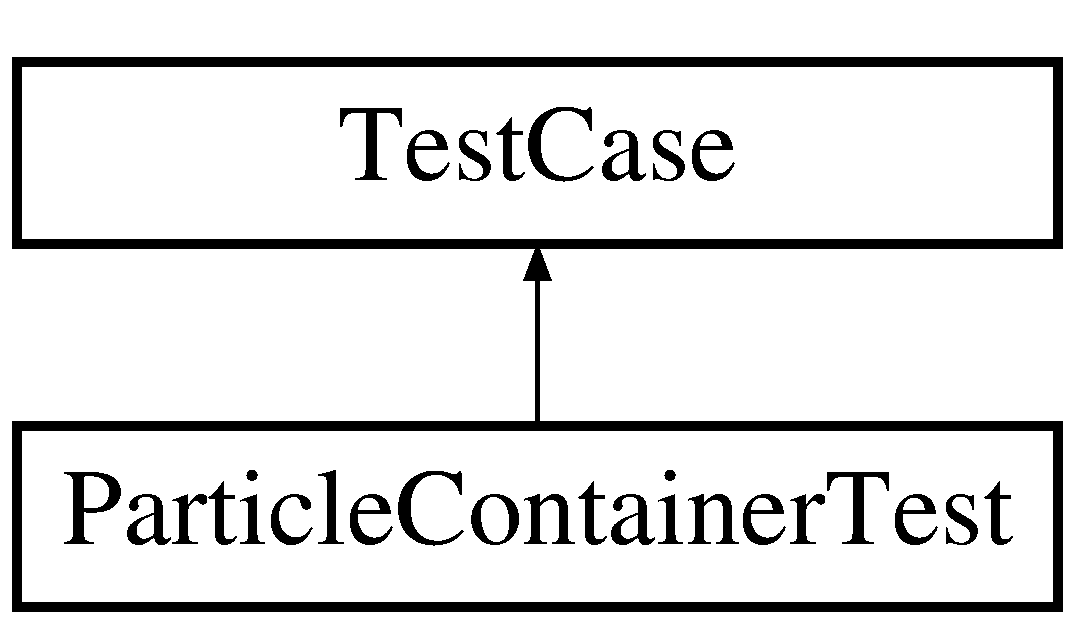
\includegraphics[height=2.000000cm]{classParticleContainerTest}
\end{center}
\end{figure}
\subsection*{Classes}
\begin{DoxyCompactItemize}
\item 
class \hyperlink{classParticleContainerTest_1_1TestHandler}{Test\-Handler}
\item 
struct \hyperlink{structParticleContainerTest_1_1TestParticle}{Test\-Particle}
\end{DoxyCompactItemize}
\subsection*{Public Member Functions}
\begin{DoxyCompactItemize}
\item 
void \hyperlink{classParticleContainerTest_a114674bf106f1237eb8e5d0afa2cead0}{set\-Up} ()
\item 
void \hyperlink{classParticleContainerTest_a3109d4eb4afad3ff4c046fc47ad4fcc4}{tear\-Down} ()
\item 
void \hyperlink{classParticleContainerTest_a60b5dc462c640e3d74a8805faf2b5bbc}{test\-Particle\-Values} ()
\item 
void \hyperlink{classParticleContainerTest_aa5ba7fed4e164c420346f1ddbed066d4}{test\-Particle\-Function} ()
\end{DoxyCompactItemize}
\subsection*{Static Public Member Functions}
\begin{DoxyCompactItemize}
\item 
static Cpp\-Unit\-::\-Test $\ast$ \hyperlink{classParticleContainerTest_a9d826385882d8383f9db17a8265032d3}{suite} ()
\end{DoxyCompactItemize}
\subsection*{Private Attributes}
\begin{DoxyCompactItemize}
\item 
char $\ast$ \hyperlink{classParticleContainerTest_afb8a83e8349f5a068bad149edcc37eb4}{test\-Filename}
\item 
std\-::vector$<$ \hyperlink{structParticleContainerTest_1_1TestParticle}{Test\-Particle} $>$ \hyperlink{classParticleContainerTest_ab6ad3a17d56c5c6d42e0253c56256101}{test\-Particles}
\end{DoxyCompactItemize}


\subsection{Member Function Documentation}
\hypertarget{classParticleContainerTest_a114674bf106f1237eb8e5d0afa2cead0}{\index{Particle\-Container\-Test@{Particle\-Container\-Test}!set\-Up@{set\-Up}}
\index{set\-Up@{set\-Up}!ParticleContainerTest@{Particle\-Container\-Test}}
\subsubsection[{set\-Up}]{\setlength{\rightskip}{0pt plus 5cm}void Particle\-Container\-Test\-::set\-Up (
\begin{DoxyParamCaption}
{}
\end{DoxyParamCaption}
)}}\label{classParticleContainerTest_a114674bf106f1237eb8e5d0afa2cead0}
\hypertarget{classParticleContainerTest_a9d826385882d8383f9db17a8265032d3}{\index{Particle\-Container\-Test@{Particle\-Container\-Test}!suite@{suite}}
\index{suite@{suite}!ParticleContainerTest@{Particle\-Container\-Test}}
\subsubsection[{suite}]{\setlength{\rightskip}{0pt plus 5cm}Test $\ast$ Particle\-Container\-Test\-::suite (
\begin{DoxyParamCaption}
{}
\end{DoxyParamCaption}
)\hspace{0.3cm}{\ttfamily [static]}}}\label{classParticleContainerTest_a9d826385882d8383f9db17a8265032d3}
\hypertarget{classParticleContainerTest_a3109d4eb4afad3ff4c046fc47ad4fcc4}{\index{Particle\-Container\-Test@{Particle\-Container\-Test}!tear\-Down@{tear\-Down}}
\index{tear\-Down@{tear\-Down}!ParticleContainerTest@{Particle\-Container\-Test}}
\subsubsection[{tear\-Down}]{\setlength{\rightskip}{0pt plus 5cm}void Particle\-Container\-Test\-::tear\-Down (
\begin{DoxyParamCaption}
{}
\end{DoxyParamCaption}
)}}\label{classParticleContainerTest_a3109d4eb4afad3ff4c046fc47ad4fcc4}
\hypertarget{classParticleContainerTest_aa5ba7fed4e164c420346f1ddbed066d4}{\index{Particle\-Container\-Test@{Particle\-Container\-Test}!test\-Particle\-Function@{test\-Particle\-Function}}
\index{test\-Particle\-Function@{test\-Particle\-Function}!ParticleContainerTest@{Particle\-Container\-Test}}
\subsubsection[{test\-Particle\-Function}]{\setlength{\rightskip}{0pt plus 5cm}void Particle\-Container\-Test\-::test\-Particle\-Function (
\begin{DoxyParamCaption}
{}
\end{DoxyParamCaption}
)}}\label{classParticleContainerTest_aa5ba7fed4e164c420346f1ddbed066d4}
\hypertarget{classParticleContainerTest_a60b5dc462c640e3d74a8805faf2b5bbc}{\index{Particle\-Container\-Test@{Particle\-Container\-Test}!test\-Particle\-Values@{test\-Particle\-Values}}
\index{test\-Particle\-Values@{test\-Particle\-Values}!ParticleContainerTest@{Particle\-Container\-Test}}
\subsubsection[{test\-Particle\-Values}]{\setlength{\rightskip}{0pt plus 5cm}void Particle\-Container\-Test\-::test\-Particle\-Values (
\begin{DoxyParamCaption}
{}
\end{DoxyParamCaption}
)}}\label{classParticleContainerTest_a60b5dc462c640e3d74a8805faf2b5bbc}


\subsection{Member Data Documentation}
\hypertarget{classParticleContainerTest_afb8a83e8349f5a068bad149edcc37eb4}{\index{Particle\-Container\-Test@{Particle\-Container\-Test}!test\-Filename@{test\-Filename}}
\index{test\-Filename@{test\-Filename}!ParticleContainerTest@{Particle\-Container\-Test}}
\subsubsection[{test\-Filename}]{\setlength{\rightskip}{0pt plus 5cm}char$\ast$ Particle\-Container\-Test\-::test\-Filename\hspace{0.3cm}{\ttfamily [private]}}}\label{classParticleContainerTest_afb8a83e8349f5a068bad149edcc37eb4}
\hypertarget{classParticleContainerTest_ab6ad3a17d56c5c6d42e0253c56256101}{\index{Particle\-Container\-Test@{Particle\-Container\-Test}!test\-Particles@{test\-Particles}}
\index{test\-Particles@{test\-Particles}!ParticleContainerTest@{Particle\-Container\-Test}}
\subsubsection[{test\-Particles}]{\setlength{\rightskip}{0pt plus 5cm}std\-::vector$<${\bf Test\-Particle}$>$ Particle\-Container\-Test\-::test\-Particles\hspace{0.3cm}{\ttfamily [private]}}}\label{classParticleContainerTest_ab6ad3a17d56c5c6d42e0253c56256101}


The documentation for this class was generated from the following files\-:\begin{DoxyCompactItemize}
\item 
src/\hyperlink{UnitTests_8h}{Unit\-Tests.\-h}\item 
src/\hyperlink{UnitTests_8cpp}{Unit\-Tests.\-cpp}\end{DoxyCompactItemize}

\hypertarget{classSimulation_1_1ParticleGenerator}{\section{Simulation\-:\-:Particle\-Generator Class Reference}
\label{classSimulation_1_1ParticleGenerator}\index{Simulation\-::\-Particle\-Generator@{Simulation\-::\-Particle\-Generator}}
}


penerates particles in different shapes  




{\ttfamily \#include $<$Particle\-Generator.\-h$>$}

\subsection*{Static Public Member Functions}
\begin{DoxyCompactItemize}
\item 
static void \hyperlink{classSimulation_1_1ParticleGenerator_a8fb7273c9b825209540396c1cbacf574}{generate\-Cuboid} (\hyperlink{classutils_1_1Vector}{utils\-::\-Vector}$<$ double, 3 $>$ bottom\-Left\-Front, \hyperlink{classutils_1_1Vector}{utils\-::\-Vector}$<$ double, 3 $>$ initial\-Velocity, \hyperlink{classutils_1_1Vector}{utils\-::\-Vector}$<$ int, 3 $>$ num\-Particles, double h, int type, std\-::vector$<$ \hyperlink{classSimulation_1_1Particle}{Particle} $>$ \&particles)
\item 
static void \hyperlink{classSimulation_1_1ParticleGenerator_a1726b3093c82abebf17baf580e5137f4}{generate\-Sphere} (\hyperlink{classutils_1_1Vector}{utils\-::\-Vector}$<$ double, 3 $>$ center, \hyperlink{classutils_1_1Vector}{utils\-::\-Vector}$<$ double, 3 $>$ initial\-Velocity, int num\-Particles, double h, int type, std\-::vector$<$ \hyperlink{classSimulation_1_1Particle}{Particle} $>$ \&particles)
\end{DoxyCompactItemize}


\subsection{Detailed Description}
penerates particles in different shapes 

\subsection{Member Function Documentation}
\hypertarget{classSimulation_1_1ParticleGenerator_a8fb7273c9b825209540396c1cbacf574}{\index{Simulation\-::\-Particle\-Generator@{Simulation\-::\-Particle\-Generator}!generate\-Cuboid@{generate\-Cuboid}}
\index{generate\-Cuboid@{generate\-Cuboid}!Simulation::ParticleGenerator@{Simulation\-::\-Particle\-Generator}}
\subsubsection[{generate\-Cuboid}]{\setlength{\rightskip}{0pt plus 5cm}void Particle\-Generator\-::generate\-Cuboid (
\begin{DoxyParamCaption}
\item[{{\bf utils\-::\-Vector}$<$ double, 3 $>$}]{bottom\-Left\-Front, }
\item[{{\bf utils\-::\-Vector}$<$ double, 3 $>$}]{initial\-Velocity, }
\item[{{\bf utils\-::\-Vector}$<$ int, 3 $>$}]{num\-Particles, }
\item[{double}]{h, }
\item[{int}]{type, }
\item[{std\-::vector$<$ {\bf Particle} $>$ \&}]{particles}
\end{DoxyParamCaption}
)\hspace{0.3cm}{\ttfamily [static]}}}\label{classSimulation_1_1ParticleGenerator_a8fb7273c9b825209540396c1cbacf574}
Generates Cuboid 
\begin{DoxyParams}{Parameters}
{\em bottom\-Left\-Front} & Position of cuboid \\
\hline
{\em num\-Particles} & Number of particles in each axis \\
\hline
{\em initial\-Velocity} & \\
\hline
{\em type} & Type which defines properties of particles \\
\hline
{\em h} & Distance between particles \\
\hline
{\em particles} & List of particles at which cuboid will be apended \\
\hline
\end{DoxyParams}
\hypertarget{classSimulation_1_1ParticleGenerator_a1726b3093c82abebf17baf580e5137f4}{\index{Simulation\-::\-Particle\-Generator@{Simulation\-::\-Particle\-Generator}!generate\-Sphere@{generate\-Sphere}}
\index{generate\-Sphere@{generate\-Sphere}!Simulation::ParticleGenerator@{Simulation\-::\-Particle\-Generator}}
\subsubsection[{generate\-Sphere}]{\setlength{\rightskip}{0pt plus 5cm}void Particle\-Generator\-::generate\-Sphere (
\begin{DoxyParamCaption}
\item[{{\bf utils\-::\-Vector}$<$ double, 3 $>$}]{center, }
\item[{{\bf utils\-::\-Vector}$<$ double, 3 $>$}]{initial\-Velocity, }
\item[{int}]{num\-Particles, }
\item[{double}]{h, }
\item[{int}]{type, }
\item[{std\-::vector$<$ {\bf Particle} $>$ \&}]{particles}
\end{DoxyParamCaption}
)\hspace{0.3cm}{\ttfamily [static]}}}\label{classSimulation_1_1ParticleGenerator_a1726b3093c82abebf17baf580e5137f4}


The documentation for this class was generated from the following files\-:\begin{DoxyCompactItemize}
\item 
src/\hyperlink{ParticleGenerator_8h}{Particle\-Generator.\-h}\item 
src/\hyperlink{ParticleGenerator_8cpp}{Particle\-Generator.\-cpp}\end{DoxyCompactItemize}

\hypertarget{classSimulation_1_1ParticleHandler}{\section{Simulation\-:\-:Particle\-Handler Class Reference}
\label{classSimulation_1_1ParticleHandler}\index{Simulation\-::\-Particle\-Handler@{Simulation\-::\-Particle\-Handler}}
}


{\ttfamily \#include $<$Particle\-Handler.\-h$>$}

Inheritance diagram for Simulation\-:\-:Particle\-Handler\-:\begin{figure}[H]
\begin{center}
\leavevmode
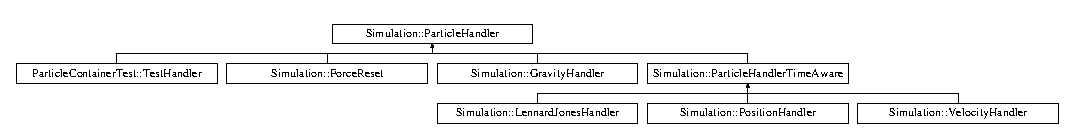
\includegraphics[height=1.794872cm]{classSimulation_1_1ParticleHandler}
\end{center}
\end{figure}
\subsection*{Public Member Functions}
\begin{DoxyCompactItemize}
\item 
virtual void \hyperlink{classSimulation_1_1ParticleHandler_a6b1fc310603bc10093d50c674097fd25}{compute} (\hyperlink{classSimulation_1_1Particle}{Particle} \&p)
\item 
virtual void \hyperlink{classSimulation_1_1ParticleHandler_a013ad557c6892ed2287db090192144ea}{compute} (\hyperlink{classSimulation_1_1Particle}{Particle} \&p1, \hyperlink{classSimulation_1_1Particle}{Particle} \&p2)
\item 
virtual void \hyperlink{classSimulation_1_1ParticleHandler_a4a1caeb40ada4f410fec9244bda4af69}{compute\-Exclusive} (\hyperlink{classSimulation_1_1Particle}{Particle} \&p1, \hyperlink{classSimulation_1_1Particle}{Particle} \&p2)
\end{DoxyCompactItemize}


\subsection{Member Function Documentation}
\hypertarget{classSimulation_1_1ParticleHandler_a6b1fc310603bc10093d50c674097fd25}{\index{Simulation\-::\-Particle\-Handler@{Simulation\-::\-Particle\-Handler}!compute@{compute}}
\index{compute@{compute}!Simulation::ParticleHandler@{Simulation\-::\-Particle\-Handler}}
\subsubsection[{compute}]{\setlength{\rightskip}{0pt plus 5cm}virtual void Simulation\-::\-Particle\-Handler\-::compute (
\begin{DoxyParamCaption}
\item[{{\bf Particle} \&}]{p}
\end{DoxyParamCaption}
)\hspace{0.3cm}{\ttfamily [inline]}, {\ttfamily [virtual]}}}\label{classSimulation_1_1ParticleHandler_a6b1fc310603bc10093d50c674097fd25}


Reimplemented in \hyperlink{classSimulation_1_1LennardJonesHandler_aa2a7d4ce850ece69663918a7cfc4072f}{Simulation\-::\-Lennard\-Jones\-Handler}, \hyperlink{classSimulation_1_1GravityHandler_a7f5b0d36e4e8e3dd6eb54d364add0287}{Simulation\-::\-Gravity\-Handler}, \hyperlink{classSimulation_1_1VelocityHandler_a5ddac3276478a84466bc7bf3e495b6bb}{Simulation\-::\-Velocity\-Handler}, \hyperlink{classSimulation_1_1PositionHandler_adfd177c32d7c11827ae6556ee6dd7602}{Simulation\-::\-Position\-Handler}, and \hyperlink{classParticleContainerTest_1_1TestHandler_a6cb31cb392bac8a4a001a64cefda0634}{Particle\-Container\-Test\-::\-Test\-Handler}.

\hypertarget{classSimulation_1_1ParticleHandler_a013ad557c6892ed2287db090192144ea}{\index{Simulation\-::\-Particle\-Handler@{Simulation\-::\-Particle\-Handler}!compute@{compute}}
\index{compute@{compute}!Simulation::ParticleHandler@{Simulation\-::\-Particle\-Handler}}
\subsubsection[{compute}]{\setlength{\rightskip}{0pt plus 5cm}virtual void Simulation\-::\-Particle\-Handler\-::compute (
\begin{DoxyParamCaption}
\item[{{\bf Particle} \&}]{p1, }
\item[{{\bf Particle} \&}]{p2}
\end{DoxyParamCaption}
)\hspace{0.3cm}{\ttfamily [inline]}, {\ttfamily [virtual]}}}\label{classSimulation_1_1ParticleHandler_a013ad557c6892ed2287db090192144ea}


Reimplemented in \hyperlink{classSimulation_1_1LennardJonesHandler_a81842168e68a61cb75448f91bc27f99c}{Simulation\-::\-Lennard\-Jones\-Handler}, and \hyperlink{classSimulation_1_1GravityHandler_a7805aa1b40a206d9fe3362a321d933ed}{Simulation\-::\-Gravity\-Handler}.

\hypertarget{classSimulation_1_1ParticleHandler_a4a1caeb40ada4f410fec9244bda4af69}{\index{Simulation\-::\-Particle\-Handler@{Simulation\-::\-Particle\-Handler}!compute\-Exclusive@{compute\-Exclusive}}
\index{compute\-Exclusive@{compute\-Exclusive}!Simulation::ParticleHandler@{Simulation\-::\-Particle\-Handler}}
\subsubsection[{compute\-Exclusive}]{\setlength{\rightskip}{0pt plus 5cm}virtual void Simulation\-::\-Particle\-Handler\-::compute\-Exclusive (
\begin{DoxyParamCaption}
\item[{{\bf Particle} \&}]{p1, }
\item[{{\bf Particle} \&}]{p2}
\end{DoxyParamCaption}
)\hspace{0.3cm}{\ttfamily [inline]}, {\ttfamily [virtual]}}}\label{classSimulation_1_1ParticleHandler_a4a1caeb40ada4f410fec9244bda4af69}


Reimplemented in \hyperlink{classSimulation_1_1LennardJonesHandler_ac16127a588f6e8598dc2598d1224517f}{Simulation\-::\-Lennard\-Jones\-Handler}, and \hyperlink{classSimulation_1_1GravityHandler_a4abb48d878ea825e6582ba0bf9ae5c0d}{Simulation\-::\-Gravity\-Handler}.



The documentation for this class was generated from the following file\-:\begin{DoxyCompactItemize}
\item 
src/\hyperlink{ParticleHandler_8h}{Particle\-Handler.\-h}\end{DoxyCompactItemize}

\hypertarget{classSimulation_1_1ParticleHandlerTimeAware}{\section{Simulation\-:\-:Particle\-Handler\-Time\-Aware Class Reference}
\label{classSimulation_1_1ParticleHandlerTimeAware}\index{Simulation\-::\-Particle\-Handler\-Time\-Aware@{Simulation\-::\-Particle\-Handler\-Time\-Aware}}
}


{\ttfamily \#include $<$Particle\-Handler.\-h$>$}

Inheritance diagram for Simulation\-:\-:Particle\-Handler\-Time\-Aware\-:\begin{figure}[H]
\begin{center}
\leavevmode
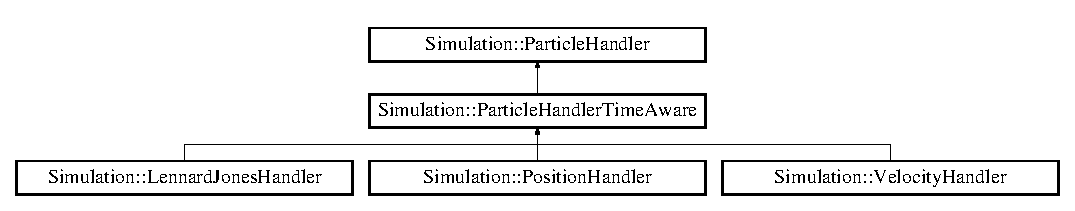
\includegraphics[height=1.794872cm]{classSimulation_1_1ParticleHandlerTimeAware}
\end{center}
\end{figure}
\subsection*{Public Member Functions}
\begin{DoxyCompactItemize}
\item 
\hyperlink{classSimulation_1_1ParticleHandlerTimeAware_a839536b59b78947066e2b9cbf01010fc}{Particle\-Handler\-Time\-Aware} (double dt)
\end{DoxyCompactItemize}
\subsection*{Protected Attributes}
\begin{DoxyCompactItemize}
\item 
double \hyperlink{classSimulation_1_1ParticleHandlerTimeAware_a8c6378b506877c8d69dee8c31f3dfc45}{delta\-\_\-t}
\end{DoxyCompactItemize}


\subsection{Constructor \& Destructor Documentation}
\hypertarget{classSimulation_1_1ParticleHandlerTimeAware_a839536b59b78947066e2b9cbf01010fc}{\index{Simulation\-::\-Particle\-Handler\-Time\-Aware@{Simulation\-::\-Particle\-Handler\-Time\-Aware}!Particle\-Handler\-Time\-Aware@{Particle\-Handler\-Time\-Aware}}
\index{Particle\-Handler\-Time\-Aware@{Particle\-Handler\-Time\-Aware}!Simulation::ParticleHandlerTimeAware@{Simulation\-::\-Particle\-Handler\-Time\-Aware}}
\subsubsection[{Particle\-Handler\-Time\-Aware}]{\setlength{\rightskip}{0pt plus 5cm}Simulation\-::\-Particle\-Handler\-Time\-Aware\-::\-Particle\-Handler\-Time\-Aware (
\begin{DoxyParamCaption}
\item[{double}]{dt}
\end{DoxyParamCaption}
)\hspace{0.3cm}{\ttfamily [inline]}}}\label{classSimulation_1_1ParticleHandlerTimeAware_a839536b59b78947066e2b9cbf01010fc}


\subsection{Member Data Documentation}
\hypertarget{classSimulation_1_1ParticleHandlerTimeAware_a8c6378b506877c8d69dee8c31f3dfc45}{\index{Simulation\-::\-Particle\-Handler\-Time\-Aware@{Simulation\-::\-Particle\-Handler\-Time\-Aware}!delta\-\_\-t@{delta\-\_\-t}}
\index{delta\-\_\-t@{delta\-\_\-t}!Simulation::ParticleHandlerTimeAware@{Simulation\-::\-Particle\-Handler\-Time\-Aware}}
\subsubsection[{delta\-\_\-t}]{\setlength{\rightskip}{0pt plus 5cm}double Simulation\-::\-Particle\-Handler\-Time\-Aware\-::delta\-\_\-t\hspace{0.3cm}{\ttfamily [protected]}}}\label{classSimulation_1_1ParticleHandlerTimeAware_a8c6378b506877c8d69dee8c31f3dfc45}


The documentation for this class was generated from the following file\-:\begin{DoxyCompactItemize}
\item 
src/\hyperlink{ParticleHandler_8h}{Particle\-Handler.\-h}\end{DoxyCompactItemize}

\hypertarget{classSimulation_1_1ParticleProperty}{\section{Simulation\-:\-:Particle\-Property Class Reference}
\label{classSimulation_1_1ParticleProperty}\index{Simulation\-::\-Particle\-Property@{Simulation\-::\-Particle\-Property}}
}


Stores properties for one type of particles.  




{\ttfamily \#include $<$Particle.\-h$>$}

\subsection*{Public Member Functions}
\begin{DoxyCompactItemize}
\item 
\hyperlink{classSimulation_1_1ParticleProperty_a6a931af7787ba8bb7ee3bba88cc875e6}{Particle\-Property} ()
\begin{DoxyCompactList}\small\item\em Contructor for property. \end{DoxyCompactList}\end{DoxyCompactItemize}
\subsection*{Static Public Member Functions}
\begin{DoxyCompactItemize}
\item 
static void \hyperlink{classSimulation_1_1ParticleProperty_af725f9c9d30cb1b64fe669a7842de12c}{push} (\hyperlink{classSimulation_1_1ParticleProperty}{Particle\-Property} \&prop)
\begin{DoxyCompactList}\small\item\em Add new type of particles. \end{DoxyCompactList}\item 
static \hyperlink{classSimulation_1_1ParticleProperty}{Particle\-Property} \& \hyperlink{classSimulation_1_1ParticleProperty_acab370093ec1ad31402b68aaf386dad2}{get} (int i)
\item 
static int \hyperlink{classSimulation_1_1ParticleProperty_a000e6d8061005aa0352ad66d97e41efc}{count} ()
\end{DoxyCompactItemize}
\subsection*{Public Attributes}
\begin{DoxyCompactItemize}
\item 
double \hyperlink{classSimulation_1_1ParticleProperty_a8f145877445ca59f131da94402d2f754}{mass}
\begin{DoxyCompactList}\small\item\em Mass of particle. \end{DoxyCompactList}\item 
double \hyperlink{classSimulation_1_1ParticleProperty_a3b5090b0388ea6708f204377648b9f7d}{e}
\begin{DoxyCompactList}\small\item\em Epsilon of particle. \end{DoxyCompactList}\item 
double \hyperlink{classSimulation_1_1ParticleProperty_a53851810b9a7de47591967ce60b69367}{o}
\begin{DoxyCompactList}\small\item\em Sigma of particle. \end{DoxyCompactList}\end{DoxyCompactItemize}
\subsection*{Static Private Attributes}
\begin{DoxyCompactItemize}
\item 
static std\-::vector\\*
$<$ \hyperlink{classSimulation_1_1ParticleProperty}{Particle\-Property} $>$ \hyperlink{classSimulation_1_1ParticleProperty_a347c0996e25e4d4fa48ca1ce3db7e7f7}{properties}
\begin{DoxyCompactList}\small\item\em list of all type properties \end{DoxyCompactList}\end{DoxyCompactItemize}


\subsection{Detailed Description}
Stores properties for one type of particles. 

\subsection{Constructor \& Destructor Documentation}
\hypertarget{classSimulation_1_1ParticleProperty_a6a931af7787ba8bb7ee3bba88cc875e6}{\index{Simulation\-::\-Particle\-Property@{Simulation\-::\-Particle\-Property}!Particle\-Property@{Particle\-Property}}
\index{Particle\-Property@{Particle\-Property}!Simulation::ParticleProperty@{Simulation\-::\-Particle\-Property}}
\subsubsection[{Particle\-Property}]{\setlength{\rightskip}{0pt plus 5cm}Simulation\-::\-Particle\-Property\-::\-Particle\-Property (
\begin{DoxyParamCaption}
{}
\end{DoxyParamCaption}
)\hspace{0.3cm}{\ttfamily [inline]}}}\label{classSimulation_1_1ParticleProperty_a6a931af7787ba8bb7ee3bba88cc875e6}


Contructor for property. 



\subsection{Member Function Documentation}
\hypertarget{classSimulation_1_1ParticleProperty_a000e6d8061005aa0352ad66d97e41efc}{\index{Simulation\-::\-Particle\-Property@{Simulation\-::\-Particle\-Property}!count@{count}}
\index{count@{count}!Simulation::ParticleProperty@{Simulation\-::\-Particle\-Property}}
\subsubsection[{count}]{\setlength{\rightskip}{0pt plus 5cm}int Particle\-Property\-::count (
\begin{DoxyParamCaption}
{}
\end{DoxyParamCaption}
)\hspace{0.3cm}{\ttfamily [static]}}}\label{classSimulation_1_1ParticleProperty_a000e6d8061005aa0352ad66d97e41efc}
\begin{DoxyReturn}{Returns}
Number of properties 
\end{DoxyReturn}
\hypertarget{classSimulation_1_1ParticleProperty_acab370093ec1ad31402b68aaf386dad2}{\index{Simulation\-::\-Particle\-Property@{Simulation\-::\-Particle\-Property}!get@{get}}
\index{get@{get}!Simulation::ParticleProperty@{Simulation\-::\-Particle\-Property}}
\subsubsection[{get}]{\setlength{\rightskip}{0pt plus 5cm}{\bf Particle\-Property} \& Particle\-Property\-::get (
\begin{DoxyParamCaption}
\item[{int}]{i}
\end{DoxyParamCaption}
)\hspace{0.3cm}{\ttfamily [static]}}}\label{classSimulation_1_1ParticleProperty_acab370093ec1ad31402b68aaf386dad2}
Get properties for type 
\begin{DoxyParams}{Parameters}
{\em i} & Type of particle \\
\hline
\end{DoxyParams}
\hypertarget{classSimulation_1_1ParticleProperty_af725f9c9d30cb1b64fe669a7842de12c}{\index{Simulation\-::\-Particle\-Property@{Simulation\-::\-Particle\-Property}!push@{push}}
\index{push@{push}!Simulation::ParticleProperty@{Simulation\-::\-Particle\-Property}}
\subsubsection[{push}]{\setlength{\rightskip}{0pt plus 5cm}void Particle\-Property\-::push (
\begin{DoxyParamCaption}
\item[{{\bf Particle\-Property} \&}]{prop}
\end{DoxyParamCaption}
)\hspace{0.3cm}{\ttfamily [static]}}}\label{classSimulation_1_1ParticleProperty_af725f9c9d30cb1b64fe669a7842de12c}


Add new type of particles. 



\subsection{Member Data Documentation}
\hypertarget{classSimulation_1_1ParticleProperty_a3b5090b0388ea6708f204377648b9f7d}{\index{Simulation\-::\-Particle\-Property@{Simulation\-::\-Particle\-Property}!e@{e}}
\index{e@{e}!Simulation::ParticleProperty@{Simulation\-::\-Particle\-Property}}
\subsubsection[{e}]{\setlength{\rightskip}{0pt plus 5cm}double Simulation\-::\-Particle\-Property\-::e}}\label{classSimulation_1_1ParticleProperty_a3b5090b0388ea6708f204377648b9f7d}


Epsilon of particle. 

\begin{DoxyNote}{Note}
Used for Lennard-\/\-Jones potential 
\end{DoxyNote}
\hypertarget{classSimulation_1_1ParticleProperty_a8f145877445ca59f131da94402d2f754}{\index{Simulation\-::\-Particle\-Property@{Simulation\-::\-Particle\-Property}!mass@{mass}}
\index{mass@{mass}!Simulation::ParticleProperty@{Simulation\-::\-Particle\-Property}}
\subsubsection[{mass}]{\setlength{\rightskip}{0pt plus 5cm}double Simulation\-::\-Particle\-Property\-::mass}}\label{classSimulation_1_1ParticleProperty_a8f145877445ca59f131da94402d2f754}


Mass of particle. 

\hypertarget{classSimulation_1_1ParticleProperty_a53851810b9a7de47591967ce60b69367}{\index{Simulation\-::\-Particle\-Property@{Simulation\-::\-Particle\-Property}!o@{o}}
\index{o@{o}!Simulation::ParticleProperty@{Simulation\-::\-Particle\-Property}}
\subsubsection[{o}]{\setlength{\rightskip}{0pt plus 5cm}double Simulation\-::\-Particle\-Property\-::o}}\label{classSimulation_1_1ParticleProperty_a53851810b9a7de47591967ce60b69367}


Sigma of particle. 

\begin{DoxyNote}{Note}
Used for Lennard-\/\-Jones potential 
\end{DoxyNote}
\hypertarget{classSimulation_1_1ParticleProperty_a347c0996e25e4d4fa48ca1ce3db7e7f7}{\index{Simulation\-::\-Particle\-Property@{Simulation\-::\-Particle\-Property}!properties@{properties}}
\index{properties@{properties}!Simulation::ParticleProperty@{Simulation\-::\-Particle\-Property}}
\subsubsection[{properties}]{\setlength{\rightskip}{0pt plus 5cm}vector$<$ {\bf Particle\-Property} $>$ Particle\-Property\-::properties\hspace{0.3cm}{\ttfamily [static]}, {\ttfamily [private]}}}\label{classSimulation_1_1ParticleProperty_a347c0996e25e4d4fa48ca1ce3db7e7f7}


list of all type properties 



The documentation for this class was generated from the following files\-:\begin{DoxyCompactItemize}
\item 
src/\hyperlink{Particle_8h}{Particle.\-h}\item 
src/\hyperlink{Particle_8cpp}{Particle.\-cpp}\end{DoxyCompactItemize}

\hypertarget{classSimulation_1_1PositionHandler}{\section{Simulation\-:\-:Position\-Handler Class Reference}
\label{classSimulation_1_1PositionHandler}\index{Simulation\-::\-Position\-Handler@{Simulation\-::\-Position\-Handler}}
}


{\ttfamily \#include $<$Particle\-Handler.\-h$>$}

Inheritance diagram for Simulation\-:\-:Position\-Handler\-:\begin{figure}[H]
\begin{center}
\leavevmode
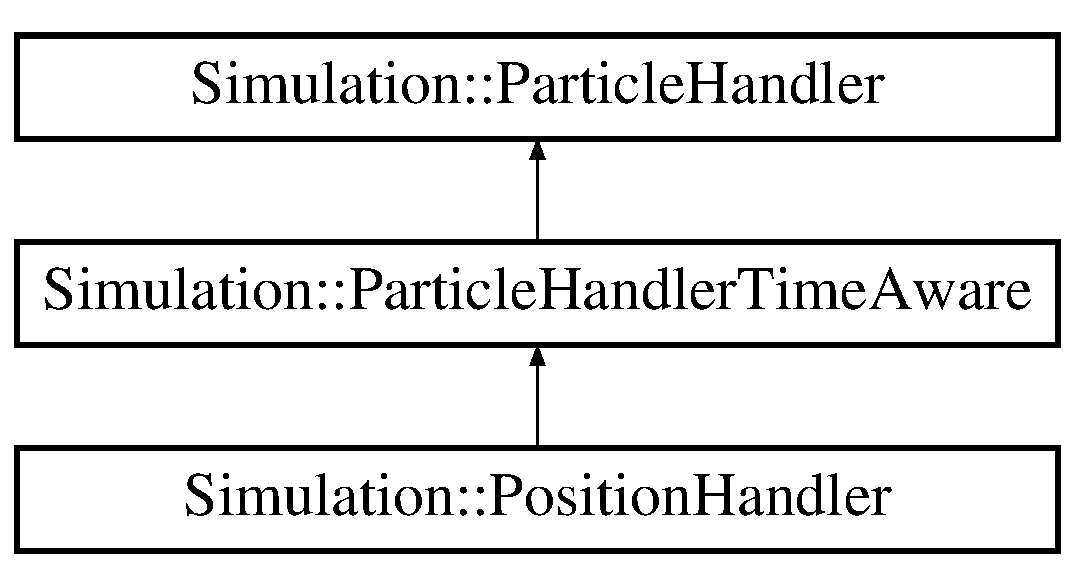
\includegraphics[height=3.000000cm]{classSimulation_1_1PositionHandler}
\end{center}
\end{figure}
\subsection*{Public Member Functions}
\begin{DoxyCompactItemize}
\item 
\hyperlink{classSimulation_1_1PositionHandler_ab66e6345c9e20bae0fc297253e4f6f5f}{Position\-Handler} (double dt)
\item 
void \hyperlink{classSimulation_1_1PositionHandler_adfd177c32d7c11827ae6556ee6dd7602}{compute} (\hyperlink{classSimulation_1_1Particle}{Particle} \&p)
\end{DoxyCompactItemize}
\subsection*{Additional Inherited Members}


\subsection{Constructor \& Destructor Documentation}
\hypertarget{classSimulation_1_1PositionHandler_ab66e6345c9e20bae0fc297253e4f6f5f}{\index{Simulation\-::\-Position\-Handler@{Simulation\-::\-Position\-Handler}!Position\-Handler@{Position\-Handler}}
\index{Position\-Handler@{Position\-Handler}!Simulation::PositionHandler@{Simulation\-::\-Position\-Handler}}
\subsubsection[{Position\-Handler}]{\setlength{\rightskip}{0pt plus 5cm}Simulation\-::\-Position\-Handler\-::\-Position\-Handler (
\begin{DoxyParamCaption}
\item[{double}]{dt}
\end{DoxyParamCaption}
)\hspace{0.3cm}{\ttfamily [inline]}}}\label{classSimulation_1_1PositionHandler_ab66e6345c9e20bae0fc297253e4f6f5f}


\subsection{Member Function Documentation}
\hypertarget{classSimulation_1_1PositionHandler_adfd177c32d7c11827ae6556ee6dd7602}{\index{Simulation\-::\-Position\-Handler@{Simulation\-::\-Position\-Handler}!compute@{compute}}
\index{compute@{compute}!Simulation::PositionHandler@{Simulation\-::\-Position\-Handler}}
\subsubsection[{compute}]{\setlength{\rightskip}{0pt plus 5cm}void Simulation\-::\-Position\-Handler\-::compute (
\begin{DoxyParamCaption}
\item[{{\bf Particle} \&}]{p}
\end{DoxyParamCaption}
)\hspace{0.3cm}{\ttfamily [inline]}, {\ttfamily [virtual]}}}\label{classSimulation_1_1PositionHandler_adfd177c32d7c11827ae6556ee6dd7602}


Reimplemented from \hyperlink{classSimulation_1_1ParticleHandler_a6b1fc310603bc10093d50c674097fd25}{Simulation\-::\-Particle\-Handler}.



The documentation for this class was generated from the following file\-:\begin{DoxyCompactItemize}
\item 
src/\hyperlink{ParticleHandler_8h}{Particle\-Handler.\-h}\end{DoxyCompactItemize}

\hypertarget{classSimulation_1_1StateWriter}{\section{Simulation\-:\-:State\-Writer Class Reference}
\label{classSimulation_1_1StateWriter}\index{Simulation\-::\-State\-Writer@{Simulation\-::\-State\-Writer}}
}


{\ttfamily \#include $<$State\-Writer.\-h$>$}

\subsection*{Static Public Member Functions}
\begin{DoxyCompactItemize}
\item 
static void \hyperlink{classSimulation_1_1StateWriter_a75003a7abe17ba5a0b181e28c227398a}{write\-State\-To\-File} (const char $\ast$filename, \hyperlink{classSimulation_1_1ParticleContainer}{Particle\-Container} \&\hyperlink{MolSim_8cpp_ab06a8478b206d59f33b5b4a630c3804e}{container})
\end{DoxyCompactItemize}


\subsection{Member Function Documentation}
\hypertarget{classSimulation_1_1StateWriter_a75003a7abe17ba5a0b181e28c227398a}{\index{Simulation\-::\-State\-Writer@{Simulation\-::\-State\-Writer}!write\-State\-To\-File@{write\-State\-To\-File}}
\index{write\-State\-To\-File@{write\-State\-To\-File}!Simulation::StateWriter@{Simulation\-::\-State\-Writer}}
\subsubsection[{write\-State\-To\-File}]{\setlength{\rightskip}{0pt plus 5cm}void State\-Writer\-::write\-State\-To\-File (
\begin{DoxyParamCaption}
\item[{const char $\ast$}]{filename, }
\item[{{\bf Particle\-Container} \&}]{container}
\end{DoxyParamCaption}
)\hspace{0.3cm}{\ttfamily [static]}}}\label{classSimulation_1_1StateWriter_a75003a7abe17ba5a0b181e28c227398a}


The documentation for this class was generated from the following files\-:\begin{DoxyCompactItemize}
\item 
src/\hyperlink{StateWriter_8h}{State\-Writer.\-h}\item 
src/\hyperlink{StateWriter_8cpp}{State\-Writer.\-cpp}\end{DoxyCompactItemize}

\hypertarget{classParticleContainerTest_1_1TestHandler}{\section{Particle\-Container\-Test\-:\-:Test\-Handler Class Reference}
\label{classParticleContainerTest_1_1TestHandler}\index{Particle\-Container\-Test\-::\-Test\-Handler@{Particle\-Container\-Test\-::\-Test\-Handler}}
}
Inheritance diagram for Particle\-Container\-Test\-:\-:Test\-Handler\-:\begin{figure}[H]
\begin{center}
\leavevmode
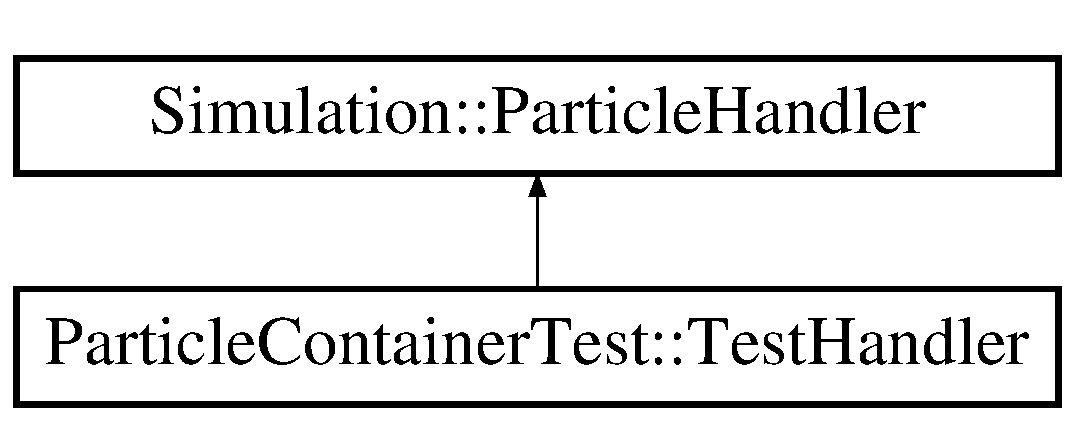
\includegraphics[height=2.000000cm]{classParticleContainerTest_1_1TestHandler}
\end{center}
\end{figure}
\subsection*{Public Member Functions}
\begin{DoxyCompactItemize}
\item 
void \hyperlink{classParticleContainerTest_1_1TestHandler_a6cb31cb392bac8a4a001a64cefda0634}{compute} (\hyperlink{classSimulation_1_1Particle}{Simulation\-::\-Particle} \&p)
\begin{DoxyCompactList}\small\item\em Computes one single particle. \end{DoxyCompactList}\end{DoxyCompactItemize}


\subsection{Member Function Documentation}
\hypertarget{classParticleContainerTest_1_1TestHandler_a6cb31cb392bac8a4a001a64cefda0634}{\index{Particle\-Container\-Test\-::\-Test\-Handler@{Particle\-Container\-Test\-::\-Test\-Handler}!compute@{compute}}
\index{compute@{compute}!ParticleContainerTest::TestHandler@{Particle\-Container\-Test\-::\-Test\-Handler}}
\subsubsection[{compute}]{\setlength{\rightskip}{0pt plus 5cm}void Particle\-Container\-Test\-::\-Test\-Handler\-::compute (
\begin{DoxyParamCaption}
\item[{{\bf Simulation\-::\-Particle} \&}]{p}
\end{DoxyParamCaption}
)\hspace{0.3cm}{\ttfamily [inline]}, {\ttfamily [virtual]}}}\label{classParticleContainerTest_1_1TestHandler_a6cb31cb392bac8a4a001a64cefda0634}


Computes one single particle. 



Reimplemented from \hyperlink{classSimulation_1_1ParticleHandler_a6b1fc310603bc10093d50c674097fd25}{Simulation\-::\-Particle\-Handler}.



The documentation for this class was generated from the following file\-:\begin{DoxyCompactItemize}
\item 
src/\hyperlink{UnitTests_8h}{Unit\-Tests.\-h}\end{DoxyCompactItemize}

\hypertarget{structParticleContainerTest_1_1TestParticle}{\section{Particle\-Container\-Test\-:\-:Test\-Particle Struct Reference}
\label{structParticleContainerTest_1_1TestParticle}\index{Particle\-Container\-Test\-::\-Test\-Particle@{Particle\-Container\-Test\-::\-Test\-Particle}}
}
\subsection*{Public Attributes}
\begin{DoxyCompactItemize}
\item 
double \hyperlink{structParticleContainerTest_1_1TestParticle_add0472ca8a31ba4630b5470fc710fd37}{x}
\item 
double \hyperlink{structParticleContainerTest_1_1TestParticle_af27fbca6e49c80bd1b8555df0e7b1380}{y}
\item 
double \hyperlink{structParticleContainerTest_1_1TestParticle_a0d9bef972bdcf0fc2465aa2a4d124033}{z}
\item 
double \hyperlink{structParticleContainerTest_1_1TestParticle_aa99b7d2fe342a22534ce92585441bbd3}{vx}
\item 
double \hyperlink{structParticleContainerTest_1_1TestParticle_aa0f006f1d60465699bdb74f5716cd1f2}{vy}
\item 
double \hyperlink{structParticleContainerTest_1_1TestParticle_a262ea711c8f55a21404fa62401933c6b}{vz}
\item 
double \hyperlink{structParticleContainerTest_1_1TestParticle_af110e6ebdcce198c96cf93cce206dd6c}{m}
\end{DoxyCompactItemize}


\subsection{Member Data Documentation}
\hypertarget{structParticleContainerTest_1_1TestParticle_af110e6ebdcce198c96cf93cce206dd6c}{\index{Particle\-Container\-Test\-::\-Test\-Particle@{Particle\-Container\-Test\-::\-Test\-Particle}!m@{m}}
\index{m@{m}!ParticleContainerTest::TestParticle@{Particle\-Container\-Test\-::\-Test\-Particle}}
\subsubsection[{m}]{\setlength{\rightskip}{0pt plus 5cm}double Particle\-Container\-Test\-::\-Test\-Particle\-::m}}\label{structParticleContainerTest_1_1TestParticle_af110e6ebdcce198c96cf93cce206dd6c}
\hypertarget{structParticleContainerTest_1_1TestParticle_aa99b7d2fe342a22534ce92585441bbd3}{\index{Particle\-Container\-Test\-::\-Test\-Particle@{Particle\-Container\-Test\-::\-Test\-Particle}!vx@{vx}}
\index{vx@{vx}!ParticleContainerTest::TestParticle@{Particle\-Container\-Test\-::\-Test\-Particle}}
\subsubsection[{vx}]{\setlength{\rightskip}{0pt plus 5cm}double Particle\-Container\-Test\-::\-Test\-Particle\-::vx}}\label{structParticleContainerTest_1_1TestParticle_aa99b7d2fe342a22534ce92585441bbd3}
\hypertarget{structParticleContainerTest_1_1TestParticle_aa0f006f1d60465699bdb74f5716cd1f2}{\index{Particle\-Container\-Test\-::\-Test\-Particle@{Particle\-Container\-Test\-::\-Test\-Particle}!vy@{vy}}
\index{vy@{vy}!ParticleContainerTest::TestParticle@{Particle\-Container\-Test\-::\-Test\-Particle}}
\subsubsection[{vy}]{\setlength{\rightskip}{0pt plus 5cm}double Particle\-Container\-Test\-::\-Test\-Particle\-::vy}}\label{structParticleContainerTest_1_1TestParticle_aa0f006f1d60465699bdb74f5716cd1f2}
\hypertarget{structParticleContainerTest_1_1TestParticle_a262ea711c8f55a21404fa62401933c6b}{\index{Particle\-Container\-Test\-::\-Test\-Particle@{Particle\-Container\-Test\-::\-Test\-Particle}!vz@{vz}}
\index{vz@{vz}!ParticleContainerTest::TestParticle@{Particle\-Container\-Test\-::\-Test\-Particle}}
\subsubsection[{vz}]{\setlength{\rightskip}{0pt plus 5cm}double Particle\-Container\-Test\-::\-Test\-Particle\-::vz}}\label{structParticleContainerTest_1_1TestParticle_a262ea711c8f55a21404fa62401933c6b}
\hypertarget{structParticleContainerTest_1_1TestParticle_add0472ca8a31ba4630b5470fc710fd37}{\index{Particle\-Container\-Test\-::\-Test\-Particle@{Particle\-Container\-Test\-::\-Test\-Particle}!x@{x}}
\index{x@{x}!ParticleContainerTest::TestParticle@{Particle\-Container\-Test\-::\-Test\-Particle}}
\subsubsection[{x}]{\setlength{\rightskip}{0pt plus 5cm}double Particle\-Container\-Test\-::\-Test\-Particle\-::x}}\label{structParticleContainerTest_1_1TestParticle_add0472ca8a31ba4630b5470fc710fd37}
\hypertarget{structParticleContainerTest_1_1TestParticle_af27fbca6e49c80bd1b8555df0e7b1380}{\index{Particle\-Container\-Test\-::\-Test\-Particle@{Particle\-Container\-Test\-::\-Test\-Particle}!y@{y}}
\index{y@{y}!ParticleContainerTest::TestParticle@{Particle\-Container\-Test\-::\-Test\-Particle}}
\subsubsection[{y}]{\setlength{\rightskip}{0pt plus 5cm}double Particle\-Container\-Test\-::\-Test\-Particle\-::y}}\label{structParticleContainerTest_1_1TestParticle_af27fbca6e49c80bd1b8555df0e7b1380}
\hypertarget{structParticleContainerTest_1_1TestParticle_a0d9bef972bdcf0fc2465aa2a4d124033}{\index{Particle\-Container\-Test\-::\-Test\-Particle@{Particle\-Container\-Test\-::\-Test\-Particle}!z@{z}}
\index{z@{z}!ParticleContainerTest::TestParticle@{Particle\-Container\-Test\-::\-Test\-Particle}}
\subsubsection[{z}]{\setlength{\rightskip}{0pt plus 5cm}double Particle\-Container\-Test\-::\-Test\-Particle\-::z}}\label{structParticleContainerTest_1_1TestParticle_a0d9bef972bdcf0fc2465aa2a4d124033}


The documentation for this struct was generated from the following file\-:\begin{DoxyCompactItemize}
\item 
src/\hyperlink{UnitTests_8h}{Unit\-Tests.\-h}\end{DoxyCompactItemize}

\hypertarget{classSimulation_1_1Thermostat}{\section{Simulation\-:\-:Thermostat Class Reference}
\label{classSimulation_1_1Thermostat}\index{Simulation\-::\-Thermostat@{Simulation\-::\-Thermostat}}
}


Handles temperature of particles in the simulation.  




{\ttfamily \#include $<$Thermostat.\-h$>$}

\subsection*{Public Member Functions}
\begin{DoxyCompactItemize}
\item 
\hyperlink{classSimulation_1_1Thermostat_a3132362562357ff26f7bb02fa9ed59e0}{Thermostat} (\hyperlink{classSimulation_1_1ParticleContainer}{Particle\-Container} \&cont)
\item 
void \hyperlink{classSimulation_1_1Thermostat_a6d7ef0a0e8dc0aadee57630d63938f7d}{scale\-Temperature} (double scaling)
\begin{DoxyCompactList}\small\item\em Scale temperature of simulation. \end{DoxyCompactList}\item 
double \hyperlink{classSimulation_1_1Thermostat_ac082f2cc212aa2ac0c7d364e96afdb32}{calc\-Kinetic\-Energy} ()
\begin{DoxyCompactList}\small\item\em Calculate kinetic energy of simulation. \end{DoxyCompactList}\item 
void \hyperlink{classSimulation_1_1Thermostat_adac7020482a6f258d5d4757099016c22}{apply\-Temperature} (double temp)
\begin{DoxyCompactList}\small\item\em Apply temperature to simulation. \end{DoxyCompactList}\item 
void \hyperlink{classSimulation_1_1Thermostat_a37f1ec4f15eaeb89580d3fd28a0c984f}{apply\-Initial\-Temperature} (double temp)
\begin{DoxyCompactList}\small\item\em Apply initial temperature to simulation. \end{DoxyCompactList}\end{DoxyCompactItemize}
\subsection*{Private Attributes}
\begin{DoxyCompactItemize}
\item 
\hyperlink{classSimulation_1_1ParticleContainer}{Particle\-Container} \& \hyperlink{classSimulation_1_1Thermostat_a7625bc9f97f3b385ec28a4e049898032}{container}
\begin{DoxyCompactList}\small\item\em Container which stores particles for temperature calculations. \end{DoxyCompactList}\end{DoxyCompactItemize}


\subsection{Detailed Description}
Handles temperature of particles in the simulation. 

\subsection{Constructor \& Destructor Documentation}
\hypertarget{classSimulation_1_1Thermostat_a3132362562357ff26f7bb02fa9ed59e0}{\index{Simulation\-::\-Thermostat@{Simulation\-::\-Thermostat}!Thermostat@{Thermostat}}
\index{Thermostat@{Thermostat}!Simulation::Thermostat@{Simulation\-::\-Thermostat}}
\subsubsection[{Thermostat}]{\setlength{\rightskip}{0pt plus 5cm}Thermostat\-::\-Thermostat (
\begin{DoxyParamCaption}
\item[{{\bf Particle\-Container} \&}]{cont}
\end{DoxyParamCaption}
)}}\label{classSimulation_1_1Thermostat_a3132362562357ff26f7bb02fa9ed59e0}


\subsection{Member Function Documentation}
\hypertarget{classSimulation_1_1Thermostat_a37f1ec4f15eaeb89580d3fd28a0c984f}{\index{Simulation\-::\-Thermostat@{Simulation\-::\-Thermostat}!apply\-Initial\-Temperature@{apply\-Initial\-Temperature}}
\index{apply\-Initial\-Temperature@{apply\-Initial\-Temperature}!Simulation::Thermostat@{Simulation\-::\-Thermostat}}
\subsubsection[{apply\-Initial\-Temperature}]{\setlength{\rightskip}{0pt plus 5cm}void Thermostat\-::apply\-Initial\-Temperature (
\begin{DoxyParamCaption}
\item[{double}]{temp}
\end{DoxyParamCaption}
)}}\label{classSimulation_1_1Thermostat_a37f1ec4f15eaeb89580d3fd28a0c984f}


Apply initial temperature to simulation. 

\hypertarget{classSimulation_1_1Thermostat_adac7020482a6f258d5d4757099016c22}{\index{Simulation\-::\-Thermostat@{Simulation\-::\-Thermostat}!apply\-Temperature@{apply\-Temperature}}
\index{apply\-Temperature@{apply\-Temperature}!Simulation::Thermostat@{Simulation\-::\-Thermostat}}
\subsubsection[{apply\-Temperature}]{\setlength{\rightskip}{0pt plus 5cm}void Thermostat\-::apply\-Temperature (
\begin{DoxyParamCaption}
\item[{double}]{temp}
\end{DoxyParamCaption}
)}}\label{classSimulation_1_1Thermostat_adac7020482a6f258d5d4757099016c22}


Apply temperature to simulation. 

\hypertarget{classSimulation_1_1Thermostat_ac082f2cc212aa2ac0c7d364e96afdb32}{\index{Simulation\-::\-Thermostat@{Simulation\-::\-Thermostat}!calc\-Kinetic\-Energy@{calc\-Kinetic\-Energy}}
\index{calc\-Kinetic\-Energy@{calc\-Kinetic\-Energy}!Simulation::Thermostat@{Simulation\-::\-Thermostat}}
\subsubsection[{calc\-Kinetic\-Energy}]{\setlength{\rightskip}{0pt plus 5cm}double Thermostat\-::calc\-Kinetic\-Energy (
\begin{DoxyParamCaption}
{}
\end{DoxyParamCaption}
)}}\label{classSimulation_1_1Thermostat_ac082f2cc212aa2ac0c7d364e96afdb32}


Calculate kinetic energy of simulation. 

\hypertarget{classSimulation_1_1Thermostat_a6d7ef0a0e8dc0aadee57630d63938f7d}{\index{Simulation\-::\-Thermostat@{Simulation\-::\-Thermostat}!scale\-Temperature@{scale\-Temperature}}
\index{scale\-Temperature@{scale\-Temperature}!Simulation::Thermostat@{Simulation\-::\-Thermostat}}
\subsubsection[{scale\-Temperature}]{\setlength{\rightskip}{0pt plus 5cm}void Thermostat\-::scale\-Temperature (
\begin{DoxyParamCaption}
\item[{double}]{scaling}
\end{DoxyParamCaption}
)}}\label{classSimulation_1_1Thermostat_a6d7ef0a0e8dc0aadee57630d63938f7d}


Scale temperature of simulation. 



\subsection{Member Data Documentation}
\hypertarget{classSimulation_1_1Thermostat_a7625bc9f97f3b385ec28a4e049898032}{\index{Simulation\-::\-Thermostat@{Simulation\-::\-Thermostat}!container@{container}}
\index{container@{container}!Simulation::Thermostat@{Simulation\-::\-Thermostat}}
\subsubsection[{container}]{\setlength{\rightskip}{0pt plus 5cm}{\bf Particle\-Container}\& Simulation\-::\-Thermostat\-::container\hspace{0.3cm}{\ttfamily [private]}}}\label{classSimulation_1_1Thermostat_a7625bc9f97f3b385ec28a4e049898032}


Container which stores particles for temperature calculations. 



The documentation for this class was generated from the following files\-:\begin{DoxyCompactItemize}
\item 
src/\hyperlink{Thermostat_8h}{Thermostat.\-h}\item 
src/\hyperlink{Thermostat_8cpp}{Thermostat.\-cpp}\end{DoxyCompactItemize}

\hypertarget{classutils_1_1Vector}{\section{utils\-:\-:Vector$<$ type, length $>$ Class Template Reference}
\label{classutils_1_1Vector}\index{utils\-::\-Vector$<$ type, length $>$@{utils\-::\-Vector$<$ type, length $>$}}
}


{\ttfamily \#include $<$Vector.\-h$>$}

\subsection*{Public Member Functions}
\begin{DoxyCompactItemize}
\item 
\hyperlink{classutils_1_1Vector_a71b42b489a54eb7eae82cff54fae0e12}{Vector} ()
\item 
\hyperlink{classutils_1_1Vector_a5f7d3385f6db28e1376d16e46f1a485f}{Vector} (\hyperlink{classtype}{type} arg)
\item 
\hyperlink{classutils_1_1Vector_a61a6f07c23829b70273ab4578bbb2332}{Vector} (\hyperlink{classtype}{type} args\mbox{[}length\mbox{]})
\item 
\hyperlink{classutils_1_1Vector_abb684db142444c4b19e6cd854db1a0d8}{Vector} (const \hyperlink{classutils_1_1Vector}{Vector} \&other)
\item 
\hyperlink{classutils_1_1Vector}{Vector} \hyperlink{classutils_1_1Vector_aeb0edeaa6b74a48839892e16623b0949}{operator+} (const \hyperlink{classutils_1_1Vector}{Vector} \&rhs) const 
\item 
\hyperlink{classutils_1_1Vector}{Vector} \hyperlink{classutils_1_1Vector_ad6e42a80810a58993f39e1d876eb5716}{operator-\/} (const \hyperlink{classutils_1_1Vector}{Vector} \&rhs) const 
\item 
\hyperlink{classutils_1_1Vector}{Vector} \hyperlink{classutils_1_1Vector_a655ed48c281bfb1c87901313eb1896bb}{operator$\ast$} (double scalar) const 
\item 
\hyperlink{classtype}{type} \hyperlink{classutils_1_1Vector_a306763bbaad613fd2f3387921d2c8698}{operator$\ast$} (const \hyperlink{classutils_1_1Vector}{Vector} \&rhs) const 
\item 
double \hyperlink{classutils_1_1Vector_aa54009b6a76a8059de0eccbe43524d0c}{L2\-Norm} () const 
\item 
bool \hyperlink{classutils_1_1Vector_a761ff3d4c09a533535452b2a20038782}{equals} (const \hyperlink{classutils_1_1Vector}{Vector} \&rhs) const 
\item 
\hyperlink{classutils_1_1Vector}{Vector} \& \hyperlink{classutils_1_1Vector_a16812f2bf90d9e79b58fd42860c111e7}{operator=} (const \hyperlink{classutils_1_1Vector}{Vector} \&rhs)
\item 
\hyperlink{classutils_1_1Vector}{Vector} \& \hyperlink{classutils_1_1Vector_a5c1cfa1d42abdd9a90b4913892608386}{operator=} (double rhs)
\item 
\hyperlink{classtype}{type} \& \hyperlink{classutils_1_1Vector_a391fe7cbc2441879439fbc191ec4ef03}{operator\mbox{[}$\,$\mbox{]}} (int i)
\item 
const \hyperlink{classtype}{type} \& \hyperlink{classutils_1_1Vector_a3b965c400abae02fcad3751cf4b79309}{operator\mbox{[}$\,$\mbox{]}} (int i) const 
\item 
bool \hyperlink{classutils_1_1Vector_a04ceba4a8df8a367205d1c57063ec3f8}{operator==} (const \hyperlink{classutils_1_1Vector}{Vector} \&rhs) const 
\item 
std\-::string \hyperlink{classutils_1_1Vector_ab71fcfc3a0e80ee4a7d2c0fc76fed9a0}{to\-String} () const 
\end{DoxyCompactItemize}
\subsection*{Private Attributes}
\begin{DoxyCompactItemize}
\item 
\hyperlink{classtype}{type} \hyperlink{classutils_1_1Vector_ab391d67eb8f8563b4dd4b80390a4631a}{content} \mbox{[}length\mbox{]}
\end{DoxyCompactItemize}
\subsection*{Friends}
\begin{DoxyCompactItemize}
\item 
std\-::ostream \& \hyperlink{classutils_1_1Vector_a49b910c983e6c91855b55ab04d401e4f}{operator} (std\-::ostream \&stream, const \hyperlink{classutils_1_1Vector}{Vector} \&v)
\item 
\hyperlink{classutils_1_1Vector}{Vector} \hyperlink{classutils_1_1Vector_a45c43d96a8bbe774870183ff33079584}{operator$\ast$} (double scalar, const \hyperlink{classutils_1_1Vector}{Vector} \&v)
\end{DoxyCompactItemize}


\subsection{Detailed Description}
\subsubsection*{template$<$typename type, int length$>$class utils\-::\-Vector$<$ type, length $>$}

\hyperlink{classutils_1_1Vector}{Vector} class definition 

\subsection{Constructor \& Destructor Documentation}
\hypertarget{classutils_1_1Vector_a71b42b489a54eb7eae82cff54fae0e12}{\index{utils\-::\-Vector@{utils\-::\-Vector}!Vector@{Vector}}
\index{Vector@{Vector}!utils::Vector@{utils\-::\-Vector}}
\subsubsection[{Vector}]{\setlength{\rightskip}{0pt plus 5cm}template$<$typename type, int length$>$ {\bf utils\-::\-Vector}$<$ {\bf type}, length $>$\-::{\bf Vector} (
\begin{DoxyParamCaption}
{}
\end{DoxyParamCaption}
)\hspace{0.3cm}{\ttfamily [inline]}}}\label{classutils_1_1Vector_a71b42b489a54eb7eae82cff54fae0e12}
\hypertarget{classutils_1_1Vector_a5f7d3385f6db28e1376d16e46f1a485f}{\index{utils\-::\-Vector@{utils\-::\-Vector}!Vector@{Vector}}
\index{Vector@{Vector}!utils::Vector@{utils\-::\-Vector}}
\subsubsection[{Vector}]{\setlength{\rightskip}{0pt plus 5cm}template$<$typename type, int length$>$ {\bf utils\-::\-Vector}$<$ {\bf type}, length $>$\-::{\bf Vector} (
\begin{DoxyParamCaption}
\item[{{\bf type}}]{arg}
\end{DoxyParamCaption}
)\hspace{0.3cm}{\ttfamily [inline]}}}\label{classutils_1_1Vector_a5f7d3385f6db28e1376d16e46f1a485f}
\hypertarget{classutils_1_1Vector_a61a6f07c23829b70273ab4578bbb2332}{\index{utils\-::\-Vector@{utils\-::\-Vector}!Vector@{Vector}}
\index{Vector@{Vector}!utils::Vector@{utils\-::\-Vector}}
\subsubsection[{Vector}]{\setlength{\rightskip}{0pt plus 5cm}template$<$typename type, int length$>$ {\bf utils\-::\-Vector}$<$ {\bf type}, length $>$\-::{\bf Vector} (
\begin{DoxyParamCaption}
\item[{{\bf type}}]{args\mbox{[}length\mbox{]}}
\end{DoxyParamCaption}
)\hspace{0.3cm}{\ttfamily [inline]}}}\label{classutils_1_1Vector_a61a6f07c23829b70273ab4578bbb2332}
\hypertarget{classutils_1_1Vector_abb684db142444c4b19e6cd854db1a0d8}{\index{utils\-::\-Vector@{utils\-::\-Vector}!Vector@{Vector}}
\index{Vector@{Vector}!utils::Vector@{utils\-::\-Vector}}
\subsubsection[{Vector}]{\setlength{\rightskip}{0pt plus 5cm}template$<$typename type, int length$>$ {\bf utils\-::\-Vector}$<$ {\bf type}, length $>$\-::{\bf Vector} (
\begin{DoxyParamCaption}
\item[{const {\bf Vector}$<$ {\bf type}, length $>$ \&}]{other}
\end{DoxyParamCaption}
)\hspace{0.3cm}{\ttfamily [inline]}}}\label{classutils_1_1Vector_abb684db142444c4b19e6cd854db1a0d8}


\subsection{Member Function Documentation}
\hypertarget{classutils_1_1Vector_a761ff3d4c09a533535452b2a20038782}{\index{utils\-::\-Vector@{utils\-::\-Vector}!equals@{equals}}
\index{equals@{equals}!utils::Vector@{utils\-::\-Vector}}
\subsubsection[{equals}]{\setlength{\rightskip}{0pt plus 5cm}template$<$typename type, int length$>$ bool {\bf utils\-::\-Vector}$<$ {\bf type}, length $>$\-::equals (
\begin{DoxyParamCaption}
\item[{const {\bf Vector}$<$ {\bf type}, length $>$ \&}]{rhs}
\end{DoxyParamCaption}
) const\hspace{0.3cm}{\ttfamily [inline]}}}\label{classutils_1_1Vector_a761ff3d4c09a533535452b2a20038782}
\hypertarget{classutils_1_1Vector_aa54009b6a76a8059de0eccbe43524d0c}{\index{utils\-::\-Vector@{utils\-::\-Vector}!L2\-Norm@{L2\-Norm}}
\index{L2\-Norm@{L2\-Norm}!utils::Vector@{utils\-::\-Vector}}
\subsubsection[{L2\-Norm}]{\setlength{\rightskip}{0pt plus 5cm}template$<$typename type, int length$>$ double {\bf utils\-::\-Vector}$<$ {\bf type}, length $>$\-::L2\-Norm (
\begin{DoxyParamCaption}
{}
\end{DoxyParamCaption}
) const\hspace{0.3cm}{\ttfamily [inline]}}}\label{classutils_1_1Vector_aa54009b6a76a8059de0eccbe43524d0c}
\hypertarget{classutils_1_1Vector_a655ed48c281bfb1c87901313eb1896bb}{\index{utils\-::\-Vector@{utils\-::\-Vector}!operator$\ast$@{operator$\ast$}}
\index{operator$\ast$@{operator$\ast$}!utils::Vector@{utils\-::\-Vector}}
\subsubsection[{operator$\ast$}]{\setlength{\rightskip}{0pt plus 5cm}template$<$typename type, int length$>$ {\bf Vector} {\bf utils\-::\-Vector}$<$ {\bf type}, length $>$\-::{\bf operator}$\ast$ (
\begin{DoxyParamCaption}
\item[{double}]{scalar}
\end{DoxyParamCaption}
) const\hspace{0.3cm}{\ttfamily [inline]}}}\label{classutils_1_1Vector_a655ed48c281bfb1c87901313eb1896bb}
\hypertarget{classutils_1_1Vector_a306763bbaad613fd2f3387921d2c8698}{\index{utils\-::\-Vector@{utils\-::\-Vector}!operator$\ast$@{operator$\ast$}}
\index{operator$\ast$@{operator$\ast$}!utils::Vector@{utils\-::\-Vector}}
\subsubsection[{operator$\ast$}]{\setlength{\rightskip}{0pt plus 5cm}template$<$typename type, int length$>$ {\bf type} {\bf utils\-::\-Vector}$<$ {\bf type}, length $>$\-::{\bf operator}$\ast$ (
\begin{DoxyParamCaption}
\item[{const {\bf Vector}$<$ {\bf type}, length $>$ \&}]{rhs}
\end{DoxyParamCaption}
) const\hspace{0.3cm}{\ttfamily [inline]}}}\label{classutils_1_1Vector_a306763bbaad613fd2f3387921d2c8698}
\hypertarget{classutils_1_1Vector_aeb0edeaa6b74a48839892e16623b0949}{\index{utils\-::\-Vector@{utils\-::\-Vector}!operator+@{operator+}}
\index{operator+@{operator+}!utils::Vector@{utils\-::\-Vector}}
\subsubsection[{operator+}]{\setlength{\rightskip}{0pt plus 5cm}template$<$typename type, int length$>$ {\bf Vector} {\bf utils\-::\-Vector}$<$ {\bf type}, length $>$\-::{\bf operator}+ (
\begin{DoxyParamCaption}
\item[{const {\bf Vector}$<$ {\bf type}, length $>$ \&}]{rhs}
\end{DoxyParamCaption}
) const\hspace{0.3cm}{\ttfamily [inline]}}}\label{classutils_1_1Vector_aeb0edeaa6b74a48839892e16623b0949}
\hypertarget{classutils_1_1Vector_ad6e42a80810a58993f39e1d876eb5716}{\index{utils\-::\-Vector@{utils\-::\-Vector}!operator-\/@{operator-\/}}
\index{operator-\/@{operator-\/}!utils::Vector@{utils\-::\-Vector}}
\subsubsection[{operator-\/}]{\setlength{\rightskip}{0pt plus 5cm}template$<$typename type, int length$>$ {\bf Vector} {\bf utils\-::\-Vector}$<$ {\bf type}, length $>$\-::{\bf operator}-\/ (
\begin{DoxyParamCaption}
\item[{const {\bf Vector}$<$ {\bf type}, length $>$ \&}]{rhs}
\end{DoxyParamCaption}
) const\hspace{0.3cm}{\ttfamily [inline]}}}\label{classutils_1_1Vector_ad6e42a80810a58993f39e1d876eb5716}
\hypertarget{classutils_1_1Vector_a16812f2bf90d9e79b58fd42860c111e7}{\index{utils\-::\-Vector@{utils\-::\-Vector}!operator=@{operator=}}
\index{operator=@{operator=}!utils::Vector@{utils\-::\-Vector}}
\subsubsection[{operator=}]{\setlength{\rightskip}{0pt plus 5cm}template$<$typename type, int length$>$ {\bf Vector}\& {\bf utils\-::\-Vector}$<$ {\bf type}, length $>$\-::{\bf operator}= (
\begin{DoxyParamCaption}
\item[{const {\bf Vector}$<$ {\bf type}, length $>$ \&}]{rhs}
\end{DoxyParamCaption}
)\hspace{0.3cm}{\ttfamily [inline]}}}\label{classutils_1_1Vector_a16812f2bf90d9e79b58fd42860c111e7}
\hypertarget{classutils_1_1Vector_a5c1cfa1d42abdd9a90b4913892608386}{\index{utils\-::\-Vector@{utils\-::\-Vector}!operator=@{operator=}}
\index{operator=@{operator=}!utils::Vector@{utils\-::\-Vector}}
\subsubsection[{operator=}]{\setlength{\rightskip}{0pt plus 5cm}template$<$typename type, int length$>$ {\bf Vector}\& {\bf utils\-::\-Vector}$<$ {\bf type}, length $>$\-::{\bf operator}= (
\begin{DoxyParamCaption}
\item[{double}]{rhs}
\end{DoxyParamCaption}
)\hspace{0.3cm}{\ttfamily [inline]}}}\label{classutils_1_1Vector_a5c1cfa1d42abdd9a90b4913892608386}
\hypertarget{classutils_1_1Vector_a04ceba4a8df8a367205d1c57063ec3f8}{\index{utils\-::\-Vector@{utils\-::\-Vector}!operator==@{operator==}}
\index{operator==@{operator==}!utils::Vector@{utils\-::\-Vector}}
\subsubsection[{operator==}]{\setlength{\rightskip}{0pt plus 5cm}template$<$typename type, int length$>$ bool {\bf utils\-::\-Vector}$<$ {\bf type}, length $>$\-::{\bf operator}== (
\begin{DoxyParamCaption}
\item[{const {\bf Vector}$<$ {\bf type}, length $>$ \&}]{rhs}
\end{DoxyParamCaption}
) const\hspace{0.3cm}{\ttfamily [inline]}}}\label{classutils_1_1Vector_a04ceba4a8df8a367205d1c57063ec3f8}
\hypertarget{classutils_1_1Vector_a391fe7cbc2441879439fbc191ec4ef03}{\index{utils\-::\-Vector@{utils\-::\-Vector}!operator\mbox{[}$\,$\mbox{]}@{operator[]}}
\index{operator\mbox{[}$\,$\mbox{]}@{operator[]}!utils::Vector@{utils\-::\-Vector}}
\subsubsection[{operator[]}]{\setlength{\rightskip}{0pt plus 5cm}template$<$typename type, int length$>$ {\bf type}\& {\bf utils\-::\-Vector}$<$ {\bf type}, length $>$\-::{\bf operator}\mbox{[}$\,$\mbox{]} (
\begin{DoxyParamCaption}
\item[{int}]{i}
\end{DoxyParamCaption}
)\hspace{0.3cm}{\ttfamily [inline]}}}\label{classutils_1_1Vector_a391fe7cbc2441879439fbc191ec4ef03}
\hypertarget{classutils_1_1Vector_a3b965c400abae02fcad3751cf4b79309}{\index{utils\-::\-Vector@{utils\-::\-Vector}!operator\mbox{[}$\,$\mbox{]}@{operator[]}}
\index{operator\mbox{[}$\,$\mbox{]}@{operator[]}!utils::Vector@{utils\-::\-Vector}}
\subsubsection[{operator[]}]{\setlength{\rightskip}{0pt plus 5cm}template$<$typename type, int length$>$ const {\bf type}\& {\bf utils\-::\-Vector}$<$ {\bf type}, length $>$\-::{\bf operator}\mbox{[}$\,$\mbox{]} (
\begin{DoxyParamCaption}
\item[{int}]{i}
\end{DoxyParamCaption}
) const\hspace{0.3cm}{\ttfamily [inline]}}}\label{classutils_1_1Vector_a3b965c400abae02fcad3751cf4b79309}
\hypertarget{classutils_1_1Vector_ab71fcfc3a0e80ee4a7d2c0fc76fed9a0}{\index{utils\-::\-Vector@{utils\-::\-Vector}!to\-String@{to\-String}}
\index{to\-String@{to\-String}!utils::Vector@{utils\-::\-Vector}}
\subsubsection[{to\-String}]{\setlength{\rightskip}{0pt plus 5cm}template$<$typename type, int length$>$ std\-::string {\bf utils\-::\-Vector}$<$ {\bf type}, length $>$\-::to\-String (
\begin{DoxyParamCaption}
{}
\end{DoxyParamCaption}
) const\hspace{0.3cm}{\ttfamily [inline]}}}\label{classutils_1_1Vector_ab71fcfc3a0e80ee4a7d2c0fc76fed9a0}


\subsection{Friends And Related Function Documentation}
\hypertarget{classutils_1_1Vector_a49b910c983e6c91855b55ab04d401e4f}{\index{utils\-::\-Vector@{utils\-::\-Vector}!operator@{operator}}
\index{operator@{operator}!utils::Vector@{utils\-::\-Vector}}
\subsubsection[{operator}]{\setlength{\rightskip}{0pt plus 5cm}template$<$typename type, int length$>$ std\-::ostream\& operator (
\begin{DoxyParamCaption}
\item[{std\-::ostream \&}]{stream, }
\item[{const {\bf Vector}$<$ {\bf type}, length $>$ \&}]{v}
\end{DoxyParamCaption}
)\hspace{0.3cm}{\ttfamily [friend]}}}\label{classutils_1_1Vector_a49b910c983e6c91855b55ab04d401e4f}
\hypertarget{classutils_1_1Vector_a45c43d96a8bbe774870183ff33079584}{\index{utils\-::\-Vector@{utils\-::\-Vector}!operator$\ast$@{operator$\ast$}}
\index{operator$\ast$@{operator$\ast$}!utils::Vector@{utils\-::\-Vector}}
\subsubsection[{operator$\ast$}]{\setlength{\rightskip}{0pt plus 5cm}template$<$typename type, int length$>$ {\bf Vector} {\bf operator}$\ast$ (
\begin{DoxyParamCaption}
\item[{double}]{scalar, }
\item[{const {\bf Vector}$<$ {\bf type}, length $>$ \&}]{v}
\end{DoxyParamCaption}
)\hspace{0.3cm}{\ttfamily [friend]}}}\label{classutils_1_1Vector_a45c43d96a8bbe774870183ff33079584}


\subsection{Member Data Documentation}
\hypertarget{classutils_1_1Vector_ab391d67eb8f8563b4dd4b80390a4631a}{\index{utils\-::\-Vector@{utils\-::\-Vector}!content@{content}}
\index{content@{content}!utils::Vector@{utils\-::\-Vector}}
\subsubsection[{content}]{\setlength{\rightskip}{0pt plus 5cm}template$<$typename type, int length$>$ {\bf type} {\bf utils\-::\-Vector}$<$ {\bf type}, length $>$\-::content\mbox{[}length\mbox{]}\hspace{0.3cm}{\ttfamily [private]}}}\label{classutils_1_1Vector_ab391d67eb8f8563b4dd4b80390a4631a}


The documentation for this class was generated from the following file\-:\begin{DoxyCompactItemize}
\item 
src/utils/\hyperlink{Vector_8h}{Vector.\-h}\end{DoxyCompactItemize}

\hypertarget{classSimulation_1_1VelocityHandler}{\section{Simulation\-:\-:Velocity\-Handler Class Reference}
\label{classSimulation_1_1VelocityHandler}\index{Simulation\-::\-Velocity\-Handler@{Simulation\-::\-Velocity\-Handler}}
}


{\ttfamily \#include $<$Particle\-Handler.\-h$>$}

Inheritance diagram for Simulation\-:\-:Velocity\-Handler\-:\begin{figure}[H]
\begin{center}
\leavevmode
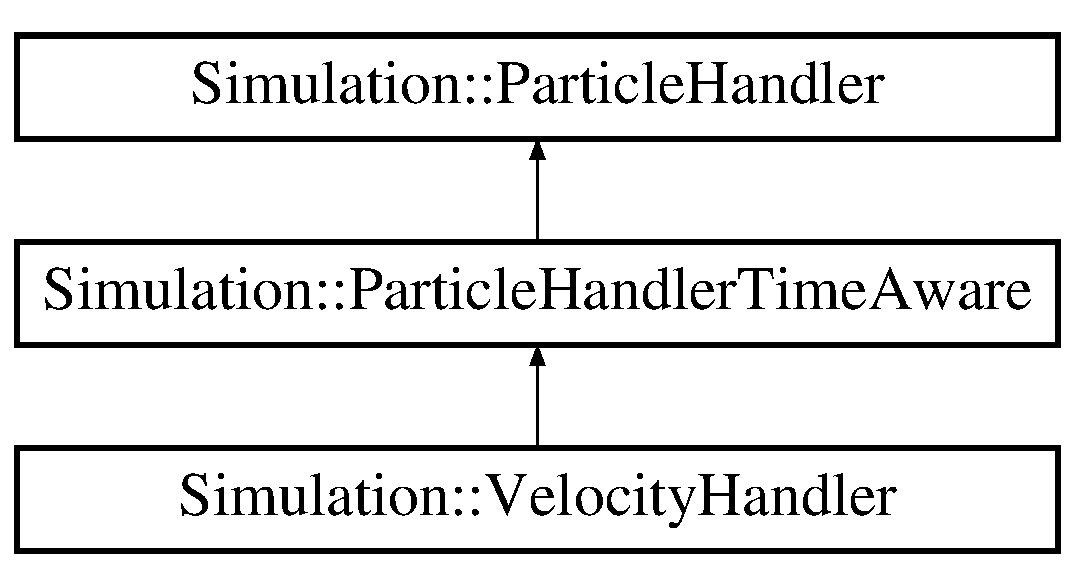
\includegraphics[height=3.000000cm]{classSimulation_1_1VelocityHandler}
\end{center}
\end{figure}
\subsection*{Public Member Functions}
\begin{DoxyCompactItemize}
\item 
\hyperlink{classSimulation_1_1VelocityHandler_abc1da55bdd583040c3fefa6af2b94357}{Velocity\-Handler} (double dt)
\item 
void \hyperlink{classSimulation_1_1VelocityHandler_a5ddac3276478a84466bc7bf3e495b6bb}{compute} (\hyperlink{classSimulation_1_1Particle}{Particle} \&p)
\end{DoxyCompactItemize}
\subsection*{Additional Inherited Members}


\subsection{Constructor \& Destructor Documentation}
\hypertarget{classSimulation_1_1VelocityHandler_abc1da55bdd583040c3fefa6af2b94357}{\index{Simulation\-::\-Velocity\-Handler@{Simulation\-::\-Velocity\-Handler}!Velocity\-Handler@{Velocity\-Handler}}
\index{Velocity\-Handler@{Velocity\-Handler}!Simulation::VelocityHandler@{Simulation\-::\-Velocity\-Handler}}
\subsubsection[{Velocity\-Handler}]{\setlength{\rightskip}{0pt plus 5cm}Simulation\-::\-Velocity\-Handler\-::\-Velocity\-Handler (
\begin{DoxyParamCaption}
\item[{double}]{dt}
\end{DoxyParamCaption}
)\hspace{0.3cm}{\ttfamily [inline]}}}\label{classSimulation_1_1VelocityHandler_abc1da55bdd583040c3fefa6af2b94357}


\subsection{Member Function Documentation}
\hypertarget{classSimulation_1_1VelocityHandler_a5ddac3276478a84466bc7bf3e495b6bb}{\index{Simulation\-::\-Velocity\-Handler@{Simulation\-::\-Velocity\-Handler}!compute@{compute}}
\index{compute@{compute}!Simulation::VelocityHandler@{Simulation\-::\-Velocity\-Handler}}
\subsubsection[{compute}]{\setlength{\rightskip}{0pt plus 5cm}void Simulation\-::\-Velocity\-Handler\-::compute (
\begin{DoxyParamCaption}
\item[{{\bf Particle} \&}]{p}
\end{DoxyParamCaption}
)\hspace{0.3cm}{\ttfamily [inline]}, {\ttfamily [virtual]}}}\label{classSimulation_1_1VelocityHandler_a5ddac3276478a84466bc7bf3e495b6bb}


Reimplemented from \hyperlink{classSimulation_1_1ParticleHandler_a6b1fc310603bc10093d50c674097fd25}{Simulation\-::\-Particle\-Handler}.



The documentation for this class was generated from the following file\-:\begin{DoxyCompactItemize}
\item 
src/\hyperlink{ParticleHandler_8h}{Particle\-Handler.\-h}\end{DoxyCompactItemize}

\chapter{File Documentation}
\hypertarget{FileReader_8cpp}{\section{src/\-File\-Reader.cpp File Reference}
\label{FileReader_8cpp}\index{src/\-File\-Reader.\-cpp@{src/\-File\-Reader.\-cpp}}
}
{\ttfamily \#include \char`\"{}File\-Reader.\-h\char`\"{}}\\*
{\ttfamily \#include \char`\"{}Particle\-Generator.\-h\char`\"{}}\\*
{\ttfamily \#include $<$log4cxx/logger.\-h$>$}\\*
{\ttfamily \#include $<$log4cxx/xml/domconfigurator.\-h$>$}\\*
{\ttfamily \#include $<$fstream$>$}\\*
{\ttfamily \#include $<$sstream$>$}\\*
{\ttfamily \#include $<$iostream$>$}\\*
{\ttfamily \#include $<$cstdlib$>$}\\*
\subsection*{Functions}
\begin{DoxyCompactItemize}
\item 
Logger\-Ptr \hyperlink{FileReader_8cpp_ad9f077322e0adb50e9916be81b49ce73}{file\-Reader\-Logger} (Logger\-::get\-Logger(\char`\"{}File\-Reader\char`\"{}))
\end{DoxyCompactItemize}


\subsection{Function Documentation}
\hypertarget{FileReader_8cpp_ad9f077322e0adb50e9916be81b49ce73}{\index{File\-Reader.\-cpp@{File\-Reader.\-cpp}!file\-Reader\-Logger@{file\-Reader\-Logger}}
\index{file\-Reader\-Logger@{file\-Reader\-Logger}!FileReader.cpp@{File\-Reader.\-cpp}}
\subsubsection[{file\-Reader\-Logger}]{\setlength{\rightskip}{0pt plus 5cm}Logger\-Ptr file\-Reader\-Logger (
\begin{DoxyParamCaption}
\item[{Logger\-::}]{get\-Logger\char`\"{}\-File\-Reader\char`\"{}}
\end{DoxyParamCaption}
)}}\label{FileReader_8cpp_ad9f077322e0adb50e9916be81b49ce73}

\hypertarget{FileReader_8h}{\section{src/\-File\-Reader.h File Reference}
\label{FileReader_8h}\index{src/\-File\-Reader.\-h@{src/\-File\-Reader.\-h}}
}
{\ttfamily \#include \char`\"{}Particle.\-h\char`\"{}}\\*
{\ttfamily \#include $<$vector$>$}\\*
\subsection*{Classes}
\begin{DoxyCompactItemize}
\item 
class \hyperlink{classFileReader}{File\-Reader}
\end{DoxyCompactItemize}

\hypertarget{MaxwellBoltzmannDistribution_8cpp}{\section{src/\-Maxwell\-Boltzmann\-Distribution.cpp File Reference}
\label{MaxwellBoltzmannDistribution_8cpp}\index{src/\-Maxwell\-Boltzmann\-Distribution.\-cpp@{src/\-Maxwell\-Boltzmann\-Distribution.\-cpp}}
}
{\ttfamily \#include \char`\"{}Maxwell\-Boltzmann\-Distribution.\-h\char`\"{}}\\*
{\ttfamily \#include $<$cstdlib$>$}\\*
\subsection*{Functions}
\begin{DoxyCompactItemize}
\item 
static double \hyperlink{MaxwellBoltzmannDistribution_8cpp_a190ff362d45c730aede85bea9359ae2e}{Gauss\-Deviate} ()
\item 
void \hyperlink{MaxwellBoltzmannDistribution_8cpp_aa7ddddfd3f1cbe1443f6dc4ef535f493}{Maxwell\-Boltzmann\-Distribution} (\hyperlink{classSimulation_1_1Particle}{Particle} \&p, double mean\-Velocity, int dimensions)
\end{DoxyCompactItemize}


\subsection{Function Documentation}
\hypertarget{MaxwellBoltzmannDistribution_8cpp_a190ff362d45c730aede85bea9359ae2e}{\index{Maxwell\-Boltzmann\-Distribution.\-cpp@{Maxwell\-Boltzmann\-Distribution.\-cpp}!Gauss\-Deviate@{Gauss\-Deviate}}
\index{Gauss\-Deviate@{Gauss\-Deviate}!MaxwellBoltzmannDistribution.cpp@{Maxwell\-Boltzmann\-Distribution.\-cpp}}
\subsubsection[{Gauss\-Deviate}]{\setlength{\rightskip}{0pt plus 5cm}static double Gauss\-Deviate (
\begin{DoxyParamCaption}
{}
\end{DoxyParamCaption}
)\hspace{0.3cm}{\ttfamily [static]}}}\label{MaxwellBoltzmannDistribution_8cpp_a190ff362d45c730aede85bea9359ae2e}
helper function for \hyperlink{MaxwellBoltzmannDistribution_8cpp_aa7ddddfd3f1cbe1443f6dc4ef535f493}{Maxwell\-Boltzmann\-Distribution()}. Generates a gauss deviate, i.\-e. values according to the normal distribution. \hypertarget{MaxwellBoltzmannDistribution_8cpp_aa7ddddfd3f1cbe1443f6dc4ef535f493}{\index{Maxwell\-Boltzmann\-Distribution.\-cpp@{Maxwell\-Boltzmann\-Distribution.\-cpp}!Maxwell\-Boltzmann\-Distribution@{Maxwell\-Boltzmann\-Distribution}}
\index{Maxwell\-Boltzmann\-Distribution@{Maxwell\-Boltzmann\-Distribution}!MaxwellBoltzmannDistribution.cpp@{Maxwell\-Boltzmann\-Distribution.\-cpp}}
\subsubsection[{Maxwell\-Boltzmann\-Distribution}]{\setlength{\rightskip}{0pt plus 5cm}void Maxwell\-Boltzmann\-Distribution (
\begin{DoxyParamCaption}
\item[{{\bf Simulation\-::\-Particle} \&}]{p, }
\item[{double}]{mean\-Velocity, }
\item[{int}]{dimensions}
\end{DoxyParamCaption}
)}}\label{MaxwellBoltzmannDistribution_8cpp_aa7ddddfd3f1cbe1443f6dc4ef535f493}
add a random velocity according to the Maxwell-\/\-Boltzmann distribution to the particles, with a given mean velocity.

{\ttfamily the} particle to initialize  the mean velocity of the brownian motion for the particle  the number of dimensions to initialize (2 or 3) 
\hypertarget{MaxwellBoltzmannDistribution_8h}{\section{src/\-Maxwell\-Boltzmann\-Distribution.h File Reference}
\label{MaxwellBoltzmannDistribution_8h}\index{src/\-Maxwell\-Boltzmann\-Distribution.\-h@{src/\-Maxwell\-Boltzmann\-Distribution.\-h}}
}
{\ttfamily \#include \char`\"{}Particle.\-h\char`\"{}}\\*
\subsection*{Functions}
\begin{DoxyCompactItemize}
\item 
void \hyperlink{MaxwellBoltzmannDistribution_8h_a1cb55f4f492c94ca061d112968e84d01}{Maxwell\-Boltzmann\-Distribution} (\hyperlink{classSimulation_1_1Particle}{Simulation\-::\-Particle} \&p, double mean\-Velocity, int dimensions)
\end{DoxyCompactItemize}


\subsection{Function Documentation}
\hypertarget{MaxwellBoltzmannDistribution_8h_a1cb55f4f492c94ca061d112968e84d01}{\index{Maxwell\-Boltzmann\-Distribution.\-h@{Maxwell\-Boltzmann\-Distribution.\-h}!Maxwell\-Boltzmann\-Distribution@{Maxwell\-Boltzmann\-Distribution}}
\index{Maxwell\-Boltzmann\-Distribution@{Maxwell\-Boltzmann\-Distribution}!MaxwellBoltzmannDistribution.h@{Maxwell\-Boltzmann\-Distribution.\-h}}
\subsubsection[{Maxwell\-Boltzmann\-Distribution}]{\setlength{\rightskip}{0pt plus 5cm}void Maxwell\-Boltzmann\-Distribution (
\begin{DoxyParamCaption}
\item[{{\bf Simulation\-::\-Particle} \&}]{p, }
\item[{double}]{mean\-Velocity, }
\item[{int}]{dimensions}
\end{DoxyParamCaption}
)}}\label{MaxwellBoltzmannDistribution_8h_a1cb55f4f492c94ca061d112968e84d01}
add a random velocity according to the Maxwell-\/\-Boltzmann distribution to the particles, with a given mean velocity.

{\ttfamily the} particle to initialize  the mean velocity of the brownian motion for the particle  the number of dimensions to initialize (2 or 3) 
\hypertarget{MolSim_8cpp}{\section{src/\-Mol\-Sim.cpp File Reference}
\label{MolSim_8cpp}\index{src/\-Mol\-Sim.\-cpp@{src/\-Mol\-Sim.\-cpp}}
}
{\ttfamily \#include $<$cppunit/ui/text/\-Test\-Runner.\-h$>$}\\*
{\ttfamily \#include \char`\"{}Unit\-Tests.\-h\char`\"{}}\\*
{\ttfamily \#include \char`\"{}output\-Writer/\-X\-Y\-Z\-Writer.\-h\char`\"{}}\\*
{\ttfamily \#include \char`\"{}output\-Writer/\-V\-T\-K\-Writer.\-h\char`\"{}}\\*
{\ttfamily \#include \char`\"{}Particle\-Container.\-h\char`\"{}}\\*
{\ttfamily \#include \char`\"{}Particle\-Handler.\-h\char`\"{}}\\*
{\ttfamily \#include $<$cstring$>$}\\*
{\ttfamily \#include $<$cstdlib$>$}\\*
{\ttfamily \#include $<$iostream$>$}\\*
{\ttfamily \#include $<$ctime$>$}\\*
{\ttfamily \#include $<$log4cxx/logger.\-h$>$}\\*
{\ttfamily \#include $<$log4cxx/xml/domconfigurator.\-h$>$}\\*
\subsection*{Functions}
\begin{DoxyCompactItemize}
\item 
Logger\-Ptr \hyperlink{MolSim_8cpp_a98a9be9d9593b38bab661922890e115f}{logger} (Logger\-::get\-Logger(\char`\"{}main\char`\"{}))
\item 
void \hyperlink{MolSim_8cpp_af4d25832793b65abf538fab0474a8e51}{plot\-Particles} (int iteration)
\item 
int \hyperlink{MolSim_8cpp_a329c95e85f063f49b0daaed5c5b56335}{main} (int argc, char $\ast$argsv\mbox{[}$\,$\mbox{]})
\end{DoxyCompactItemize}
\subsection*{Variables}
\begin{DoxyCompactItemize}
\item 
\hyperlink{classSimulation_1_1ParticleContainer}{Particle\-Container} \hyperlink{MolSim_8cpp_ab06a8478b206d59f33b5b4a630c3804e}{container}
\item 
double \hyperlink{MolSim_8cpp_a00b0c9b1c3ea8bb73a7fc8b53a3961fd}{start\-\_\-time} = 0
\item 
double \hyperlink{MolSim_8cpp_a8c7ea5e69ce954c1d81db1732f9f426a}{end\-\_\-time} = 1000
\item 
double \hyperlink{MolSim_8cpp_a4cfc079302fe9a34fe24637c4e44303a}{delta\-\_\-t} = 0.\-014
\end{DoxyCompactItemize}


\subsection{Function Documentation}
\hypertarget{MolSim_8cpp_a98a9be9d9593b38bab661922890e115f}{\index{Mol\-Sim.\-cpp@{Mol\-Sim.\-cpp}!logger@{logger}}
\index{logger@{logger}!MolSim.cpp@{Mol\-Sim.\-cpp}}
\subsubsection[{logger}]{\setlength{\rightskip}{0pt plus 5cm}Logger\-Ptr logger (
\begin{DoxyParamCaption}
\item[{Logger\-::}]{get\-Logger\char`\"{}main\char`\"{}}
\end{DoxyParamCaption}
)}}\label{MolSim_8cpp_a98a9be9d9593b38bab661922890e115f}
\hypertarget{MolSim_8cpp_a329c95e85f063f49b0daaed5c5b56335}{\index{Mol\-Sim.\-cpp@{Mol\-Sim.\-cpp}!main@{main}}
\index{main@{main}!MolSim.cpp@{Mol\-Sim.\-cpp}}
\subsubsection[{main}]{\setlength{\rightskip}{0pt plus 5cm}int main (
\begin{DoxyParamCaption}
\item[{int}]{argc, }
\item[{char $\ast$}]{argsv\mbox{[}$\,$\mbox{]}}
\end{DoxyParamCaption}
)}}\label{MolSim_8cpp_a329c95e85f063f49b0daaed5c5b56335}
\hypertarget{MolSim_8cpp_af4d25832793b65abf538fab0474a8e51}{\index{Mol\-Sim.\-cpp@{Mol\-Sim.\-cpp}!plot\-Particles@{plot\-Particles}}
\index{plot\-Particles@{plot\-Particles}!MolSim.cpp@{Mol\-Sim.\-cpp}}
\subsubsection[{plot\-Particles}]{\setlength{\rightskip}{0pt plus 5cm}void plot\-Particles (
\begin{DoxyParamCaption}
\item[{int}]{iteration}
\end{DoxyParamCaption}
)}}\label{MolSim_8cpp_af4d25832793b65abf538fab0474a8e51}
plot the particles to a xyz-\/file 

\subsection{Variable Documentation}
\hypertarget{MolSim_8cpp_ab06a8478b206d59f33b5b4a630c3804e}{\index{Mol\-Sim.\-cpp@{Mol\-Sim.\-cpp}!container@{container}}
\index{container@{container}!MolSim.cpp@{Mol\-Sim.\-cpp}}
\subsubsection[{container}]{\setlength{\rightskip}{0pt plus 5cm}{\bf Particle\-Container} container}}\label{MolSim_8cpp_ab06a8478b206d59f33b5b4a630c3804e}
\hypertarget{MolSim_8cpp_a4cfc079302fe9a34fe24637c4e44303a}{\index{Mol\-Sim.\-cpp@{Mol\-Sim.\-cpp}!delta\-\_\-t@{delta\-\_\-t}}
\index{delta\-\_\-t@{delta\-\_\-t}!MolSim.cpp@{Mol\-Sim.\-cpp}}
\subsubsection[{delta\-\_\-t}]{\setlength{\rightskip}{0pt plus 5cm}double delta\-\_\-t = 0.\-014}}\label{MolSim_8cpp_a4cfc079302fe9a34fe24637c4e44303a}
\hypertarget{MolSim_8cpp_a8c7ea5e69ce954c1d81db1732f9f426a}{\index{Mol\-Sim.\-cpp@{Mol\-Sim.\-cpp}!end\-\_\-time@{end\-\_\-time}}
\index{end\-\_\-time@{end\-\_\-time}!MolSim.cpp@{Mol\-Sim.\-cpp}}
\subsubsection[{end\-\_\-time}]{\setlength{\rightskip}{0pt plus 5cm}double end\-\_\-time = 1000}}\label{MolSim_8cpp_a8c7ea5e69ce954c1d81db1732f9f426a}
\hypertarget{MolSim_8cpp_a00b0c9b1c3ea8bb73a7fc8b53a3961fd}{\index{Mol\-Sim.\-cpp@{Mol\-Sim.\-cpp}!start\-\_\-time@{start\-\_\-time}}
\index{start\-\_\-time@{start\-\_\-time}!MolSim.cpp@{Mol\-Sim.\-cpp}}
\subsubsection[{start\-\_\-time}]{\setlength{\rightskip}{0pt plus 5cm}double start\-\_\-time = 0}}\label{MolSim_8cpp_a00b0c9b1c3ea8bb73a7fc8b53a3961fd}

\hypertarget{Particle_8cpp}{\section{src/\-Particle.cpp File Reference}
\label{Particle_8cpp}\index{src/\-Particle.\-cpp@{src/\-Particle.\-cpp}}
}
{\ttfamily \#include \char`\"{}Particle.\-h\char`\"{}}\\*
{\ttfamily \#include $<$log4cxx/logger.\-h$>$}\\*
{\ttfamily \#include $<$log4cxx/xml/domconfigurator.\-h$>$}\\*
{\ttfamily \#include $<$sstream$>$}\\*
{\ttfamily \#include $<$iostream$>$}\\*
\subsection*{Functions}
\begin{DoxyCompactItemize}
\item 
Logger\-Ptr \hyperlink{Particle_8cpp_a3694fa0721c0fdd45c71b26ca2f7fcbc}{particle\-Logger} (Logger\-::get\-Logger(\char`\"{}Particle\char`\"{}))
\item 
std\-::ostream \& \hyperlink{Particle_8cpp_a0a421e41c0d4c59eb91d526f57fcff89}{operator$<$$<$} (std\-::ostream \&stream, \hyperlink{classSimulation_1_1Particle}{Particle} \&p)
\end{DoxyCompactItemize}


\subsection{Function Documentation}
\hypertarget{Particle_8cpp_a0a421e41c0d4c59eb91d526f57fcff89}{\index{Particle.\-cpp@{Particle.\-cpp}!operator$<$$<$@{operator$<$$<$}}
\index{operator$<$$<$@{operator$<$$<$}!Particle.cpp@{Particle.\-cpp}}
\subsubsection[{operator$<$$<$}]{\setlength{\rightskip}{0pt plus 5cm}std\-::ostream\& operator$<$$<$ (
\begin{DoxyParamCaption}
\item[{std\-::ostream \&}]{stream, }
\item[{{\bf Particle} \&}]{p}
\end{DoxyParamCaption}
)}}\label{Particle_8cpp_a0a421e41c0d4c59eb91d526f57fcff89}
\hypertarget{Particle_8cpp_a3694fa0721c0fdd45c71b26ca2f7fcbc}{\index{Particle.\-cpp@{Particle.\-cpp}!particle\-Logger@{particle\-Logger}}
\index{particle\-Logger@{particle\-Logger}!Particle.cpp@{Particle.\-cpp}}
\subsubsection[{particle\-Logger}]{\setlength{\rightskip}{0pt plus 5cm}Logger\-Ptr particle\-Logger (
\begin{DoxyParamCaption}
\item[{Logger\-::}]{get\-Logger\char`\"{}\-Particle\char`\"{}}
\end{DoxyParamCaption}
)}}\label{Particle_8cpp_a3694fa0721c0fdd45c71b26ca2f7fcbc}

\hypertarget{Particle_8h}{\section{src/\-Particle.h File Reference}
\label{Particle_8h}\index{src/\-Particle.\-h@{src/\-Particle.\-h}}
}
{\ttfamily \#include \char`\"{}utils/\-Vector.\-h\char`\"{}}\\*
\subsection*{Classes}
\begin{DoxyCompactItemize}
\item 
class \hyperlink{classSimulation_1_1Particle}{Simulation\-::\-Particle}
\end{DoxyCompactItemize}
\subsection*{Namespaces}
\begin{DoxyCompactItemize}
\item 
\hyperlink{namespaceSimulation}{Simulation}
\end{DoxyCompactItemize}
\subsection*{Functions}
\begin{DoxyCompactItemize}
\item 
std\-::ostream \& \hyperlink{Particle_8h_ab3842a273b79e3e2483a2b066258c187}{operator$<$$<$} (std\-::ostream \&stream, \hyperlink{classSimulation_1_1Particle}{Simulation\-::\-Particle} \&p)
\end{DoxyCompactItemize}


\subsection{Function Documentation}
\hypertarget{Particle_8h_ab3842a273b79e3e2483a2b066258c187}{\index{Particle.\-h@{Particle.\-h}!operator$<$$<$@{operator$<$$<$}}
\index{operator$<$$<$@{operator$<$$<$}!Particle.h@{Particle.\-h}}
\subsubsection[{operator$<$$<$}]{\setlength{\rightskip}{0pt plus 5cm}std\-::ostream\& operator$<$$<$ (
\begin{DoxyParamCaption}
\item[{std\-::ostream \&}]{stream, }
\item[{{\bf Simulation\-::\-Particle} \&}]{p}
\end{DoxyParamCaption}
)}}\label{Particle_8h_ab3842a273b79e3e2483a2b066258c187}

\hypertarget{ParticleContainer_8cpp}{\section{src/\-Particle\-Container.cpp File Reference}
\label{ParticleContainer_8cpp}\index{src/\-Particle\-Container.\-cpp@{src/\-Particle\-Container.\-cpp}}
}
{\ttfamily \#include \char`\"{}Particle\-Container.\-h\char`\"{}}\\*
{\ttfamily \#include \char`\"{}File\-Reader.\-h\char`\"{}}\\*
{\ttfamily \#include $<$log4cxx/logger.\-h$>$}\\*
{\ttfamily \#include $<$log4cxx/xml/domconfigurator.\-h$>$}\\*
\subsection*{Functions}
\begin{DoxyCompactItemize}
\item 
Logger\-Ptr \hyperlink{ParticleContainer_8cpp_af10219948f5d5c140f6a5d4387458cc5}{container\-Logger} (Logger\-::get\-Logger(\char`\"{}Particle\-Contanier\char`\"{}))
\end{DoxyCompactItemize}


\subsection{Function Documentation}
\hypertarget{ParticleContainer_8cpp_af10219948f5d5c140f6a5d4387458cc5}{\index{Particle\-Container.\-cpp@{Particle\-Container.\-cpp}!container\-Logger@{container\-Logger}}
\index{container\-Logger@{container\-Logger}!ParticleContainer.cpp@{Particle\-Container.\-cpp}}
\subsubsection[{container\-Logger}]{\setlength{\rightskip}{0pt plus 5cm}Logger\-Ptr container\-Logger (
\begin{DoxyParamCaption}
\item[{Logger\-::}]{get\-Logger\char`\"{}\-Particle\-Contanier\char`\"{}}
\end{DoxyParamCaption}
)}}\label{ParticleContainer_8cpp_af10219948f5d5c140f6a5d4387458cc5}

\hypertarget{ParticleContainer_8h}{\section{src/\-Particle\-Container.h File Reference}
\label{ParticleContainer_8h}\index{src/\-Particle\-Container.\-h@{src/\-Particle\-Container.\-h}}
}
{\ttfamily \#include $<$vector$>$}\\*
{\ttfamily \#include $<$list$>$}\\*
{\ttfamily \#include \char`\"{}Particle.\-h\char`\"{}}\\*
{\ttfamily \#include \char`\"{}Particle\-Handler.\-h\char`\"{}}\\*
\subsection*{Classes}
\begin{DoxyCompactItemize}
\item 
class \hyperlink{classSimulation_1_1ParticleContainer}{Simulation\-::\-Particle\-Container}
\begin{DoxyCompactList}\small\item\em Container class for managing particles \end{DoxyCompactList}\item 
class \hyperlink{classSimulation_1_1ParticleContainer_1_1ParticleCell}{Simulation\-::\-Particle\-Container\-::\-Particle\-Cell}
\end{DoxyCompactItemize}
\subsection*{Namespaces}
\begin{DoxyCompactItemize}
\item 
\hyperlink{namespaceSimulation}{Simulation}
\end{DoxyCompactItemize}

\hypertarget{ParticleGenerator_8cpp}{\section{src/\-Particle\-Generator.cpp File Reference}
\label{ParticleGenerator_8cpp}\index{src/\-Particle\-Generator.\-cpp@{src/\-Particle\-Generator.\-cpp}}
}
{\ttfamily \#include \char`\"{}Particle\-Generator.\-h\char`\"{}}\\*
{\ttfamily \#include \char`\"{}Maxwell\-Boltzmann\-Distribution.\-h\char`\"{}}\\*

\hypertarget{ParticleGenerator_8h}{\section{src/\-Particle\-Generator.h File Reference}
\label{ParticleGenerator_8h}\index{src/\-Particle\-Generator.\-h@{src/\-Particle\-Generator.\-h}}
}
{\ttfamily \#include $<$vector$>$}\\*
{\ttfamily \#include $<$list$>$}\\*
{\ttfamily \#include \char`\"{}utils/\-Vector.\-h\char`\"{}}\\*
{\ttfamily \#include \char`\"{}Particle.\-h\char`\"{}}\\*
\subsection*{Classes}
\begin{DoxyCompactItemize}
\item 
class \hyperlink{classSimulation_1_1ParticleGenerator}{Simulation\-::\-Particle\-Generator}
\end{DoxyCompactItemize}
\subsection*{Namespaces}
\begin{DoxyCompactItemize}
\item 
\hyperlink{namespaceSimulation}{Simulation}
\end{DoxyCompactItemize}

\hypertarget{ParticleHandler_8h}{\section{src/\-Particle\-Handler.h File Reference}
\label{ParticleHandler_8h}\index{src/\-Particle\-Handler.\-h@{src/\-Particle\-Handler.\-h}}
}
{\ttfamily \#include \char`\"{}Particle.\-h\char`\"{}}\\*
{\ttfamily \#include $<$math.\-h$>$}\\*
{\ttfamily \#include $<$sstream$>$}\\*
{\ttfamily \#include $<$iostream$>$}\\*
\subsection*{Classes}
\begin{DoxyCompactItemize}
\item 
class \hyperlink{classSimulation_1_1ParticleHandler}{Simulation\-::\-Particle\-Handler}
\item 
class \hyperlink{classSimulation_1_1ParticleHandlerTimeAware}{Simulation\-::\-Particle\-Handler\-Time\-Aware}
\item 
class \hyperlink{classSimulation_1_1PositionHandler}{Simulation\-::\-Position\-Handler}
\item 
class \hyperlink{classSimulation_1_1VelocityHandler}{Simulation\-::\-Velocity\-Handler}
\item 
class \hyperlink{classSimulation_1_1GravityHandler}{Simulation\-::\-Gravity\-Handler}
\item 
class \hyperlink{classSimulation_1_1LennardJonesHandler}{Simulation\-::\-Lennard\-Jones\-Handler}
\end{DoxyCompactItemize}
\subsection*{Namespaces}
\begin{DoxyCompactItemize}
\item 
\hyperlink{namespaceSimulation}{Simulation}
\end{DoxyCompactItemize}

\hypertarget{StateWriter_8cpp}{\section{src/\-State\-Writer.cpp File Reference}
\label{StateWriter_8cpp}\index{src/\-State\-Writer.\-cpp@{src/\-State\-Writer.\-cpp}}
}
{\ttfamily \#include \char`\"{}State\-Writer.\-h\char`\"{}}\\*
{\ttfamily \#include $<$iostream$>$}\\*
{\ttfamily \#include $<$fstream$>$}\\*

\hypertarget{StateWriter_8h}{\section{src/\-State\-Writer.h File Reference}
\label{StateWriter_8h}\index{src/\-State\-Writer.\-h@{src/\-State\-Writer.\-h}}
}
{\ttfamily \#include \char`\"{}Particle.\-h\char`\"{}}\\*
{\ttfamily \#include \char`\"{}Particle\-Container.\-h\char`\"{}}\\*
\subsection*{Classes}
\begin{DoxyCompactItemize}
\item 
class \hyperlink{classSimulation_1_1StateWriter}{Simulation\-::\-State\-Writer}
\end{DoxyCompactItemize}
\subsection*{Namespaces}
\begin{DoxyCompactItemize}
\item 
\hyperlink{namespaceSimulation}{Simulation}
\end{DoxyCompactItemize}

\hypertarget{Thermostat_8cpp}{\section{src/\-Thermostat.cpp File Reference}
\label{Thermostat_8cpp}\index{src/\-Thermostat.\-cpp@{src/\-Thermostat.\-cpp}}
}
{\ttfamily \#include \char`\"{}Thermostat.\-h\char`\"{}}\\*
{\ttfamily \#include \char`\"{}Maxwell\-Boltzmann\-Distribution.\-h\char`\"{}}\\*

\hypertarget{Thermostat_8h}{\section{src/\-Thermostat.h File Reference}
\label{Thermostat_8h}\index{src/\-Thermostat.\-h@{src/\-Thermostat.\-h}}
}
{\ttfamily \#include $<$vector$>$}\\*
{\ttfamily \#include $<$list$>$}\\*
{\ttfamily \#include \char`\"{}Particle.\-h\char`\"{}}\\*
{\ttfamily \#include \char`\"{}Particle\-Container.\-h\char`\"{}}\\*
{\ttfamily \#include \char`\"{}Particle\-Handler.\-h\char`\"{}}\\*
\subsection*{Classes}
\begin{DoxyCompactItemize}
\item 
class \hyperlink{classSimulation_1_1Thermostat}{Simulation\-::\-Thermostat}
\begin{DoxyCompactList}\small\item\em Handles temperature of particles in the simulation. \end{DoxyCompactList}\end{DoxyCompactItemize}
\subsection*{Namespaces}
\begin{DoxyCompactItemize}
\item 
\hyperlink{namespaceSimulation}{Simulation}
\end{DoxyCompactItemize}

\hypertarget{UnitTests_8cpp}{\section{src/\-Unit\-Tests.cpp File Reference}
\label{UnitTests_8cpp}\index{src/\-Unit\-Tests.\-cpp@{src/\-Unit\-Tests.\-cpp}}
}
{\ttfamily \#include \char`\"{}Unit\-Tests.\-h\char`\"{}}\\*
{\ttfamily \#include $<$iostream$>$}\\*
{\ttfamily \#include $<$fstream$>$}\\*
{\ttfamily \#include $<$stdio.\-h$>$}\\*
{\ttfamily \#include \char`\"{}Particle\-Handler.\-h\char`\"{}}\\*

\hypertarget{UnitTests_8h}{\section{src/\-Unit\-Tests.h File Reference}
\label{UnitTests_8h}\index{src/\-Unit\-Tests.\-h@{src/\-Unit\-Tests.\-h}}
}
{\ttfamily \#include $<$cppunit/\-Test\-Case.\-h$>$}\\*
{\ttfamily \#include $<$cppunit/\-Test\-Suite.\-h$>$}\\*
{\ttfamily \#include \char`\"{}cppunit/\-Test\-Caller.\-h\char`\"{}}\\*
{\ttfamily \#include \char`\"{}cppunit/\-Test\-Result.\-h\char`\"{}}\\*
{\ttfamily \#include \char`\"{}Particle\-Container.\-h\char`\"{}}\\*
{\ttfamily \#include $<$vector$>$}\\*
\subsection*{Classes}
\begin{DoxyCompactItemize}
\item 
class \hyperlink{classParticleContainerTest}{Particle\-Container\-Test}
\item 
struct \hyperlink{structParticleContainerTest_1_1TestParticle}{Particle\-Container\-Test\-::\-Test\-Particle}
\item 
class \hyperlink{classParticleContainerTest_1_1TestHandler}{Particle\-Container\-Test\-::\-Test\-Handler}
\end{DoxyCompactItemize}

\hypertarget{Vector_8h}{\section{src/utils/\-Vector.h File Reference}
\label{Vector_8h}\index{src/utils/\-Vector.\-h@{src/utils/\-Vector.\-h}}
}
{\ttfamily \#include $<$cmath$>$}\\*
{\ttfamily \#include $<$sstream$>$}\\*
{\ttfamily \#include $<$iostream$>$}\\*
\subsection*{Classes}
\begin{DoxyCompactItemize}
\item 
class \hyperlink{classutils_1_1Vector}{utils\-::\-Vector$<$ type, length $>$}
\item 
class \hyperlink{classutils_1_1Vector}{utils\-::\-Vector$<$ type, length $>$}
\end{DoxyCompactItemize}
\subsection*{Namespaces}
\begin{DoxyCompactItemize}
\item 
\hyperlink{namespaceutils}{utils}
\end{DoxyCompactItemize}
\subsection*{Functions}
\begin{DoxyCompactItemize}
\item 
{\footnotesize template$<$typename type , int length$>$ }\\std\-::ostream \& \hyperlink{Vector_8h_a7e86748c491528fd8005aa230203d7e4}{operator$<$$<$} (std\-::ostream \&stream, const \hyperlink{classutils_1_1Vector}{utils\-::\-Vector}$<$ \hyperlink{classtype}{type}, length $>$ \&v)
\item 
{\footnotesize template$<$typename type , int length$>$ }\\\hyperlink{classutils_1_1Vector}{utils\-::\-Vector}$<$ \hyperlink{classtype}{type}, length $>$ \hyperlink{Vector_8h_afda25e1a1a50d5a1c65f5f1427fc3a99}{operator$\ast$} (double scalar, const \hyperlink{classutils_1_1Vector}{utils\-::\-Vector}$<$ \hyperlink{classtype}{type}, length $>$ \&v)
\end{DoxyCompactItemize}


\subsection{Function Documentation}
\hypertarget{Vector_8h_afda25e1a1a50d5a1c65f5f1427fc3a99}{\index{Vector.\-h@{Vector.\-h}!operator$\ast$@{operator$\ast$}}
\index{operator$\ast$@{operator$\ast$}!Vector.h@{Vector.\-h}}
\subsubsection[{operator$\ast$}]{\setlength{\rightskip}{0pt plus 5cm}template$<$typename type , int length$>$ {\bf utils\-::\-Vector}$<${\bf type}, length$>$ operator$\ast$ (
\begin{DoxyParamCaption}
\item[{double}]{scalar, }
\item[{const {\bf utils\-::\-Vector}$<$ {\bf type}, length $>$ \&}]{v}
\end{DoxyParamCaption}
)}}\label{Vector_8h_afda25e1a1a50d5a1c65f5f1427fc3a99}
\hypertarget{Vector_8h_a7e86748c491528fd8005aa230203d7e4}{\index{Vector.\-h@{Vector.\-h}!operator$<$$<$@{operator$<$$<$}}
\index{operator$<$$<$@{operator$<$$<$}!Vector.h@{Vector.\-h}}
\subsubsection[{operator$<$$<$}]{\setlength{\rightskip}{0pt plus 5cm}template$<$typename type , int length$>$ std\-::ostream\& operator$<$$<$ (
\begin{DoxyParamCaption}
\item[{std\-::ostream \&}]{stream, }
\item[{const {\bf utils\-::\-Vector}$<$ {\bf type}, length $>$ \&}]{v}
\end{DoxyParamCaption}
)}}\label{Vector_8h_a7e86748c491528fd8005aa230203d7e4}
Global operators first 
%--- End generated contents ---

% Index
\newpage
\phantomsection
\addcontentsline{toc}{chapter}{Index}
\printindex

\end{document}
